\documentclass{beamer}
\usepackage{xcolor}
% \usetheme{Marburg}
\usecolortheme{orchid}
\usepackage{pifont}
\usepackage{changepage}
\usepackage{nicefrac}
\usepackage{csquotes}
\usepackage[
backend=biber,
style=alphabetic,
]{biblatex} 
\addbibresource{icgt.bib}
\usepackage{hyperref, xcolor, cmbright,diagbox,colortbl,tikz,graphicx,algorithm2e,cancel,verbatim, graphicx,
listings,float,amsmath,amssymb,array,subfiles,bussproofs,
rotating,MnSymbol,hyperref,mathtools,subcaption,caption}
\newtheorem{proposition}{Proposition}
\usetikzlibrary{overlay-beamer-styles}
\usetikzlibrary{automata, positioning,graphs,shapes, arrows, calc}

\newcommand{\set}[1]{\{#1\}} 
\newcommand{\vertex}[2]{%
  \begin{tikzpicture}[baseline=-1ex]%
    \node [rectangle,rounded corners=2mm,inner sep=0.5mm,fill=#2] {$#1$};%
  \end{tikzpicture}%
}
\newcommand{\graphbox}[8]{
  \begin{scope}[xshift=#2,yshift=#3]
    \draw [rounded corners=2mm] (0,0) rectangle (#4,-#5);
    \node at (0,0mm) [anchor=north west,inner sep=1mm] {#1};
    \begin{scope}[xshift=#4/2+#6,yshift=#7] 
    #8
    \end{scope}
  \end{scope}
}

\newcommand{\opn}[1]{\operatorname{#1}}

\graphicspath{ {.} }

\title{Termination of Injective DPO Graph Rewriting Systems using Subgraph Counting}
\setbeamertemplate{footline}[frame number]
\begin{document}
% \date{\today}
\date{} 

\author{Qi QIU}
\institute[VFU] % (optional)
{
	Supervisor: Xavier URBAIN\\
	Universite Claude Bernard Lyon 1, France \\
    Univ. Grenoble Alpes, France\\
	Projet SAPPORO
} 
  
\maketitle

% \begin{frame}{Plan for myself}
%     \begin{itemize}
%         \item viasualization of graphs and morphisms
%         \item injective DPO graph rewriting
%         \item Termination  
%         \item Example: termination and non-termination
%         \item Introduction of the problem
%         \item Pre-graphs and graphs
%         \item Pre-graph operations
%         \item A simple Running Example for presentation of concepts
%         \item Visualization of Pre-graphs decomposition of DPO diagrams
%         \item Occurrence
%         \item Implicit, explicit and shared occurrences
%         \item Implicitly created and deleted occurrences : example
%         \item X-occurrence in a graph G 
%         \item Termination of a graph rewriting rule $\varphi$ : 1 
%         \item Termination of a graph rewriting rule $\varphi$ : 2
%         \item Analysis of implicit occurrences
%         \item X-non-increasing rule : 1
%         \item X-non-increasing rule : 2
%         \item X-non-increasing rule : 3
%         \item A sufficient termination condition : example
%         \item Conclusion
%     \end{itemize}
% \end{frame}

\begin{frame}{DPO graph rewriting with injective rules}
 \begin{itemize}
    \item Rules $\varphi = (L \overset{l}{\leftarrowtail} K \overset{r}{\rightarrowtail} R)$ consist of two inclusions $l$ and $r$.  
    \item A rule $\varphi' = (L' \overset{l'}{\leftarrowtail} K' \overset{r'}{\rightarrowtail} R')$ is equivalent to $\varphi$ if 
            \begin{center}
                    \resizebox{0.40\textwidth}{!}{
                        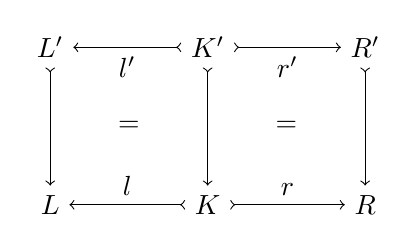
\begin{tikzpicture}
                                \node (I) at (0,0) {$K'$};
                                \node (L) at (-2,0) {$L'$};
                                \node (R) at (2,0) {$R'$};
                                \node (G) at (-2,-2) {$L$};
                                \node (C) at (0,-2) {$K$};
                                \node (H) at (2,-2) {$R$};
                                \draw [>->] (I) to  node [midway,below] {$l'$} (L);
                                \draw [>->] (I) to  node [midway,below] {$r'$} (R);
                                \draw [>->] (L) to node [midway,right] {} (G);
                                \draw [>->] (I) to node [midway,right] { } (C);
                                \draw [>->] (R) to node [midway,left] { } (H);
                                \draw [>->] (C) to node [midway,above] {$l$} (G);
                                \draw [>->] (C) to node [midway,above] {$r$} (H);
                                \node [at=($(I)!.5!(G)$)] {$\mathop{=}$};
                                \node [at=($(I)!.5!(H)$)] {$\mathop{=}$};
                            \end{tikzpicture}
                    }
                \end{center}
    \item 
 Rewriting steps $G \Rightarrow_\varphi H$ are double-pushouts with injective match $m :L' \rightarrowtail G$:
         \begin{center}
          \resizebox{0.40\textwidth}{!}{
              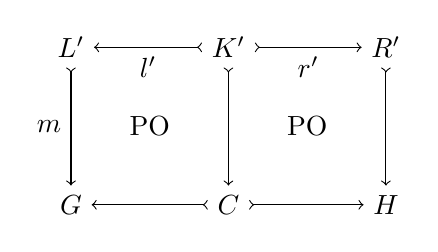
\begin{tikzpicture}
                    \node (I) at (0,0) {$K'$};
                    \node (L) at (-2,0) {$L'$};
                    \node (R) at (2,0) {$R'$};
                    \node (G) at (-2,-2) {$G$};
                    \node (C) at (0,-2) {$C$};
                    \node (H) at (2,-2) {$H$};
                    \draw [>->] (I) to  node [midway,below] {$l'$} (L);
                    \draw [>->] (I) to  node [midway,below] {$r'$} (R);
                    \draw [>->] (L) to node [midway,left] {$m$} (G);
                    \draw [>->] (I) to node [midway,right] { } (C);
                    \draw [>->] (R) to node [midway,left] { } (H);
                    \draw [>->] (C) to node [midway,above] { } (G);
                    \draw [>->] (C) to node [midway,above] { } (H);
                    \node [at=($(I)!.5!(G)$)] {\normalfont PO};
                    \node [at=($(I)!.5!(H)$)] {\normalfont PO};
                  \end{tikzpicture}
          }
      \end{center}
      where all arrows are inclusions and $(L' \overset{l'}{\leftarrowtail} K' \overset{r'}{\rightarrowtail} R')$ is an equivalent rule to $\varphi$.
    %   \item Difference with standard definition: an equivalent rule $\varphi'$ with $\opn{lhs}(\varphi') \subseteq G$ is applied instead of $\varphi$.  
 \end{itemize} 
\end{frame} 


\begin{frame}{Graph}
Finite edge-labeled directed multigraphs
        % \begin{itemize}
        %     \item nodes are represented by circles
        %     \item edges are represented by arrows
        % \end{itemize}
        % \begin{center}
        %     \resizebox{0.25\textwidth}{!}{
        %         \begin{tikzpicture}
        %         \graphbox{}{39mm}{0mm}{35mm}{35mm}{2mm}{-5mm}{
        %                         \coordinate (delta) at (0,-18mm);
        %                         \node[draw,circle] (l1) at ($(delta) + (-1,1.5)$) {};
        %                         \node[draw,circle] (l2) at ($(delta) + (1,1.5)$) {};
        %                         \node[draw,circle] (l3) at ($(delta) + (0,0)$) {};
        %                         \draw[->] (l1) -- (l3) node[midway,left] {s};
        %                         \draw[->] (l2) -- (l3) node[midway,right] {s};
        %                         \draw[->] (l3) edge [loop below] node {0} (l3);
        %                     }
        %         \end{tikzpicture}
        %     }
        % \end{center}

        Visualization of an injective graph morphism $h: L \rightarrowtail R$:
        \begin{itemize}
            \item Codomain $R$ depicted as a supergraph of domain $L$
            \item corresponding elements have the same spatial position
            \item nodes are marked by natural numbers for clarity
            % \item nodes $v$ and $h(v)$ marked by the same natural number
            % \item edges $e$ and $h(e)$ have the same spatial position
        \end{itemize}
        %  \begin{itemize}
        %     \item nodes of domain $L$ are assigned natural numbers 
        %     \item nodes of codomain $R$ are assigned natural numbers of their corresponding nodes in $L$
        %     \item s
        %  \end{itemize}
        \begin{center}
            \resizebox{0.6\textwidth}{!}{
                \begin{tikzpicture}
                    \graphbox{$L$}{39mm}{0mm}{35mm}{35mm}{2mm}{-5mm}{
                        \coordinate (delta) at (0,-18mm);
                        \node[draw,circle] (l1) at ($(delta) + (-1,1.5)$) {1};
                        \node[draw,circle] (l2) at ($(delta) + (1,1.5)$) {2};
                        \node[draw,circle] (l3) at ($(delta) + (0,0)$) {3};
                        \draw[->] (l1) -- (l3) node[midway,left] {s};
                        \draw[->] (l2) -- (l3) node[midway,right] {s};
                        \draw[->] (l3) edge [loop below] node {0} (l3);
                    }
                        \node () at (77mm,-18mm) {$\overset{h}{\rightarrowtail}$};
                    \graphbox{$R$}{80mm}{0mm}{50mm}{35mm}{2mm}{-5mm}{
                        \coordinate (delta) at (-10mm,-18mm);
                        \node[draw,circle] (r1) at ($(delta) + (-1,1.5)$) {1};
                        \node[draw,circle] (r2) at ($(delta) + (0.5,1.5)$) {2};
                        \node[draw,circle] (r3) at ($(delta) + (0,0)$) {3};
                        \node[draw,circle] (r4) at ($(delta) + (1,0)$) {};
                        \draw[->] (r1) edge[bend right] node[midway,left] {s} (r3) ; 
                        \draw[->] (r2) -- (r4) node[midway,right] {s};
                        \draw[->] (r4) edge [loop below] node {0} (r4);
                        \draw[->] (r3) edge [out=190,in=220,looseness=6] node [midway,left] {0} (r3);
                        \node[draw,circle] (r5) at ($(r2) + (1.5,0)$) {};
                        \draw[->] (r5) edge [loop below] node {0} (r5);
                        \draw[->] (r5) edge [loop right] node {0} (r5);
                        \draw[->] (r5) edge [loop left] node {0} (r5);
                        \draw[->] (r1) edge node[midway,left] {s} (r3) ;
                        \draw[->] (r2) edge node[midway,right] {s} (r3) ; 
                        \draw[->] (r3) edge [loop below] node {0} (r3); 
                    }
                    % \graphbox{$R_x$}{40mm}{40mm}{35mm}{35mm}{2mm}{-5mm}{
                    %     \coordinate (delta) at (0,-18mm);
                    %     \coordinate (rxorigin) at ($(interfaceorigin)+(0,6)$);
                    %     \node[draw,circle] (r1) at ($(delta) + (-1,1.5)$) {1};
                    %     \node[draw,circle] (r2) at ($(delta) +  (0.5,1.5)$) {2};
                    %     \node[draw,circle] (r3) at ($(delta) +  (0,0)$) {3};
                    %     \draw[->] (r1) -- (r3) node[midway,left] {s};
                    %     % \draw[->] (r3) edge [loop below] node {0} (r3);
                    % }
                    
                    % \node () at (57mm,2mm) {$\uparrowtail$};
                    % \node () at (38mm,2mm) {$\swarrowtail$};
                    % \node () at (79mm,2mm) {$\searrowtail$};
                \end{tikzpicture}
                }
        \end{center}
    % Inclusion : morphism $h: L \rightarrowtail R$ with $L \subseteq R$.
\end{frame}


\begin{frame}{Termination~\cite{plump2018termination}}
  \begin{itemize}
    \item $\mathcal{R}$ : set of DPO graph rewriting rules
    \item impossibility of transforming any graph $G_0$ indefinitely
      \begin{center}
        $G_0 \Rightarrow_\mathcal{R} G_1 \Rightarrow_\mathcal{R} G_2 \Rightarrow_\mathcal{R} \cdots$
      \end{center}
    \item Guarantees that the non-deterministic strategy
          \begin{center}
              \textcolor{blue}{apply rules as long as possible}
          \end{center}
          returns a result on all inputs
    \item Corresponds to program termination in conventional programming languages:
          \begin{center}
            \textcolor{blue}{program halts on all inputs}
          \end{center}
    \item Undecidable in general
  \end{itemize}
\end{frame}

\begin{frame}{One-rule examples}
    Rule $a$ : 
%   \begin{center}  
\resizebox{0.85\textwidth}{!}{
                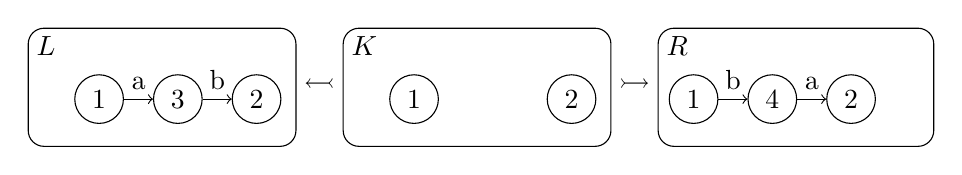
\begin{tikzpicture}[baseline=-3ex]
                    \graphbox{\( L \)}{0mm}{-3mm}{34mm}{15mm}{2mm}{2mm}{
                        \coordinate (o) at (0mm,-11mm); 
                        \node[draw,circle] (l1) at ($(o)+(-10mm,0mm)$) {1};
                        \node[draw,circle] (l2) at ($(l1)+(2,0)$) {2};
                        \node[draw,circle] (l3) at ($(l1) + (1,0)$) {3};
                        \draw[->] (l1) -- (l3) node[midway,above] {a};
                        \draw[->] (l3) -- (l2) node[midway,above] {b};
                    } 
            
                    \graphbox{\( K \)}{40mm}{-3mm}{34mm}{15mm}{2mm}{2mm}{
                        \coordinate (o) at (0mm,-11mm); 
                        \node[draw,circle] (l1) at ($(o)+(-10mm,0mm)$) {1};
                        \node[draw,circle] (l2) at ($(l1)+(2,0)$) {2};
                    }  
            
                    \graphbox{\( R \)}{80mm}{-3mm}{35mm}{15mm}{2mm}{2mm}{
                        \coordinate (o) at (-5mm,-11mm); 
                        \node[draw,circle] (l1) at ($(o)+(-10mm,0mm)$) {1};
                        % \node[draw,circle] (l2) at ($(l1)+(3,0)$) {2};
                        \node[draw,circle] (l3) at ($(l1) + (1,0)$) {4};
                        \node[draw,circle] (l4) at ($(l1) + (2,0)$) {2};
                        \draw[->] (l1) -- (l3) node[midway,above] {b};
                        \draw[->] (l3) -- (l4) node[midway,above] {a};
                        % \draw[->] (l4) -- (l2) node[midway,above] {a};
                    }    
                    \node () at (37mm,-10mm) {\( \leftarrowtail \)}; % K -> L
                    \node () at (77mm,-10mm) {\( \rightarrowtail \)}; % K -> R
                \end{tikzpicture}
                }
            % \end{center}  

\textcolor{blue}{Looping}:
        \begin{center}
          \resizebox{0.85\textwidth}{!}{
            \tikz
            [baseline=-0.5ex]
            { 
                \node (x) at (0,0) {$\bullet$};  
                \node (y) at (1,0) {$\bullet$};
                \node (z) at (0.5,0.86) {$\bullet$};
                \draw[->,red] (x) -- node[midway,below] {a} (y) ;
                \draw[->,red] (y) -- node[midway,right] {b} (z) ;
                \draw[->] (z) -- node[midway,left] {b} (x) ;
            } 
            $\Rightarrow$ 
            \tikz[baseline=-0.5ex]{ 
                \node (x) at (0,0) {$\bullet$};  
                \node (y) at (1,0) {$\bullet$};
                \node (z) at (0.5,0.86) {$\bullet$};
                \draw[->] (x) -- node[midway,below] {b} (y) ;
                \draw[->,red] (y) -- node[midway,right] {a} (z) ;
                \draw[->,red] (z) -- node[midway,left] {b} (x) ;
            }
            $\Rightarrow$ 
            \tikz[baseline=-0.5ex]{ 
                \node (x) at (0,0) {$\bullet$};  
                \node (y) at (1,0) {$\bullet$};
                \node (z) at (0.5,0.86) {$\bullet$};
                \draw[->,red] (x) -- node[midway,below] {b} (y) ;
                \draw[->] (y) -- node[midway,right] {b} (z) ;
                \draw[->,red] (z) -- node[midway,left] {a} (x) ;
            }
            $\Rightarrow$ 
            \tikz[baseline=-0.5ex]{ 
                \node (x) at (0,0) {$\bullet$};   
                \node (y) at (1,0) {$\bullet$};
                \node (z) at (0.5,0.86) {$\bullet$};
                \draw[->,red] (x) -- node[midway,below] {a} (y) ;
                \draw[->,red] (y) -- node[midway,right] {b} (z) ;
                \draw[->] (z) -- node[midway,left] {b} (x) ;
            }
          }
        \end{center}

     Rule $b$:
%   \begin{center}  
                \resizebox{0.85\textwidth}{!}{ 
                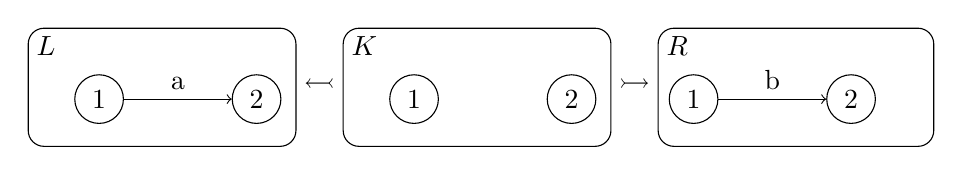
\begin{tikzpicture}[baseline=-3ex]
                    \graphbox{\( L \)}{0mm}{-3mm}{34mm}{15mm}{2mm}{2mm}{
                        \coordinate (o) at (0mm,-11mm); 
                        \node[draw,circle] (l1) at ($(o)+(-10mm,0mm)$) {1};
                        \node[draw,circle] (l2) at ($(l1)+(2,0)$) {2};
                        % \node[draw,circle] (l3) at ($(l1) + (1,0)$) {3};
                        \draw[->] (l1) -- (l2) node[midway,above] {a};
                    } 
            
                    \graphbox{\( K \)}{40mm}{-3mm}{34mm}{15mm}{2mm}{2mm}{
                        \coordinate (o) at (0mm,-11mm); 
                        \node[draw,circle] (l1) at ($(o)+(-10mm,0mm)$) {1};
                        \node[draw,circle] (l2) at ($(l1)+(2,0)$) {2};
                    }  
            
                    \graphbox{\( R \)}{80mm}{-3mm}{35mm}{15mm}{2mm}{2mm}{
                        \coordinate (o) at (-5mm,-11mm); 
                        \node[draw,circle] (l1) at ($(o)+(-10mm,0mm)$) {1};
                        % \node[draw,circle] (l2) at ($(l1)+(3,0)$) {2};
                        % \node[draw,circle] (l3) at ($(l1) + (1,0)$) {4};
                        \node[draw,circle] (l4) at ($(l1) + (2,0)$) {2};
                        \draw[->] (l1) -- (l4) node[midway,above] {b};
                        % \draw[->] (l4) -- (l2) node[midway,above] {a};
                    }    
                    \node () at (37mm,-10mm) {\( \leftarrowtail \)}; % K -> L
                    \node () at (77mm,-10mm) {\( \rightarrowtail \)}; % K -> R
                \end{tikzpicture}
                }
            % \end{center}  

\vspace{2mm}
\textcolor{blue}{Terminating}: the number of edges labeled by \enquote{a} strictly decreases.
        \begin{center}
          \resizebox{0.4\textwidth}{!}{
            \tikz[baseline=-0.5ex]{ 
                \node (x) at (0,0) {$\bullet$};  
                \node (y) at (1,0) {$\bullet$};
                \node (z) at (0.5,0.86) {$\bullet$};
                \draw[->,red] (x) -- node[midway,below] {a} (y) ;
                \draw[->] (y) -- node[midway,right] {b} (z) ;
                \draw[->] (z) -- node[midway,left] {b} (x) ;
            } 
            $\Rightarrow$ 
            \tikz[baseline=-0.5ex]{ 
                \node (x) at (0,0) {$\bullet$};  
                \node (y) at (1,0) {$\bullet$};
                \node (z) at (0.5,0.86) {$\bullet$};
                \draw[->] (x) -- node[midway,below] {b} (y) ;
                \draw[->] (y) -- node[midway,right] {b} (z) ;
                \draw[->] (z) -- node[midway,left] {b} (x) ;
            }
          }
        \end{center}
\end{frame}

\begin{frame}{Termination by Subgraph Counting}
    \begin{itemize}
        \item Rule $\varphi$: 
        % \begin{center} 
        \resizebox{0.9\textwidth}{!}{
            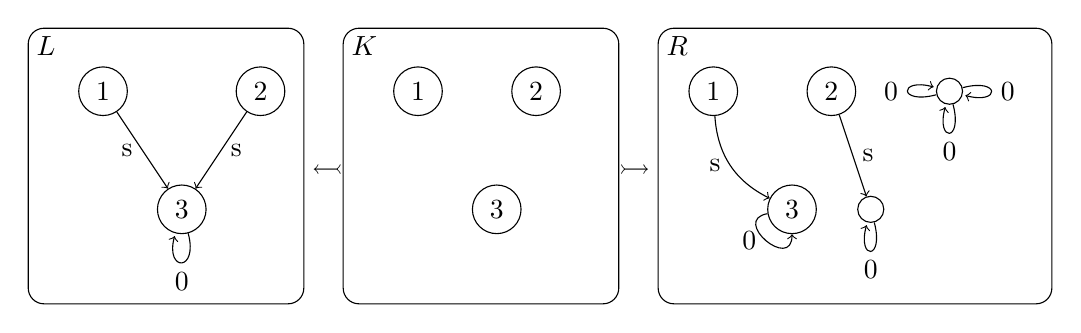
\begin{tikzpicture}
                \graphbox{$L$}{0mm}{0mm}{35mm}{35mm}{2mm}{-5mm}{
                    \coordinate (delta) at (0,-18mm);
                    \node[draw,circle] (l1) at ($(delta) + (-1,1.5)$) {1};
                    \node[draw,circle] (l2) at ($(delta) + (1,1.5)$) {2};
                    \node[draw,circle] (l3) at ($(delta) + (0,0)$) {3};
                    \draw[->] (l1) -- (l3) node[midway,left] {s};
                    \draw[->] (l2) -- (l3) node[midway,right] {s};
                    \draw[->] (l3) edge [loop below] node {0} (l3);
                }
                    \graphbox{$K$}{40mm}{0mm}{35mm}{35mm}{2mm}{-5mm}{
                        \coordinate (delta) at (0,-18mm);
                        \coordinate (interfaceorigin) at ($(delta) +(5,0)$);
                        \node[draw,circle] (r1) at ($(delta) +(-1,1.5)$) {1};
                        \node[draw,circle] (r2) at ($(delta) +(0.5,1.5)$) {2};
                        \node[draw,circle] (r3) at ($(delta) + (0,0)$) {3};
                        % \draw[->] (r1) -- (r3) node[midway,left] {s};
                        % \draw[->] (r3) edge [loop below] node {0} (r3);
                    } 
                    \node () at (38mm,-18mm) {$\leftarrowtail$};
                    \node () at (77mm,-18mm) {$\rightarrowtail$};
                \graphbox{$R$}{80mm}{0mm}{50mm}{35mm}{2mm}{-5mm}{
                    \coordinate (delta) at (-10mm,-18mm);
                    \node[draw,circle] (r1) at ($(delta) + (-1,1.5)$) {1};
                    \node[draw,circle] (r2) at ($(delta) + (0.5,1.5)$) {2};
                    \node[draw,circle] (r3) at ($(delta) + (0,0)$) {3};
                    \node[draw,circle] (r4) at ($(delta) + (1,0)$) {};
                    \draw[->] (r1) edge[bend right] node[midway,left] {s} (r3) ;
                    \draw[->] (r2) -- (r4) node[midway,right] {s};
                    \draw[->] (r4) edge [loop below] node {0} (r4);
                    
                    \draw[->] (r3) edge [out=190,in=270,looseness=3] node[midway,left] {0} (r3);
                    \node[draw,circle] (r5) at ($(r2) + (1.5,0)$) {};
                    \draw[->] (r5) edge [loop below] node {0} (r5);
                    \draw[->] (r5) edge [loop right] node {0} (r5);
                    \draw[->] (r5) edge [loop left] node {0} (r5);
                }
                % \graphbox{$R_x$}{40mm}{40mm}{35mm}{35mm}{2mm}{-5mm}{
                %     \coordinate (delta) at (0,-18mm);
                %     \coordinate (rxorigin) at ($(interfaceorigin)+(0,6)$);
                %     \node[draw,circle] (r1) at ($(delta) + (-1,1.5)$) {1};
                %     \node[draw,circle] (r2) at ($(delta) +  (0.5,1.5)$) {2};
                %     \node[draw,circle] (r3) at ($(delta) +  (0,0)$) {3};
                %     \draw[->] (r1) -- (r3) node[midway,left] {s};
                %     % \draw[->] (r3) edge [loop below] node {0} (r3);
                % }
                
                % \node () at (57mm,2mm) {$\uparrowtail$};
                % \node () at (38mm,2mm) {$\swarrowtail$};
                % \node () at (79mm,2mm) {$\searrowtail$};
            \end{tikzpicture}
            }
    % \end{center}
        \item  Terminating: the number of occurrences of $\tikz[baseline=-0.5ex]{ 
                \node (x) at (0,0) {$\bullet$}; 
                \node (y) at (1,0) {$\bullet$};
                \node (z) at (2,0) {$\bullet$};
                \draw[->] (x) -- (y) node[midway, above] {$s$};
                \draw[->] (z) -- (y) node[midway, above] {$s$};
        }$ strictly decreases
        \item A machine-checkable condition capturing this intuition is desired.
    \end{itemize}
    

   

    
\end{frame}



% \subsection{Pre-graphs and Graphs}
% \begin{frame}{Pre-graphs \( (V, E, \opn{src}, \opn{dst}, l) \)}    
%     \begin{itemize}
%         \item \( \textcolor{red}{V} \subseteq \mathbb{N} \) : finite set of \textcolor{red}{nodes}

%         \item \( \textcolor{red}{E} \subseteq \mathbb{N} \) : finite set of \textcolor{red}{edges}

%         \item \( \textcolor{red}{\opn{src}} : E \to \mathbb{N} \) : \textcolor{red}{source} function

%         \item\( \textcolor{red}{\opn{dst}}: E \to \mathbb{N} \) : \textcolor{red}{target} function

%         \item \textcolor{red}{\( l \)} : edge-\textcolor{red}{labeling} function
%     \end{itemize}

%     Intuition: pre-graphs are graphs which may contain \textcolor{red}{dangling edges}.

%     % A pre-graph with $V=\{1,3\}$:
%     %  \begin{center}
%     %     \resizebox{0.5\textwidth}{!}{
%     %     \begin{tikzpicture}
%     %         \graphbox{\(\)}{00mm}{-20mm}{45mm}{20mm}{2mm}{-5mm}{ 
%     %             \coordinate (o) at (-5mm,-8mm); 
%     %             \node[draw,circle] (l1) at ($(o)+(-10mm,0mm)$) {1};
%     %             % \node[draw,circle] (l2) at ($(l1)+(3,0)$) {};
%     %             \node[draw,circle,dashed,red] (l3) at ($(l1)+(1,0)$) {2};
%     %             \node[draw,circle] (l4) at ($(l1)+(2,0)$) {3};
%     %             \draw[->] (l1) edge[bend right]  node[midway,below] {a} (l3);
%     %             \draw[->] (l1) edge[bend left] node[midway,above] {a}  (l3);
%     %             \draw[->] (l3) -- (l4) node[midway,above] {b};
%     %             % \draw[->] (l4) -- (l2) node[midway,above] {a};
%     %         }  
%     %     \end{tikzpicture} 
%     % }
%     % \end{center}
    
%     % Edge labels are omitted for simplicity.

%     % Edges are distinguished by their spatial positions.
    
% \end{frame}
 
\begin{frame}{Graphs and Pre-graphs}
    Graph are pre-graphs with no dangling edges.

    A graph:
    \begin{center}
        \resizebox{0.5\textwidth}{!}{
        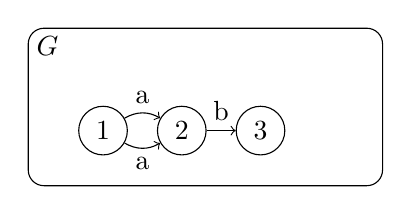
\begin{tikzpicture}
            \graphbox{\( G \)}{00mm}{-20mm}{45mm}{20mm}{2mm}{-5mm}{
                \coordinate (o) at (-5mm,-8mm); 
                \node[draw,circle] (l1) at ($(o)+(-10mm,0mm)$) {1};
                % \node[draw,circle] (l2) at ($(l1)+(3,0)$) {};
                \node[draw,circle] (l3) at ($(l1)+(1,0)$) {2};
                \node[draw,circle] (l4) at ($(l1)+(2,0)$) {3};
                \draw[->] (l1) edge[bend right]  node[midway,below] {a} (l3);
                \draw[->] (l1) edge[bend left] node[midway,above] {a}  (l3);
                \draw[->] (l3) -- (l4) node[midway,above] {b};
                % \draw[->] (l4) -- (l2) node[midway,above] {a};
            }  
        \end{tikzpicture}
    }
    \end{center}

    A pre-graph:

     \begin{center}
        \resizebox{0.5\textwidth}{!}{
        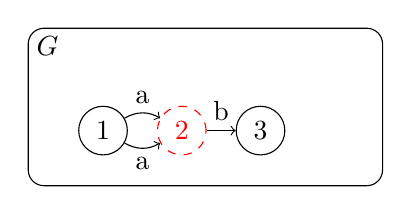
\begin{tikzpicture}
            \graphbox{\( G \)}{00mm}{-20mm}{45mm}{20mm}{2mm}{-5mm}{ 
                \coordinate (o) at (-5mm,-8mm); 
                \node[draw,circle] (l1) at ($(o)+(-10mm,0mm)$) {1};
                % \node[draw,circle] (l2) at ($(l1)+(3,0)$) {};
                \node[draw,circle,dashed,red] (l3) at ($(l1)+(1,0)$) {2};
                \node[draw,circle] (l4) at ($(l1)+(2,0)$) {3};
                \draw[->] (l1) edge[bend right]  node[midway,below] {a} (l3);
                \draw[->] (l1) edge[bend left] node[midway,above] {a}  (l3);
                \draw[->] (l3) -- (l4) node[midway,above] {b};
                % \draw[->] (l4) -- (l2) node[midway,above] {a};
            }  
        \end{tikzpicture} 
    }
    \end{center} 

\end{frame}

\begin{frame}{Pre-graph operations}
    \textcolor{red}{Union} $C \cup R$ of two pre-graphs $C \subseteq G$ and $R \subseteq G$ 
    % \vspace{1mm}
\begin{center}
    \resizebox{\textwidth}{!}{
        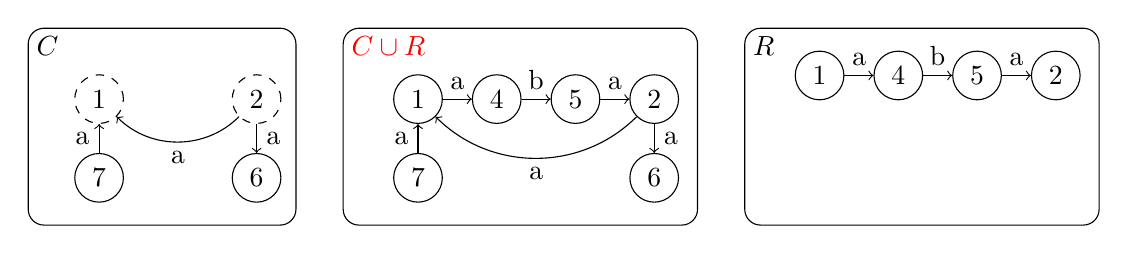
\begin{tikzpicture}  
            \graphbox{\( R \)}{91mm}{-22mm}{45mm}{25mm}{2mm}{2mm}{
                \coordinate (o) at (-5mm,-8mm); 
                \node[draw,circle] (l1) at ($(o)+(-10mm,0mm)$) {1};
                \node[draw,circle] (l2) at ($(l1)+(3,0)$) {2};
                \node[draw,circle] (l3) at ($(l1) + (1,0)$) {4};
                \node[draw,circle] (l4) at ($(l1) + (2,0)$) {5};
                \draw[->] (l1) -- (l3) node[midway,above] {a};
                \draw[->] (l3) -- (l4) node[midway,above] {b};
                \draw[->] (l4) -- (l2) node[midway,above] {a};
            }    
        
            \graphbox{\( C  \)}{0mm}{-22mm}{34mm}{25mm}{2mm}{-3mm}{
                \coordinate (o) at (0mm,-6mm); 
                \node[draw,circle,dashed] (l1) at ($(o)+(-10mm,0mm)$) {1};
                \node[draw,circle,dashed] (l2) at ($(l1)+(2,0)$) {2};
                \node[draw,circle] (l4) at ($(l2) + (0,-1)$) {6};
                \draw[->] (l2) -- (l4) node[midway,right] {a};
                \draw[->] (l2) edge[out=-135,in=-45]node[midway,below] {a} (l1) ;
                \node[ draw,circle] (l6) at ($(l1) + (0,-1)$) {7};
                \draw[<-] (l1) -- (l6) node[midway,left] {a};
            }    

            \graphbox{\textcolor{red}{\(C \cup R \)}}{40mm}{-22mm}{45mm}{25mm}{2mm}{-3mm}{
                \coordinate (o) at (-5mm,-6mm); 
                \node[draw,circle] (l1) at ($(o)+(-10mm,0mm)$) {1};
                \node[draw,circle] (l2) at ($(l1)+(3,0)$) {2};
                \node[draw,circle] (l3) at ($(l1) + (1,0)$) {4};
                \node[draw,circle] (l4) at ($(l1) + (2,0)$) {5};
                \node[ draw,circle] (l5) at ($(l2) + (0,-1)$) {6};
                \node[ draw,circle] (l6) at ($(l1) + (0,-1)$) {7};
                \draw[<-] (l1) -- (l6) node[midway,left] {a};
                \draw[->] (l1) -- (l3) node[midway,above] {a};
                \draw[->] (l3) -- (l4) node[midway,above] {b};
                \draw[->] (l4) -- (l2) node[midway,above] {a};
                \draw[->] (l2) -- (l5) node[midway,right] {a};
                \draw[->] (l2) edge[out=-135,in=-45]node[midway,below] {a} (l1) ;
            }    
             
        \end{tikzpicture}
    }
    \end{center}


    % \textcolor{red}{Intersection} $G \cap H$: 
    % \vspace{1mm}

    % % \begin{center}
    %     \resizebox{0.95\textwidth}{!}{
    %     \begin{tikzpicture}
    %         \graphbox{\( G \)}{0mm}{-22mm}{34mm}{26mm}{2mm}{-3mm}{
    %             \coordinate (o) at (0mm,-6mm); 
    %             \node[draw,circle] (l1) at ($(o)+(-10mm,0mm)$) {1};
    %             \node[draw,circle] (l2) at ($(l1)+(2,0)$) {2};
    %             \node[draw,circle] (l3) at ($(l1) + (1,0)$) {3};
    %             \node[draw,circle] (l4) at ($(l2) + (0,-1)$) {6};
    %             \draw[->] (l1) -- (l3) node[midway,above] {a};
    %             \draw[->] (l3) -- (l2) node[midway,above] {a};
    %             \draw[->] (l2) -- (l4) node[midway,right] {a};
    %             \node[draw,circle] (l6) at ($(l1) + (0,-1)$) {7};
    %             \draw[<-] (l1) -- (l6) node[midway,left] {a};
    %             \draw[->] (l2) edge[out=-135,in=-45]node[midway,below] {a} (l1) ;
    %         }    
    
    %         \graphbox{ \textcolor{red}{\(G \cap H\)}  }{40mm}{-22mm}{34mm}{25mm}{2mm}{-3mm}{
    %             \coordinate (o) at (0mm,-6mm); 
    %             \node[draw,circle] (l1) at ($(o)+(-10mm,0mm)$) {1};
    %             \node[draw,circle] (l2) at ($(l1)+(2,0)$) {2};
    %             \node[draw,circle] (l4) at ($(l2) + (0,-1)$) {6};
    %             \draw[->] (l2) -- (l4) node[midway,right] {a};
    %             \draw[->] (l2) edge[out=-135,in=-45]node[midway,below] {a} (l1) ;
    %             \node[ draw,circle] (l6) at ($(l1) + (0,-1)$) {7};
    %             \draw[<-] (l1) -- (l6) node[midway,left] {a};
    %         }    
    
    %         \graphbox{\( H \)}{80mm}{-22mm}{45mm}{25mm}{2mm}{-6mm}{
    %             \coordinate (o) at (-5mm,-3mm); 
    %             \node[draw,circle] (l1) at ($(o)+(-10mm,0mm)$) {1};
    %             \node[draw,circle] (l2) at ($(l1)+(3,0)$) {2};
    %             \node[draw,circle] (l3) at ($(l1) + (1,0)$) {4};
    %             \node[draw,circle] (l4) at ($(l1) + (2,0)$) {5};
    %             \node[ draw,circle] (l5) at ($(l2) + (0,-1)$) {6};
    %             \node[ draw,circle] (l6) at ($(l1) + (0,-1)$) {7};
    %             \draw[<-] (l1) -- (l6) node[midway,left] {a};
    %             \draw[->] (l1) -- (l3) node[midway,above] {a};
    %             \draw[->] (l3) -- (l4) node[midway,above] {b};
    %             \draw[->] (l4) -- (l2) node[midway,above] {a};
    %             \draw[->] (l2) -- (l5) node[midway,right] {a};
    %             \draw[->] (l2) edge[out=-135,in=-45]node[midway,below] {a} (l1) ;
    %         }    
           
    %         % \node () at (37mm,-33mm) {\( \leftarrowtail \)};
    %         % \node () at (77mm,-33mm) {\( \rightarrowtail \)}; % C -> H
    %     \end{tikzpicture}
    %     }         
    % \end{center}
\textcolor{red}{Relative complement} of $R$ in $H$ where $R \subseteq H$
, denoted $H \setminus R$: 
    % \vspace{1mm} 

    \begin{center}
  \resizebox{\textwidth}{!}{
        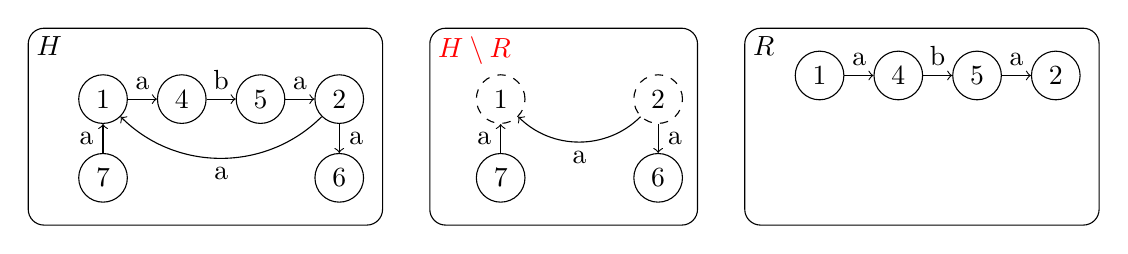
\begin{tikzpicture}  
            \phantom{
                \graphbox{\( G \)}{0mm}{-22mm}{34mm}{22mm}{2mm}{-3mm}{
                }  
            }
            \graphbox{\( R \)}{80mm}{-22mm}{45mm}{25mm}{2mm}{2mm}{
                \coordinate (o) at (-5mm,-8mm); 
                \node[draw,circle] (l1) at ($(o)+(-10mm,0mm)$) {1};
                \node[draw,circle] (l2) at ($(l1)+(3,0)$) {2};
                \node[draw,circle] (l3) at ($(l1) + (1,0)$) {4};
                \node[draw,circle] (l4) at ($(l1) + (2,0)$) {5};
                \draw[->] (l1) -- (l3) node[midway,above] {a};
                \draw[->] (l3) -- (l4) node[midway,above] {b};
                \draw[->] (l4) -- (l2) node[midway,above] {a};
            }    
        
            \graphbox{\textcolor{red}{\( H \setminus R  \)}}{40mm}{-22mm}{34mm}{25mm}{2mm}{-3mm}{
                \coordinate (o) at (0mm,-6mm); 
                \node[draw,dashed,circle] (l1) at ($(o)+(-10mm,0mm)$) {1};
                \node[draw,dashed,circle] (l2) at ($(l1)+(2,0)$) {2};
                \node[draw,circle] (l4) at ($(l2) + (0,-1)$) {6};
                \draw[->] (l2) -- (l4) node[midway,right] {a};
                \draw[->] (l2) edge[out=-135,in=-45]node[midway,below] {a} (l1) ;
                \node[ draw,circle] (l6) at ($(l1) + (0,-1)$) {7};
                \draw[<-] (l1) -- (l6) node[midway,left] {a};
            }    

            \graphbox{\( H \)}{-11mm}{-22mm}{45mm}{25mm}{2mm}{-3mm}{
                \coordinate (o) at (-5mm,-6mm); 
                \node[draw,circle] (l1) at ($(o)+(-10mm,0mm)$) {1};
                \node[draw,circle] (l2) at ($(l1)+(3,0)$) {2};
                \node[draw,circle] (l3) at ($(l1) + (1,0)$) {4};
                \node[draw,circle] (l4) at ($(l1) + (2,0)$) {5};
                \node[ draw,circle] (l5) at ($(l2) + (0,-1)$) {6};
                \node[ draw,circle] (l6) at ($(l1) + (0,-1)$) {7};
                \draw[<-] (l1) -- (l6) node[midway,left] {a};
                \draw[->] (l1) -- (l3) node[midway,above] {a};
                \draw[->] (l3) -- (l4) node[midway,above] {b};
                \draw[->] (l4) -- (l2) node[midway,above] {a};
                \draw[->] (l2) -- (l5) node[midway,right] {a};
                \draw[->] (l2) edge[out=-135,in=-45]node[midway,below] {a} (l1) ;
            }    
            % \node () at (102mm,-18mm) {\( \downarrowtail \)};
            % \node () at (77mm,-33mm) {\( \rightarrowtail \)}; % C -> H
        \end{tikzpicture}
    }
    \end{center}

    % Remark : \textcolor{red}{$H \setminus R$ is not always a graph.}
\end{frame}



% \begin{frame}{Graph morphism $h : G \rightarrow H$}
%    Function preserving graph structure and edge-labels.

%    Domain : $G$ 

%    Codomain :$H$

%     Injective morphism : $\rightarrowtail$

%     % Isomorphisms : bijective morphisms\\

%     \textcolor{red}{Inclusion} if 
%         \begin{itemize}
%             \item $G$ is a subgraph of $H$
%             \item $h$ maps every node and edge to itself
%         \end{itemize}

%     Visualization:
%      \begin{center} 
%             \resizebox{0.8\textwidth}{!}{
%             \begin{tikzpicture}
%                     \graphbox{\( \)}{40mm}{-22mm}{34mm}{25mm}{2mm}{-3mm}{
%                         \coordinate (o) at (0mm,-8mm); 
%                         \node[draw,circle] (l1) at ($(o)+(-10mm,0mm)$) {1};
%                         \node[draw,circle] (l2) at ($(l1)+(2,0)$) {2};
%                         \node[draw,circle] (l4) at ($(l2) + (0,-1)$) {6};
%                         \draw[->] (l2) -- (l4) node[midway,right] {a};
%                         \draw[->] (l2) edge[out=-135,in=-45]node[midway,below] {a} (l1) ;
%                         \node[ draw,circle] (l6) at ($(l1) + (0,-1)$) {7};
%                         \draw[<-] (l1) -- (l6) node[midway,left] {a};
%                     }    
%                     \graphbox{\( \)}{80mm}{-22mm}{45mm}{25mm}{2mm}{-3mm}{
%                         \coordinate (o) at (-5mm,-8mm); 
%                         \node[draw,circle] (l1) at ($(o)+(-10mm,0mm)$) {1};
%                         \node[draw,circle] (l2) at ($(l1)+(3,0)$) {2};
%                         \node[draw,circle] (l3) at ($(l1) + (1,0)$) {4};
%                         \node[draw,circle] (l4) at ($(l1) + (2,0)$) {5};
%                         \node[ draw,circle] (l5) at ($(l2) + (0,-1)$) {6};
%                         \node[ draw,circle] (l6) at ($(l1) + (0,-1)$) {7};
%                         \draw[<-] (l1) -- (l6) node[midway,left] {a};
%                         \draw[->] (l1) -- (l3) node[midway,above] {a};
%                         \draw[->] (l3) -- (l4) node[midway,above] {b};
%                         \draw[->] (l4) -- (l2) node[midway,above] {a};
%                         \draw[->] (l2) -- (l5) node[midway,right] {a};
%                         \draw[->] (l2) edge[out=-135,in=-45]node[midway,below] {a} (l1) ;
%                     }    
%                     \node () at (77mm,-33mm) {\( \rightarrowtail \)}; % C -> H
%             \end{tikzpicture}
%             }  
%     \end{center}

%     % All \alert{graphs} in this presentation are \alert{up to isomorphism}.
%  \end{frame}

% \subsection{Pushout and pushout complement}
% \begin{frame}{Pushout of a pair of inclusions \( L \overset{\alpha}{\leftarrowtail} K \overset{\beta}{\rightarrowtail} C \)}

%     Suppose $L \cap C = K$
%     % \begin{itemize}
%     %     \item $\alpha$, $\beta$ inclusions
%     %     \item $L \cap C = K$
%     % \end{itemize}

%     \textcolor{red}{Pushout} : \( L \overset{\beta'}{\rightarrowtail} L \cup C \overset{\alpha'}{\leftarrowtail} R \) with $\alpha'$, $\beta'$ inclusions\\

%     Example:

%     % Pushout object : $L \cup C$


%     % \( L \overset{\alpha}{\leftarrowtail} K \overset{\beta}{\rightarrowtail} C \): a pair of injective homomorphisms with domain \( K \)


%     % A pushout of a pair of injective homomorphisms \( L \overset{\alpha}{\leftarrowtail} K \overset{\beta}{\rightarrowtail} C \) is a pair of injective homomorphisms \( L \overset{\beta'}{\rightarrowtail} G \overset{\alpha'}{\leftarrowtail} R \) as shown below:
    
%     \begin{center}  
%         \resizebox{0.9\textwidth}{!}{
%         \begin{tikzpicture} 
%             \graphbox{\( L \)}{40mm}{20mm}{34mm}{12mm}{2mm}{2mm}{
%                 \coordinate (o) at (0mm,-8mm); 
%                 \node[draw,circle] (l1) at ($(o)+(-10mm,0mm)$) {1};
%                 \node[draw,circle] (l2) at ($(l1)+(2,0)$) {2};
%                 \node[draw,circle,red] (l3) at ($(l1) + (1,0)$) {3};
%                 \draw[->,red] (l1) -- (l3) node[midway,above] {a};
%                 \draw[->,red] (l3) -- (l2) node[midway,above] {a};
%             } 
    
%             \graphbox{\( K \)}{0mm}{0mm}{34mm}{12mm}{2mm}{2mm}{
%                 \coordinate (o) at (0mm,-8mm); 
%                 \node[draw,circle] (l1) at ($(o)+(-10mm,0mm)$) {1};
%                 \node[draw,circle] (l2) at ($(l1)+(2,0)$) {2};
%             }  
%             \graphbox{\(G = L \cup C \)}{90mm}{5mm}{34mm}{27mm}{2mm}{-3mm}{
%                 \coordinate (o) at (0mm,-8mm); 
%                 \node[draw,circle] (l1) at ($(o)+(-10mm,0mm)$) {1};
%                 \node[draw,circle] (l2) at ($(l1)+(2,0)$) {2};
%                 \node[draw,circle,red] (l3) at ($(l1) + (1,0)$) {3};
%                 \node[draw,circle,blue] (l4) at ($(l2) + (0,-1)$) {6};
%                 \draw[->,red] (l1) -- (l3) node[midway,above] {a};
%                 \draw[->,red] (l3) -- (l2) node[midway,above] {a};
%                 \draw[->,blue] (l2) -- (l4) node[midway,right] {a};
%                 \node[draw,circle,blue] (l6) at ($(l1) + (0,-1)$) {7};
%                 \draw[<-,blue] (l1) -- (l6) node[midway,left] {a};
%                 \draw[->,blue] (l2) edge[out=-135,in=-45]node[midway,below] {a} (l1) ;
%             }   
     
%             \graphbox{\( C \)}{40mm}{-20mm}{34mm}{27mm}{2mm}{-3mm}{
%                 \coordinate (o) at (0mm,-8mm); 
%                 \node[draw,circle] (l1) at ($(o)+(-10mm,0mm)$) {1};
%                 \node[draw,circle] (l2) at ($(l1)+(2,0)$) {2};
%                 \node[draw,circle,blue] (l4) at ($(l2) + (0,-1)$) {6};
%                 \draw[->,blue] (l2) -- (l4) node[midway,right] {a};
%                 \draw[->,blue] (l2) edge[out=-135,in=-45]node[midway,below] {a} (l1) ;
%                 \node[ draw,circle,blue] (l6) at ($(l1) + (0,-1)$) {7};
%                 \draw[<-,blue] (l1) -- (l6) node[midway,left] {a};
%             }      
%             % K to L
%             \draw[>->] (17mm,5mm) -- node[above] {$\alpha$} (37mm,15mm);
%             % C to G
%             \draw[>->] (76mm,-28mm)-- node[below] {$\alpha'$} (104mm,-24mm) ;
%             % K to C
%             \draw[>->] (17mm,-17mm) -- node[below] {$\beta$} (37mm,-28mm);
%             % L to G
%             \draw[>->] (76mm,16mm) -- node[above] {$\beta'$} (104mm,7mm);
%             \node () at (57mm,-6mm) {$PO$};
%         \end{tikzpicture}
%         }
%     \end{center}

%     % \( L \overset{\beta'}{\rightarrowtail} G \overset{\alpha'}{\leftarrowtail} R \): a \textcolor{red}{pushout} of  \( L \overset{\alpha}{\leftarrowtail} K \overset{\beta}{\rightarrowtail} C \)
    
%     % \textcolor{red}{Pushout object} $G$: gluing of \( L \) and \( C \) along \( K \)
% \end{frame}

% \begin{frame}{Pushout complement of a pair of inclusions \( K \overset{\alpha}{\leftarrowtail} L \overset{\beta'}{\rightarrowtail} G \)}
%     % Suppose : $\alpha$, $\beta'$ inclusions

%     \textcolor{red}{Pushout complement} : \( K \overset{\beta}{\rightarrowtail} (G\setminus L)\cup K \overset{\alpha'}{\leftarrowtail} G \) with $\alpha$, $\beta$ inclusions

%     Example: 

%     % Pushout complement object : $(G\setminus L)\cup K$: 

%     \begin{center} 
%         \resizebox{0.9\textwidth}{!}{
%         \begin{tikzpicture} 
%             \graphbox{\( L \)}{40mm}{20mm}{34mm}{12mm}{2mm}{2mm}{
%                 \coordinate (o) at (0mm,-8mm); 
%                 \node[draw,circle] (l1) at ($(o)+(-10mm,0mm)$) {1};
%                 \node[draw,circle] (l2) at ($(l1)+(2,0)$) {2};
%                 \node[draw,circle,red] (l3) at ($(l1) + (1,0)$) {3};
%                 \draw[->,red] (l1) -- (l3) node[midway,above] {a};
%                 \draw[->,red] (l3) -- (l2) node[midway,above] {a};
%             } 
    
%             \graphbox{\( K \)}{0mm}{0mm}{34mm}{12mm}{2mm}{2mm}{
%                 \coordinate (o) at (0mm,-8mm); 
%                 \node[draw,circle] (l1) at ($(o)+(-10mm,0mm)$) {1};
%                 \node[draw,circle] (l2) at ($(l1)+(2,0)$) {2};
%             }  
%             \graphbox{\(G \)}{90mm}{5mm}{34mm}{27mm}{2mm}{-3mm}{
%                 \coordinate (o) at (0mm,-8mm); 
%                 \node[draw,circle] (l1) at ($(o)+(-10mm,0mm)$) {1};
%                 \node[draw,circle] (l2) at ($(l1)+(2,0)$) {2};
%                 \node[draw,circle,red] (l3) at ($(l1) + (1,0)$) {3};
%                 \node[draw,circle,blue] (l4) at ($(l2) + (0,-1)$) {6};
%                 \draw[->,red] (l1) -- (l3) node[midway,above] {a};
%                 \draw[->,red] (l3) -- (l2) node[midway,above] {a};
%                 \draw[->,blue] (l2) -- (l4) node[midway,right] {a};
%                 \node[draw,circle,blue] (l6) at ($(l1) + (0,-1)$) {7};
%                 \draw[<-,blue] (l1) -- (l6) node[midway,left] {a};
%                 \draw[->,blue] (l2) edge[out=-135,in=-45]node[midway,below] {a} (l1) ;
%             }   
     
%             \graphbox{\( C = (G \setminus L) \cup K  \)}{40mm}{-20mm}{34mm}{27mm}{2mm}{-3mm}{
%                 \coordinate (o) at (0mm,-8mm); 
%                 \node[draw,circle] (l1) at ($(o)+(-10mm,0mm)$) {1};
%                 \node[draw,circle] (l2) at ($(l1)+(2,0)$) {2};
%                 \node[draw,circle,blue] (l4) at ($(l2) + (0,-1)$) {6};
%                 \draw[->,blue] (l2) -- (l4) node[midway,right] {a};
%                 \draw[->,blue] (l2) edge[out=-135,in=-45]node[midway,below] {a} (l1) ;
%                 \node[ draw,circle,blue] (l6) at ($(l1) + (0,-1)$) {7};
%                 \draw[<-,blue] (l1) -- (l6) node[midway,left] {a};
%             }      
%             % K to L
%             \draw[>->] (17mm,5mm) -- node[above] {$\alpha$} (37mm,15mm);
%             % C to G
%             \draw[>->] (76mm,-28mm)-- node[below] {$\alpha'$} (104mm,-24mm) ;
%             % K to C
%             \draw[>->] (17mm,-17mm) -- node[below] {$\beta$} (37mm,-28mm);
%             % L to G
%             \draw[>->] (76mm,16mm) -- node[above] {$\beta'$} (104mm,7mm);
%             \node () at (57mm,-6mm) {$PO$};
%         \end{tikzpicture}
%         }
%     \end{center}

%     % $K \overset{\beta}{\rightarrowtail} C \overset{\alpha'}{\rightarrowtail} G$ 
%     % : a \alert{pushout complement} of $K \overset{\alpha}{\rightarrowtail} L \overset{\beta'}{\rightarrowtail} G$

%     % $C$ : \alert{pushout complement object} \\
%     % \begin{theorem}[ref handbook p.188]
%     %     if pushout object exists, then it is unique up to isomorphism.
%     % \end{theorem}
% \end{frame}

\begin{frame}{Running example}
    % Rule : a pair of inclusions $L \leftarrowtail K \rightarrowtail R$ with $L \cap R = K$

    % Motivating example:
    % \begin{center}
    %     \resizebox{\textwidth}{!}{
    %         \begin{tikzpicture}
    %             \graphbox{$L$}{0mm}{0mm}{35mm}{35mm}{2mm}{-5mm}{
    %                 \coordinate (delta) at (0,-18mm);
    %                 \node[draw,circle] (l1) at ($(delta) + (-1,1.5)$) {1};
    %                 \node[draw,circle] (l2) at ($(delta) + (1,1.5)$) {2};
    %                 \node[draw,circle] (l3) at ($(delta) + (0,0)$) {3};
    %                 \draw[->] (l1) -- (l3) node[midway,left] {s};
    %                 \draw[->] (l2) -- (l3) node[midway,right] {s};
    %                 \draw[->] (l3) edge [loop below] node {0} (l3);
    %             }
    %                 \graphbox{$K$}{40mm}{0mm}{35mm}{35mm}{2mm}{-5mm}{
    %                     \coordinate (delta) at (0,-18mm);
    %                     \coordinate (interfaceorigin) at ($(delta) +(5,0)$);
    %                     \node[draw,circle] (r1) at ($(delta) +(-1,1.5)$) {1};
    %                     \node[draw,circle] (r2) at ($(delta) +(0.5,1.5)$) {2};
    %                     \node[draw,circle] (r3) at ($(delta) + (0,0)$) {3};
    %                     % \draw[->] (r1) -- (r3) node[midway,left] {s};
    %                     % \draw[->] (r3) edge [loop below] node {0} (r3);
    %                 } 
    %                 \node () at (38mm,-18mm) {$\leftarrowtail$};
    %                 \node () at (77mm,-18mm) {$\rightarrowtail$};
    %             \graphbox{$R$}{80mm}{0mm}{50mm}{35mm}{2mm}{-5mm}{
    %                 \coordinate (delta) at (-10mm,-18mm);
    %                 \node[draw,circle] (r1) at ($(delta) + (-1,1.5)$) {1};
    %                 \node[draw,circle] (r2) at ($(delta) + (0.5,1.5)$) {2};
    %                 \node[draw,circle] (r3) at ($(delta) + (0,0)$) {3};
    %                 \node[draw,circle] (r4) at ($(delta) + (1,0)$) {};
    %                 \draw[->] (r1) edge[bend right] node[midway,left] {s} (r3) ;
    %                 \draw[->] (r2) -- (r4) node[midway,right] {s};
    %                 \draw[->] (r4) edge [loop below] node {0} (r4);
                    
    %                 \draw[->] (r3) edge [out=190,in=270,looseness=3] node[midway,left] {0} (r3);
    %                 \node[draw,circle] (r5) at ($(r2) + (1.5,0)$) {};
    %                 \draw[->] (r5) edge [loop below] node {0} (r5);
    %                 \draw[->] (r5) edge [loop right] node {0} (r5);
    %                 \draw[->] (r5) edge [loop left] node {0} (r5);
    %             }
    %             % \graphbox{$R_x$}{40mm}{40mm}{35mm}{35mm}{2mm}{-5mm}{
    %             %     \coordinate (delta) at (0,-18mm);
    %             %     \coordinate (rxorigin) at ($(interfaceorigin)+(0,6)$);
    %             %     \node[draw,circle] (r1) at ($(delta) + (-1,1.5)$) {1};
    %             %     \node[draw,circle] (r2) at ($(delta) +  (0.5,1.5)$) {2};
    %             %     \node[draw,circle] (r3) at ($(delta) +  (0,0)$) {3};
    %             %     \draw[->] (r1) -- (r3) node[midway,left] {s};
    %             %     % \draw[->] (r3) edge [loop below] node {0} (r3);
    %             % }
                
    %             % \node () at (57mm,2mm) {$\uparrowtail$};
    %             % \node () at (38mm,2mm) {$\swarrowtail$};
    %             % \node () at (79mm,2mm) {$\searrowtail$};
    %         \end{tikzpicture}
    %         }
    % \end{center}

         \begin{center} 
            \resizebox{\textwidth}{!}{
            \begin{tikzpicture}
                \graphbox{\( L \)}{0mm}{-3mm}{34mm}{12mm}{2mm}{2mm}{
                    \coordinate (o) at (0mm,-8mm); 
                    \node[draw,circle] (l1) at ($(o)+(-10mm,0mm)$) {1};
                    \node[draw,circle] (l2) at ($(l1)+(2,0)$) {2};
                    \node[draw,circle] (l3) at ($(l1) + (1,0)$) {};
                    \draw[->] (l1) -- (l3) node[midway,above] {a};
                    \draw[->] (l3) -- (l2) node[midway,above] {a};
                } 
        
                \graphbox{\( K \)}{40mm}{-3mm}{34mm}{12mm}{2mm}{2mm}{
                    \coordinate (o) at (0mm,-8mm); 
                    \node[draw,circle] (l1) at ($(o)+(-10mm,0mm)$) {1};
                    \node[draw,circle] (l2) at ($(l1)+(2,0)$) {2};
                }  
        
                \graphbox{\( R \)}{80mm}{-3mm}{45mm}{12mm}{2mm}{2mm}{
                    \coordinate (o) at (-5mm,-8mm); 
                    \node[draw,circle] (l1) at ($(o)+(-10mm,0mm)$) {1};
                    \node[draw,circle] (l2) at ($(l1)+(3,0)$) {2};
                    \node[draw,circle] (l3) at ($(l1) + (1,0)$) {};
                    \node[draw,circle] (l4) at ($(l1) + (2,0)$) {};
                    \draw[->] (l1) -- (l3) node[midway,above] {a};
                    \draw[->] (l3) -- (l4) node[midway,above] {b};
                    \draw[->] (l4) -- (l2) node[midway,above] {a};
                }    
                \node () at (37mm,-8mm) {\( \overset{l}{\leftarrowtail} \)}; % K -> L
                \node () at (77mm,-8mm) {\( \overset{r}{\rightarrowtail} \)}; % K -> R
            \end{tikzpicture}
            }         
        \end{center}

    It replaces chain  \tikz[baseline=-0.5ex]{ 
        \node (x) at (0,0) {$\bullet$};  
        \node (y) at (1,0) {$\bullet$};
        \node (z) at (2,0) {$\bullet$};
        \draw[->] (x) -- node[midway,above] {a} (y) ;
        \draw[->] (y) -- node[midway,above] {a} (z) ;
        } with \tikz[baseline=-0.5ex]{ 
        \node (x) at (0,0) {$\bullet$};  
        \node (y) at (1,0) {$\bullet$};
        \node (z) at (2,0) {$\bullet$};
        \node (w) at (3,0) {$\bullet$};
        \draw[->] (x) -- node[midway,above] {a} (y) ;
        \draw[->] (y) -- node[midway,above] {b} (z) ;
        \draw[->] (z) -- node[midway,above] {a} (w) ;
        }.
\end{frame}

% \begin{frame}{Equivalent rules}
%     $\alpha = L \overset{l}{\leftarrowtail} K \overset{r}{\rightarrowtail} R$ : rule

%     $\beta =  L' \overset{l'}{\leftarrowtail} K' \overset{r'}{\rightarrowtail} R'$ : rule
    
%     \textcolor{red}{Equivalent} if 
%     \begin{itemize}
%         \item there \textcolor{red}{exist isomorphisms $f,g,h$}
%         \item $l \circ g = f \circ l'$
%         \item $r \circ g = h \circ r'$
%     \end{itemize}

%     Example:

%    \begin{center} 
%             \resizebox{\textwidth}{!}{
%             \begin{tikzpicture}
%                 \graphbox{\( L \)}{0mm}{-3mm}{34mm}{12mm}{2mm}{2mm}{
%                     \coordinate (o) at (0mm,-8mm); 
%                     \node[draw,circle] (l1) at ($(o)+(-10mm,0mm)$) {6};
%                     \node[draw,circle] (l2) at ($(l1)+(2,0)$) {7};
%                     \node[draw,circle] (l3) at ($(l1) + (1,0)$) {8};
%                     \draw[->] (l1) -- (l3) node[midway,above] {a};
%                     \draw[->] (l3) -- (l2) node[midway,above] {a};
%                 } 
        
%                 \graphbox{\( K \)}{40mm}{-3mm}{34mm}{12mm}{2mm}{2mm}{
%                     \coordinate (o) at (0mm,-8mm); 
%                     \node[draw,circle] (l1) at ($(o)+(-10mm,0mm)$) {6};
%                     \node[draw,circle] (l2) at ($(l1)+(2,0)$) {7};
%                 }  
        
%                 \graphbox{\( R \)}{80mm}{-3mm}{45mm}{12mm}{2mm}{2mm}{
%                     \coordinate (o) at (-5mm,-8mm); 
%                     \node[draw,circle] (l1) at ($(o)+(-10mm,0mm)$) {6};
%                     \node[draw,circle] (l2) at ($(l1)+(3,0)$) {7};
%                     \node[draw,circle] (l3) at ($(l1) + (1,0)$) {9};
%                     \node[draw,circle] (l4) at ($(l1) + (2,0)$) {10};
%                     \draw[->] (l1) -- (l3) node[midway,above] {a};
%                     \draw[->] (l3) -- (l4) node[midway,above] {b};
%                     \draw[->] (l4) -- (l2) node[midway,above] {a};
%                 }    
%                 \node () at (37mm,-8mm) {\( \overset{\textcolor{red}{l}}{\leftarrowtail} \)}; % K -> L
%                 \node () at (77mm,-8mm) {\( \overset{\textcolor{red}{r}}{\rightarrowtail} \)}; % K -> R
%                 \graphbox{\( L' \)}{0mm}{-33mm}{34mm}{12mm}{2mm}{2mm}{
%                     \coordinate (o) at (0mm,-8mm); 
%                     \node[draw,circle] (l1) at ($(o)+(-10mm,0mm)$) {1};
%                     \node[draw,circle] (l2) at ($(l1)+(2,0)$) {2};
%                     \node[draw,circle] (l3) at ($(l1) + (1,0)$) {3};
%                     \draw[->] (l1) -- (l3) node[midway,above] {a};
%                     \draw[->] (l3) -- (l2) node[midway,above] {a};
%                 } 
        
%                 \graphbox{\( K' \)}{40mm}{-33mm}{34mm}{12mm}{2mm}{2mm}{
%                     \coordinate (o) at (0mm,-8mm); 
%                     \node[draw,circle] (l1) at ($(o)+(-10mm,0mm)$) {1};
%                     \node[draw,circle] (l2) at ($(l1)+(2,0)$) {2};
%                 }  
        
%                 \graphbox{\( R' \)}{80mm}{-33mm}{45mm}{12mm}{2mm}{2mm}{
%                     \coordinate (o) at (-5mm,-8mm); 
%                     \node[draw,circle] (l1) at ($(o)+(-10mm,0mm)$) {1};
%                     \node[draw,circle] (l2) at ($(l1)+(3,0)$) {2};
%                     \node[draw,circle] (l3) at ($(l1) + (1,0)$) {4};
%                     \node[draw,circle] (l4) at ($(l1) + (2,0)$) {5};
%                     \draw[->] (l1) -- (l3) node[midway,above] {a};
%                     \draw[->] (l3) -- (l4) node[midway,above] {b};
%                     \draw[->] (l4) -- (l2) node[midway,above] {a};
%                 }    
%                 \node () at (37mm,-38mm) {\( \overset{\textcolor{red}{l'}}{\leftarrowtail} \)}; % K -> L
%                 \node () at (77mm,-38mm) {\( \overset{\textcolor{red}{r'}}{\rightarrowtail} \)}; % K -> R
%                 \node () at (15mm,-23mm) {\(\textcolor{red}{f}\ \uparrowtail \)};
%                 \node () at (58mm,-23mm) {\(\textcolor{red}{g}\ \uparrowtail \)};
%                 \node () at (102mm,-23mm) {\(\textcolor{red}{h}\ \uparrowtail \)};
%             \end{tikzpicture}
%             }         
%         \end{center}
% \end{frame}



% \begin{frame}{Injective DPO graph rewriting step}
%     \vspace{1mm}
%      Rule : \resizebox{0.8\textwidth}{!}{
%             \begin{tikzpicture}
%                 \graphbox{\( \textcolor{red}{L} \)}{0mm}{-3mm}{34mm}{12mm}{2mm}{2mm}{
%                     \coordinate (o) at (0mm,-8mm); 
%                     \node[draw,circle] (l1) at ($(o)+(-10mm,0mm)$) {6};
%                     \node[draw,circle] (l2) at ($(l1)+(2,0)$) {7};
%                     \node[draw,circle] (l3) at ($(l1) + (1,0)$) {8};
%                     \draw[->] (l1) -- (l3) node[midway,above] {a};
%                     \draw[->] (l3) -- (l2) node[midway,above] {a};
%                 } 
        
%                 \graphbox{\( K \)}{40mm}{-3mm}{34mm}{12mm}{2mm}{2mm}{
%                     \coordinate (o) at (0mm,-8mm); 
%                     \node[draw,circle] (l1) at ($(o)+(-10mm,0mm)$) {6};
%                     \node[draw,circle] (l2) at ($(l1)+(2,0)$) {7};
%                 }  
         
%                 \graphbox{\( R \)}{80mm}{-3mm}{45mm}{12mm}{2mm}{2mm}{
%                     \coordinate (o) at (-5mm,-8mm); 
%                     \node[draw,circle] (l1) at ($(o)+(-10mm,0mm)$) {6};
%                     \node[draw,circle] (l2) at ($(l1)+(3,0)$) {7};
%                     \node[draw,circle] (l3) at ($(l1) + (1,0)$) {9};
%                     \node[draw,circle] (l4) at ($(l1) + (2,0)$) {10};
%                     \draw[->] (l1) -- (l3) node[midway,above] {a};
%                     \draw[->] (l3) -- (l4) node[midway,above] {b};
%                     \draw[->] (l4) -- (l2) node[midway,above] {a};
%                 }    
%                 \node () at (37mm,-8mm) {\( \overset{}{\leftarrowtail} \)}; % K -> L
%                 \node () at (77mm,-8mm) {\( \overset{}{\rightarrowtail} \)}; % K -> R
%             \end{tikzpicture}
%             }  

%     Host graph : \( G \)\\

%     Occurrene of $L$ in $G$:  
%     \resizebox{0.25\textwidth}{!}{
%         \begin{tikzpicture}
%             \graphbox{\( \textcolor{red}{L'} \)}{0mm}{-3mm}{34mm}{12mm}{2mm}{2mm}{
%                             \coordinate (o) at (0mm,-8mm); 
%                             \node[draw,circle] (l1) at ($(o)+(-10mm,0mm)$) {1};
%                             \node[draw,circle] (l2) at ($(l1)+(2,0)$) {2};
%                             \node[draw,circle] (l3) at ($(l1) + (1,0)$) {3};
%                             \draw[->] (l1) -- (l3) node[midway,above] {a};
%                             \draw[->] (l3) -- (l2) node[midway,above] {a};
%                         } 
%         \end{tikzpicture}
%     }

%     Rewriting step: 
%         \begin{enumerate}
%             \item[(1)] construction of an \textcolor{red}{equivalent rule} with $L'$ as the lhs graph 
%                 \resizebox{0.8\textwidth}{!}{
%                     \begin{tikzpicture}
%                         \graphbox{\( \textcolor{red}{L'} \)}{0mm}{-3mm}{34mm}{12mm}{2mm}{2mm}{
%                             \coordinate (o) at (0mm,-8mm); 
%                             \node[draw,circle] (l1) at ($(o)+(-10mm,0mm)$) {1};
%                             \node[draw,circle] (l2) at ($(l1)+(2,0)$) {2};
%                             \node[draw,circle] (l3) at ($(l1) + (1,0)$) {3};
%                             \draw[->] (l1) -- (l3) node[midway,above] {a};
%                             \draw[->] (l3) -- (l2) node[midway,above] {a};
%                         } 
                
%                         \graphbox{\( K' \)}{40mm}{-3mm}{34mm}{12mm}{2mm}{2mm}{
%                             \coordinate (o) at (0mm,-8mm); 
%                             \node[draw,circle] (l1) at ($(o)+(-10mm,0mm)$) {1};
%                             \node[draw,circle] (l2) at ($(l1)+(2,0)$) {2};
%                         }  
                
%                         \graphbox{\( R' \)}{80mm}{-3mm}{45mm}{12mm}{2mm}{2mm}{
%                             \coordinate (o) at (-5mm,-8mm); 
%                             \node[draw,circle] (l1) at ($(o)+(-10mm,0mm)$) {1};
%                             \node[draw,circle] (l2) at ($(l1)+(3,0)$) {2};
%                             \node[draw,circle] (l3) at ($(l1) + (1,0)$) {4};
%                             \node[draw,circle] (l4) at ($(l1) + (2,0)$) {5};
%                             \draw[->] (l1) -- (l3) node[midway,above] {a};
%                             \draw[->] (l3) -- (l4) node[midway,above] {b};
%                             \draw[->] (l4) -- (l2) node[midway,above] {a};
%                         }    
%                         % \node () at (37mm,-8mm) {\( \overset{l'}{\leftarrowtail} \)}; % K -> L
%                         % \node () at (77mm,-8mm) {\( \overset{r'}{\rightarrowtail} \)}; % K -> R
%                          \node () at (37mm,-8mm) {\( \overset{}{\leftarrowtail} \)}; % K -> L
%                         \node () at (77mm,-8mm) {\( \overset{}{\rightarrowtail} \)}; % K -> R
%                     \end{tikzpicture}
%                     }         
%             %  \item Suppose : $l$, $m$ inclusions
%              \item[(2)] construction of the DPO diagram with includions
%         \end{enumerate}
%         \begin{center} 
%             \resizebox{0.8\textwidth}{!}{
%             \begin{tikzpicture}
%                 \graphbox{\( \textcolor{red}{L'} \)}{0mm}{-3mm}{34mm}{12mm}{2mm}{2mm}{
%                     \coordinate (o) at (0mm,-8mm); 
%                     \node[draw,circle] (l1) at ($(o)+(-10mm,0mm)$) {1};
%                     \node[draw,circle] (l2) at ($(l1)+(2,0)$) {2};
%                     \node[draw,circle] (l3) at ($(l1) + (1,0)$) {3};
%                     \draw[->] (l1) -- (l3) node[midway,above] {a};
%                     \draw[->] (l3) -- (l2) node[midway,above] {a};
%                 } 
        
%                 \graphbox{\( \textcolor{red}{K'} \)}{40mm}{-3mm}{34mm}{12mm}{2mm}{2mm}{
%                     \coordinate (o) at (0mm,-8mm); 
%                     \node[draw,circle] (l1) at ($(o)+(-10mm,0mm)$) {1};
%                     \node[draw,circle] (l2) at ($(l1)+(2,0)$) {2};
%                 }  
        
%                 \graphbox{\( \textcolor{red}{R'} \)}{80mm}{-3mm}{45mm}{12mm}{2mm}{2mm}{
%                     \coordinate (o) at (-5mm,-8mm); 
%                     \node[draw,circle] (l1) at ($(o)+(-10mm,0mm)$) {1};
%                     \node[draw,circle] (l2) at ($(l1)+(3,0)$) {2};
%                     \node[draw,circle] (l3) at ($(l1) + (1,0)$) {4};
%                     \node[draw,circle] (l4) at ($(l1) + (2,0)$) {5};
%                     \draw[->] (l1) -- (l3) node[midway,above] {a};
%                     \draw[->] (l3) -- (l4) node[midway,above] {b};
%                     \draw[->] (l4) -- (l2) node[midway,above] {a};
%                 }    
        
%                 \graphbox{\( \textcolor{red}{G} \)}{0mm}{-22mm}{34mm}{25mm}{2mm}{-3mm}{
%                     \coordinate (o) at (0mm,-8mm); 
%                     \node[draw,circle] (l1) at ($(o)+(-10mm,0mm)$) {1};
%                     \node[draw,circle] (l2) at ($(l1)+(2,0)$) {2};
%                     \node[draw,circle] (l3) at ($(l1) + (1,0)$) {3};
%                     \node[draw,circle] (l4) at ($(l2) + (0,-1)$) {6};
%                     \draw[->] (l1) -- (l3) node[midway,above] {a};
%                     \draw[->] (l3) -- (l2) node[midway,above] {a};
%                     \draw[->] (l2) -- (l4) node[midway,right] {a};
%                     \node[draw,circle] (l6) at ($(l1) + (0,-1)$) {7};
%                     \draw[<-] (l1) -- (l6) node[midway,left] {a};
%                     \draw[->] (l2) edge[out=-135,in=-45]node[midway,below] {a} (l1) ;
%                 }    
        
%                 \only<1->{
%                     \graphbox{\( C = \textcolor{red}{(G \setminus L) \cup K } \)}{40mm}{-22mm}{34mm}{25mm}{2mm}{-3mm}{
%                         \coordinate (o) at (0mm,-8mm); 
%                         \node[draw,circle] (l1) at ($(o)+(-10mm,0mm)$) {1};
%                         \node[draw,circle] (l2) at ($(l1)+(2,0)$) {2};
%                         \node[draw,circle] (l4) at ($(l2) + (0,-1)$) {6};
%                         \draw[->] (l2) -- (l4) node[midway,right] {a};
%                         \draw[->] (l2) edge[out=-135,in=-45]node[midway,below] {a} (l1) ;
%                         \node[ draw,circle] (l6) at ($(l1) + (0,-1)$) {7};
%                         \draw[<-] (l1) -- (l6) node[midway,left] {a};
%                     }    
%                     \node () at (37mm,-33mm) {\( \leftarrowtail \)};
%                     \node () at (37mm,-18mm) {(1)};
%                     \node () at (58mm,-18mm) {\( \downarrowtail \)};
%                 }
        
%                 \only<1->{
%                     \graphbox{\( H = \textcolor{red}{C \cup R} \)}{80mm}{-22mm}{45mm}{25mm}{2mm}{-3mm}{
%                         \coordinate (o) at (-5mm,-8mm); 
%                         \node[draw,circle] (l1) at ($(o)+(-10mm,0mm)$) {1};
%                         \node[draw,circle] (l2) at ($(l1)+(3,0)$) {2};
%                         \node[draw,circle] (l3) at ($(l1) + (1,0)$) {4};
%                         \node[draw,circle] (l4) at ($(l1) + (2,0)$) {5};
%                         \node[ draw,circle] (l5) at ($(l2) + (0,-1)$) {6};
%                         \node[ draw,circle] (l6) at ($(l1) + (0,-1)$) {7};
%                         \draw[<-] (l1) -- (l6) node[midway,left] {a};
%                         \draw[->] (l1) -- (l3) node[midway,above] {a};
%                         \draw[->] (l3) -- (l4) node[midway,above] {b};
%                         \draw[->] (l4) -- (l2) node[midway,above] {a};
%                         \draw[->] (l2) -- (l5) node[midway,right] {a};
%                         \draw[->] (l2) edge[out=-135,in=-45]node[midway,below] {a} (l1) ;
%                     }    
%                     \node () at (78mm,-18mm) {(2)};
%                     \node () at (102mm,-18mm) {\( \downarrowtail \)};
%                     \node () at (77mm,-33mm) {\( \rightarrowtail \)}; % C -> H
%                 }  
        
%                 \node () at (37mm,-8mm) {\( \overset{}{\leftarrowtail} \)}; % K -> L
%                 \node () at (77mm,-8mm) {\( \overset{}{\rightarrowtail} \)}; % K -> R
%                 \node () at (15mm,-18mm) {\( \downarrowtail \)};
%             \end{tikzpicture}
%             }         
%         \end{center}
%        where $C$ is a graph
% \end{frame}

% \subsection{Injective graph rewriting using double pushout (DPO) diagrams}
% \subsection{Injective DPO graph rewriting}
% \begin{frame}{Valid rewriting steps}
%     \only<1->{\textcolor{red}{$C$ must be a graph}} 

%     A \textcolor{red}{valid} rewriting step:
%    \begin{center} 
%             \resizebox{0.9\textwidth}{!}{
%             \begin{tikzpicture}
%                 \graphbox{\( L \)}{0mm}{-3mm}{34mm}{12mm}{2mm}{2mm}{
%                     \coordinate (o) at (0mm,-8mm); 
%                     \node[draw,circle] (l1) at ($(o)+(-10mm,0mm)$) {1};
%                     \node[draw,circle] (l2) at ($(l1)+(2,0)$) {2};
%                     \node[draw,circle] (l3) at ($(l1) + (1,0)$) {3};
%                     \draw[->] (l1) -- (l3) node[midway,above] {a};
%                     \draw[->] (l3) -- (l2) node[midway,above] {a};
%                 } 
        
%                 \graphbox{\( K \)}{40mm}{-3mm}{34mm}{12mm}{2mm}{2mm}{
%                     \coordinate (o) at (0mm,-8mm); 
%                     \node[draw,circle] (l1) at ($(o)+(-10mm,0mm)$) {1};
%                     \node[draw,circle] (l2) at ($(l1)+(2,0)$) {2};
%                 }  
        
%                 \graphbox{\( R \)}{80mm}{-3mm}{45mm}{12mm}{2mm}{2mm}{
%                     \coordinate (o) at (-5mm,-8mm); 
%                     \node[draw,circle] (l1) at ($(o)+(-10mm,0mm)$) {1};
%                     \node[draw,circle] (l2) at ($(l1)+(3,0)$) {2};
%                     \node[draw,circle] (l3) at ($(l1) + (1,0)$) {4};
%                     \node[draw,circle] (l4) at ($(l1) + (2,0)$) {5};
%                     \draw[->] (l1) -- (l3) node[midway,above] {a};
%                     \draw[->] (l3) -- (l4) node[midway,above] {b};
%                     \draw[->] (l4) -- (l2) node[midway,above] {a};
%                 }    
        
%                 \graphbox{\( G \)}{0mm}{-22mm}{34mm}{22mm}{2mm}{-3mm}{
%                     \coordinate (o) at (0mm,-3mm); 
%                     \node[draw,circle] (l1) at ($(o)+(-10mm,0mm)$) {1};
%                     \node[draw,circle] (l2) at ($(l1)+(2,0)$) {2};
%                     \node[draw,circle] (l3) at ($(l1) + (1,0)$) {3};
%                     \node[draw,circle] (l4) at ($(l2) + (0,-1)$) {6};
%                     \draw[->] (l1) -- (l3) node[midway,above] {a};
%                     \draw[->] (l3) -- (l2) node[midway,above] {a};
%                     \draw[->] (l2) -- (l4) node[midway,right] {a};
%                     \node[draw,circle] (l6) at ($(l1) + (0,-1)$) {7};
%                     \draw[<-] (l1) -- (l6) node[midway,left] {a};
%                     \draw[->] (l2) edge[out=-135,in=-45]node[midway,below] {a} (l1) ;
%                 }    
        
%                 \graphbox{\( C  \)}{40mm}{-22mm}{34mm}{22mm}{2mm}{-3mm}{
%                     \coordinate (o) at (0mm,-3mm); 
%                     \node[draw,circle] (l1) at ($(o)+(-10mm,0mm)$) {1};
%                     \node[draw,circle] (l2) at ($(l1)+(2,0)$) {2};
%                     \node[draw,circle] (l4) at ($(l2) + (0,-1)$) {6};
%                     \draw[->] (l2) -- (l4) node[midway,right] {a};
%                     \draw[->] (l2) edge[out=-135,in=-45]node[midway,below] {a} (l1) ;
%                     \node[ draw,circle] (l6) at ($(l1) + (0,-1)$) {7};
%                     \draw[<-] (l1) -- (l6) node[midway,left] {a};
%                 }    
        
%                 \graphbox{\( H \)}{80mm}{-22mm}{45mm}{22mm}{2mm}{-3mm}{
%                     \coordinate (o) at (-5mm,-3mm); 
%                     \node[draw,circle] (l1) at ($(o)+(-10mm,0mm)$) {1};
%                     \node[draw,circle] (l2) at ($(l1)+(3,0)$) {2};
%                     \node[draw,circle] (l3) at ($(l1) + (1,0)$) {4};
%                     \node[draw,circle] (l4) at ($(l1) + (2,0)$) {5};
%                     \node[ draw,circle] (l5) at ($(l2) + (0,-1)$) {6};
%                     \node[ draw,circle] (l6) at ($(l1) + (0,-1)$) {7};
%                     \draw[<-] (l1) -- (l6) node[midway,left] {a};
%                     \draw[->] (l1) -- (l3) node[midway,above] {a};
%                     \draw[->] (l3) -- (l4) node[midway,above] {b};
%                     \draw[->] (l4) -- (l2) node[midway,above] {a};
%                     \draw[->] (l2) -- (l5) node[midway,right] {a};
%                     \draw[->] (l2) edge[out=-135,in=-45]node[midway,below] {a} (l1) ;
%                 }    
        
%                 \node () at (37mm,-8mm) {\( \leftarrowtail \)}; % K -> L
%                 \node () at (77mm,-8mm) {\( \rightarrowtail \)}; % K -> R
%                 \node () at (15mm,-18mm) {\(\downarrowtail \)};
%                 \node () at (37mm,-33mm) {\( \leftarrowtail \)};
%                 \node () at (37mm,-18mm) {PO};
%                 \node () at (58mm,-18mm) {\( \downarrowtail \)};
%                 \node () at (80mm,-18mm) {PO};
%                 \node () at (102mm,-18mm) {\( \downarrowtail \)};
%                 \node () at (77mm,-33mm) {\( \rightarrowtail \)}; % C -> H
%             \end{tikzpicture}
%             }         
%         \end{center}

%     An \textcolor{red}{invalid} rewriting step:
%     % of the edge \textcolor{red}{$3 \overset{a}{\rightarrow} 6$} in $G$:

%     \begin{center}
%         \resizebox{0.9\textwidth}{!}{
%         \begin{tikzpicture}
%             \graphbox{\( L \)}{0mm}{-3mm}{34mm}{12mm}{2mm}{2mm}{
%                 \coordinate (o) at (0mm,-8mm); 
%                 \node[draw,circle] (l1) at ($(o)+(-10mm,0mm)$) {1};
%                 \node[draw,circle] (l2) at ($(l1)+(2,0)$) {2};
%                 \node[draw,circle] (l3) at ($(l1) + (1,0)$) {3};
%                 \draw[->] (l1) -- (l3) node[midway,above] {a};
%                 \draw[->] (l3) -- (l2) node[midway,above] {a};
%             } 
    
%             \graphbox{\( K \)}{40mm}{-3mm}{34mm}{12mm}{2mm}{2mm}{
%                 \coordinate (o) at (0mm,-8mm); 
%                 \node[draw,circle] (l1) at ($(o)+(-10mm,0mm)$) {1};
%                 \node[draw,circle] (l2) at ($(l1)+(2,0)$) {2};
%             }  
    
%             \graphbox{\( R \)}{80mm}{-3mm}{45mm}{12mm}{2mm}{2mm}{
%                 \coordinate (o) at (-5mm,-8mm); 
%                 \node[draw,circle] (l1) at ($(o)+(-10mm,0mm)$) {1};
%                 \node[draw,circle] (l2) at ($(l1)+(3,0)$) {2};
%                 \node[draw,circle] (l3) at ($(l1) + (1,0)$) {4};
%                 \node[draw,circle] (l4) at ($(l1) + (2,0)$) {5};
%                 \draw[->] (l1) -- (l3) node[midway,above] {a};
%                 \draw[->] (l3) -- (l4) node[midway,above] {b};
%                 \draw[->] (l4) -- (l2) node[midway,above] {a};
%             }    
    
%             \graphbox{\( G' \)}{0mm}{-22mm}{34mm}{22mm}{2mm}{-3mm}{
%                 \coordinate (o) at (0mm,-3mm); 
%                 \node[draw,circle] (l1) at ($(o)+(-10mm,0mm)$) {1};
%                 \node[draw,circle] (l2) at ($(l1)+(2,0)$) {2};
%                 \node[draw,circle] (l3) at ($(l1) + (1,0)$) {3};
%                 \node[draw,circle] (l4) at ($(l2) + (0,-1)$) {6};
%                 \draw[->,red] (l3) -- (l4) node[midway,above] {a};
%                 \draw[->] (l1) -- (l3) node[midway,above] {a};
%                 \draw[->] (l3) -- (l2) node[midway,above] {a};
%                 \draw[->] (l2) -- (l4) node[midway,right] {a};
%                 \node[draw,circle] (l6) at ($(l1) + (0,-1)$) {7};
%                 \draw[<-] (l1) -- (l6) node[midway,left] {a};
%                 \draw[->] (l2) edge[out=-135,in=-45]node[midway,below] {a} (l1) ;
%             }    
    
%             \graphbox{\( C'  \)}{40mm}{-22mm}{34mm}{22mm}{2mm}{-3mm}{
%                 \coordinate (o) at (0mm,-3mm); 
%                 \node[draw,circle] (l1) at ($(o)+(-10mm,0mm)$) {1};
%                 \node[draw,circle] (l2) at ($(l1)+(2,0)$) {2};
%                 \node[draw,circle] (l4) at ($(l2) + (0,-1)$) {6};
%                 \node[draw,circle,dashed,red] (l3) at ($(l1) + (1,0)$) {3};
%                 % \draw[->,red] (l3) -- (l4) node[midway,above] {a};
%                 \draw[->] (l3) -- (l4) node[midway,above] {a};
%                 \draw[->] (l2) -- (l4) node[midway,right] {a};
%                 \draw[->] (l2) edge[out=-135,in=-45]node[midway,below] {a} (l1) ;
%                 \node[draw,circle] (l6) at ($(l1) + (0,-1)$) {7};
%                 \draw[<-] (l1) -- (l6) node[midway,left] {a};
%             }    
    
%             \graphbox{\( H' \)}{80mm}{-22mm}{45mm}{22mm}{2mm}{-3mm}{
%                 \coordinate (o) at (-5mm,-3mm); 
%                 \node[draw,circle] (l1) at ($(o)+(-10mm,0mm)$) {1};
%                 \node[draw,circle] (l2) at ($(l1)+(3,0)$) {2};
%                 \node[draw,circle] (l3) at ($(l1) + (1,0)$) {4};
%                 \node[draw,circle] (l4) at ($(l1) + (2,0)$) {5};
%                 \node[draw,circle] (l5) at ($(l2) + (0,-1)$) {6};
%                 \node[draw,circle] (l6) at ($(l1) + (0,-1)$) {7};
%                 \draw[<-] (l1) -- (l6) node[midway,left] {a};
%                 \draw[->] (l1) -- (l3) node[midway,above] {a};
%                 \draw[->] (l3) -- (l4) node[midway,above] {b};
%                 \draw[->] (l4) -- (l2) node[midway,above] {a};
%                 \draw[->] (l2) -- (l5) node[midway,right] {a};
%                 \draw[->] (l2) edge[out=-135,in=-45]node[midway,below] {a} (l1) ;
%                 \node[draw,circle,dashed,red] (l3) at (-0mm,-7mm) {3};
%                 \draw[->] (l3) -- (l5) node[midway,above] {a};
%             }    
    
%             \node () at (37mm,-8mm) {\( \leftarrowtail \)}; % K -> L
%             \node () at (77mm,-8mm) {\( \rightarrowtail \)}; % K -> R
%             \node () at (15mm,-18mm) {\(\downarrowtail \)};
%             \node () at (37mm,-33mm) {\( \leftarrowtail \)};
%             \node () at (37mm,-18mm) {PO};
%             \node () at (58mm,-18mm) {\( \downarrowtail \)}; 
%             \node () at (80mm,-18mm) {PO};
%             \node () at (102mm,-18mm) {\( \downarrowtail \)};
%             \node () at (77mm,-33mm) {\( \rightarrowtail \)}; % C -> H
%         \end{tikzpicture}
%         }         
%     \end{center}
% \end{frame}

% \subsection{Termination of DPO graph rewriting rule}
% \begin{frame}{Termination of a DPO graph rewriting rule}

% Rule:  \begin{center} 
%                 \resizebox{0.9\textwidth}{!}{
%                 \begin{tikzpicture}
%                     \graphbox{\( L \)}{0mm}{-3mm}{34mm}{15mm}{2mm}{2mm}{
%                         \coordinate (o) at (0mm,-11mm); 
%                         \node[draw,circle] (l1) at ($(o)+(-10mm,0mm)$) {1};
%                         \node[draw,circle] (l2) at ($(l1)+(2,0)$) {2};
%                         \node[draw,circle] (l3) at ($(l1) + (1,0)$) {3};
%                         \draw[->] (l1) -- (l3) node[midway,above] {a};
%                         \draw[->] (l3) -- (l2) node[midway,above] {b};
%                     } 
            
%                     \graphbox{\( K \)}{40mm}{-3mm}{34mm}{15mm}{2mm}{2mm}{
%                         \coordinate (o) at (0mm,-11mm); 
%                         \node[draw,circle] (l1) at ($(o)+(-10mm,0mm)$) {1};
%                         \node[draw,circle] (l2) at ($(l1)+(2,0)$) {2};
%                     }  
            
%                     \graphbox{\( R \)}{80mm}{-3mm}{35mm}{15mm}{2mm}{2mm}{
%                         \coordinate (o) at (-5mm,-11mm); 
%                         \node[draw,circle] (l1) at ($(o)+(-10mm,0mm)$) {1};
%                         % \node[draw,circle] (l2) at ($(l1)+(3,0)$) {2};
%                         \node[draw,circle] (l3) at ($(l1) + (1,0)$) {4};
%                         \node[draw,circle] (l4) at ($(l1) + (2,0)$) {2};
%                         \draw[->] (l1) -- (l3) node[midway,above] {b};
%                         \draw[->] (l3) -- (l4) node[midway,above] {a};
%                         % \draw[->] (l4) -- (l2) node[midway,above] {a};
%                     }    
%                     \node () at (37mm,-10mm) {\( \leftarrowtail \)}; % K -> L
%                     \node () at (77mm,-10mm) {\( \rightarrowtail \)}; % K -> R
%                 \end{tikzpicture}
%                 }
%             \end{center}  

% A rewriting sequence: 
        
%             \tikz[baseline=-0.5ex]{ 
%                 \node (x) at (0,0) {$\bullet$};  
%                 \node (y) at (1,0) {$\bullet$};
%                 \node (z) at (0.5,0.86) {$\bullet$};
%                 \draw[->,red] (x) -- node[midway,below] {a} (y) ;
%                 \draw[->,red] (y) -- node[midway,right] {b} (z) ;
%                 \draw[->] (z) -- node[midway,left] {b} (x) ;
%             } 
%             $\Rightarrow$ 
%             \tikz[baseline=-0.5ex]{ 
%                 \node (x) at (0,0) {$\bullet$};  
%                 \node (y) at (1,0) {$\bullet$};
%                 \node (z) at (0.5,0.86) {$\bullet$};
%                 \draw[->] (x) -- node[midway,below] {b} (y) ;
%                 \draw[->,red] (y) -- node[midway,right] {a} (z) ;
%                 \draw[->,red] (z) -- node[midway,left] {b} (x) ;
%             }
%             $\Rightarrow$ 
%             \tikz[baseline=-0.5ex]{ 
%                 \node (x) at (0,0) {$\bullet$};  
%                 \node (y) at (1,0) {$\bullet$};
%                 \node (z) at (0.5,0.86) {$\bullet$};
%                 \draw[->,red] (x) -- node[midway,below] {b} (y) ;
%                 \draw[->] (y) -- node[midway,right] {b} (z) ;
%                 \draw[->,red] (z) -- node[midway,left] {a} (x) ;
%             }
%             $\Rightarrow$ 
%             \tikz[baseline=-0.5ex]{ 
%                 \node (x) at (0,0) {$\bullet$};  
%                 \node (y) at (1,0) {$\bullet$};
%                 \node (z) at (0.5,0.86) {$\bullet$};
%                 \draw[->,red] (x) -- node[midway,below] {a} (y) ;
%                 \draw[->,red] (y) -- node[midway,right] {b} (z) ;
%                 \draw[->] (z) -- node[midway,left] {b} (x) ;
%             }

%         with matches in red.

%     \textcolor{red}{Termination} : impossibility of any infinite rewriting sequence
% \end{frame} 

\subsection{Implicit occurrences}

% \begin{frame}{A DPO diagram witnessing a graph rewriting step}
%    \begin{center}
%        \resizebox{0.5\textwidth}{!}{
%         \begin{tikzpicture}
%             % [node distance=15mm]
%             \node (I) at (0,0) {$K$};
%             \node (L)  at (-2,0) {$L$};
%             \node (R)  at (2,0) {$R$};
%             \node (G)  at (-2,-2) {$G$};
%             \node (C)  at (0,-2) {$C$};
%             \node (H)  at (2,-2) {$H$};
%             \draw [>->] (I) to  node [midway,below] { } (L);
%             \draw [>->] (I) to  node [midway,below] { } (R);
%             \draw [>->] (L) to node [midway,right] { } (G);
%             \draw [>->] (I) to  node [midway,right] 
%             % {$u$}
%             {} (C);
%             \draw [>->] (R) to  node [midway,right] 
%             {$m'$}
%             (H);
%             \draw [>->] (C) to node [midway,above] {} (G);
%             \draw [>->] (C) to node [midway,above] 
%             {}
%             (H);
%             % \node [at=($(I)!.5!(G)$)] {\normalfont PO};
%             % \node [at=($(I)!.5!(H)$)] {\normalfont PO};
%         \end{tikzpicture}
%     }
%    \end{center}

%    Decomposition of graphs as unions of pre-graphs:

%    \begin{center}
%     \resizebox{0.5\textwidth}{!}{
%             \begin{tikzpicture} 
%                 \coordinate (k) at (0, 0);
%                 \draw[fill=white] ($(k)+(0,0)$) rectangle ($(k)+(0.5,0.5)$);
%                 \node () at ($(k)+(0.25,0.25)$) {\( \mathrm{K} \)};
            
%                 \coordinate (c) at (0, -2.2);
%                 \draw[fill=blue!20]
%                 ($(c)+(0,-0.5)$)
%                 -- ($(c)+(0,0.5)$) 
%                 -- ($(c)+(1,0.5)$) 
%                 arc[start angle=0, end angle=-90, radius=1]
%                 -- cycle;
%                 \node () at ($(c)+(0.75,0.25)$) {\( \mathrm{C'} \)};
%                 \draw[fill=white] ($(c)+(0,0)$) rectangle ($(c)+(0.5,0.5)$);
%                 \node () at ($(c)+(0.25,0.25)$) {\( \mathrm{K} \)};
            
%                 \coordinate (l) at (-3, 0);
%                 \draw[fill=orange!20] ($(l)+(-0.5,0)$) rectangle ($(l)+(0.5,1)$);
%                 \node () at ($(l)+(-0.23,0.25)$) {\( \mathrm{L'} \)};
%                 \draw[fill=white] ($(l)+(0,0)$) rectangle ($(l)+(0.5,0.5)$);
%                 \node () at ($(l)+(0.25,0.25)$) {\( \mathrm{K} \)};
            
%                 \coordinate (g) at (-3, -2.2);
%                 \draw[fill=blue!20]
%                 ($(g)+(0,-0.5)$)
%                 -- ($(g)+(0,0.5)$)
%                 -- ($(g)+(1,0.5)$) 
%                 arc[start angle=0, end angle=-90, radius=1]
%                 -- cycle;
%                 \draw[fill=orange!20] ($(g)+(-0.5,0)$) rectangle ($(g)+(0.5,1)$);
%                 \node () at ($(g)+(0.75,0.25)$) {\( \mathrm{C'} \)};
%                 \node () at ($(g)+(-0.23,0.25)$) {\( \mathrm{L'} \)};
%                 \draw[fill=white] ($(g)+(0,0)$) rectangle ($(g)+(0.5,0.5)$);
%                 \node () at ($(g)+(0.25,0.25)$) {\( \mathrm{K} \)};
            
%                 \coordinate (r) at (3,0);
%                 \draw[fill=red!20] ($(r)+(-0.5,0)$)
%                 -- ($(r)+(-0.5,0.5)$)
%                 -- ($(r)+(0,1)$)
%                 --  ($(r)+(0.5,1)$)
%                 -- ($(r)+(0.5,0)$)
%                 -- cycle;
%                 \node () at ($(r)+(-0.23,0.25)$) {\( \mathrm{R'} \)};
%                 \draw[fill=white] ($(r)+(0,0)$) rectangle ($(r)+(0.5,0.5)$);
%                 \node () at ($(r)+(0.25,0.25)$) {\( \mathrm{K} \)};
            
%                 \coordinate (h) at (3, -2.2);
%                 \draw[fill=blue!20]
%                 ($(h)+(0,-0.5)$)
%                 -- ($(h)+(0,0.5)$)
%                 -- ($(h)+(1,0.5)$) 
%                 arc[start angle=0, end angle=-90, radius=1]
%                 -- cycle;
%                 \draw[fill=red!20] ($(h)+(-0.5,0)$)
%                 -- ($(h)+(-0.5,0.5)$)
%                 -- ($(h)+(0,1)$)
%                 --  ($(h)+(0.5,1)$)
%                 -- ($(h)+(0.5,0)$)
%                 -- cycle;
%             \node () at ($(h)+(0.75,0.25)$) {\( \mathrm{C'} \)};
%             \draw[fill=white] ($(h)+(0,0)$) rectangle ($(h)+(0.5,0.5)$);
%             \node () at ($(h)+(0.25,0.25)$) {\( \mathrm{K} \)};
%             \node () at ($(h)+(-0.23,0.25)$) {\( \mathrm{R'} \)};
            
%                 \node[ font=\huge] (kl) at ($(k)!0.5!(l)+(0.25,0.25)$)
%             %    {\( \overset{l}{\leftarrowtail} \)}
%                 {\( \leftarrowtail \)}
%                 ; 
%                 \node[ font=\huge] (kr) at ($(k)!0.5!(r)+(0.25,0.25)$)
%                 {\( \rightarrowtail \)}
%                 ;  
%                 \node[ font=\huge] (cg) at ($(c)!0.5!(g)+(0.25,0.25)$) 
%                 {\( \leftarrowtail \)}
%             ;  
%                 \node[ font=\huge] (ch) at ($(c)!0.5!(h)+(0.25,0.25)$)
%                 {\( \rightarrowtail \)}
%             ; 
%                 \node[ font=\huge] (kc) at ($(k)!0.5!(c)+(0.2,0.4)$) {\( \downarrowtail \)}; 
%             %   \node[ font=\LARGE] () at ($(l)!0.5!(g)+(0.5,0.4)$) {$m$}; 
%                 \node[ font=\huge] (lg) at ($(l)!0.5!(g)+(0.1,0.4)$) {\( \downarrowtail \)}; 
%                 \node[ font=\huge] (rh) at ($(r)!0.5!(h)+(0.1,0.4)$) {\( \downarrowtail \)}; 
%             %   \node[ font=\LARGE] () at ($(r)!0.5!(h)+(0.55,0.4)$) {$m'$}; 
%             %   \node[ font=\LARGE] () at ($(k)!0.5!(c)+(0.5,0.4)$) {$u$}; 
%             \end{tikzpicture}
%           }
%    \end{center}

%     Graph : $K$

%     Pre-graphs : $L', R', C'$

%     % $L = L' \cup K$, $R = R' \cup K$, $C = C' \cup K$

%     % $G = L' \cup K \cup C'$, $H = R' \cup K \cup C'$


% \end{frame}

\begin{frame}{Analysis of Double-Pushouts Defining Rewriting Steps} 
       Graph : $K$  \hspace{3cm} Pre-graphs : $L', R', C'$

        \begin{center}
       \resizebox{0.6\textwidth}{!}{
        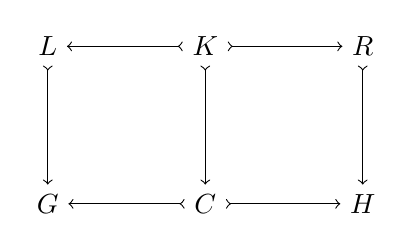
\begin{tikzpicture}
            % [node distance=15mm]
            \node (I) at (0,0) {$K$};
            \node (L)  at (-2,0) {$L$};
            \node (R)  at (2,0) {$R$};
            \node (G)  at (-2,-2) {$G$};
            \node (C)  at (0,-2) {$C$};
            \node (H)  at (2,-2) {$H$};
            \draw [>->] (I) to  node [midway,below] { } (L);
            \draw [>->] (I) to  node [midway,below] { } (R);
            \draw [>->] (L) to node [midway,right] { } (G);
            \draw [>->] (I) to  node [midway,right] 
            % {$u$}
            {} (C);
            \draw [>->] (R) to  node [midway,right]{}
            (H);
            \draw [>->] (C) to node [midway,above] {} (G);
            \draw [>->] (C) to node [midway,above] 
            {}
            (H);
            % \node [at=($(I)!.5!(G)$)] {\normalfont PO};
            % \node [at=($(I)!.5!(H)$)] {\normalfont PO};
        \end{tikzpicture}
    }

    \resizebox{0.8\textwidth}{!}{
            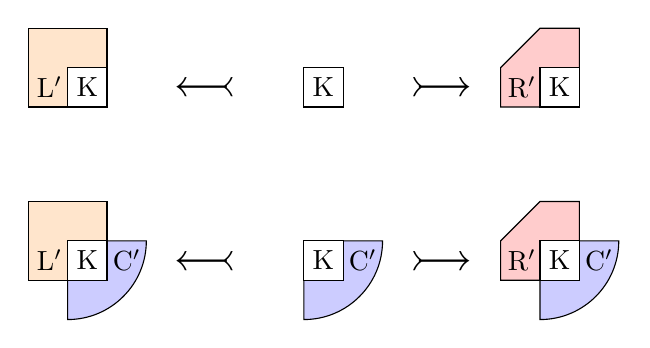
\begin{tikzpicture} 
                \coordinate (k) at (0, 0);
                \draw[fill=white] ($(k)+(0,0)$) rectangle ($(k)+(0.5,0.5)$);
                \node () at ($(k)+(0.25,0.25)$) {\( \mathrm{K} \)};
            
                \coordinate (c) at (0, -2.2);
                \draw[fill=blue!20]
                ($(c)+(0,-0.5)$)
                -- ($(c)+(0,0.5)$) 
                -- ($(c)+(1,0.5)$) 
                arc[start angle=0, end angle=-90, radius=1]
                -- cycle;
                \node () at ($(c)+(0.75,0.25)$) {\( \mathrm{C'} \)};
                \draw[fill=white] ($(c)+(0,0)$) rectangle ($(c)+(0.5,0.5)$);
                \node () at ($(c)+(0.25,0.25)$) {\( \mathrm{K} \)};
            
                \coordinate (l) at (-3, 0);
                \draw[fill=orange!20] ($(l)+(-0.5,0)$) rectangle ($(l)+(0.5,1)$);
                \node () at ($(l)+(-0.23,0.25)$) {\( \mathrm{L'} \)};
                \draw[fill=white] ($(l)+(0,0)$) rectangle ($(l)+(0.5,0.5)$);
                \node () at ($(l)+(0.25,0.25)$) {\( \mathrm{K} \)};
            
                \coordinate (g) at (-3, -2.2);
                \draw[fill=blue!20]
                ($(g)+(0,-0.5)$)
                -- ($(g)+(0,0.5)$)
                -- ($(g)+(1,0.5)$) 
                arc[start angle=0, end angle=-90, radius=1]
                -- cycle;
                \draw[fill=orange!20] ($(g)+(-0.5,0)$) rectangle ($(g)+(0.5,1)$);
                \node () at ($(g)+(0.75,0.25)$) {\( \mathrm{C'} \)};
                \node () at ($(g)+(-0.23,0.25)$) {\( \mathrm{L'} \)};
                \draw[fill=white] ($(g)+(0,0)$) rectangle ($(g)+(0.5,0.5)$);
                \node () at ($(g)+(0.25,0.25)$) {\( \mathrm{K} \)};
            
                \coordinate (r) at (3,0);
                \draw[fill=red!20] ($(r)+(-0.5,0)$)
                -- ($(r)+(-0.5,0.5)$)
                -- ($(r)+(0,1)$)
                --  ($(r)+(0.5,1)$)
                -- ($(r)+(0.5,0)$)
                -- cycle;
                \node () at ($(r)+(-0.23,0.25)$) {\( \mathrm{R'} \)};
                \draw[fill=white] ($(r)+(0,0)$) rectangle ($(r)+(0.5,0.5)$);
                \node () at ($(r)+(0.25,0.25)$) {\( \mathrm{K} \)};
            
                \coordinate (h) at (3, -2.2);
                \draw[fill=blue!20]
                ($(h)+(0,-0.5)$)
                -- ($(h)+(0,0.5)$)
                -- ($(h)+(1,0.5)$) 
                arc[start angle=0, end angle=-90, radius=1]
                -- cycle;
                \draw[fill=red!20] ($(h)+(-0.5,0)$)
                -- ($(h)+(-0.5,0.5)$)
                -- ($(h)+(0,1)$)
                --  ($(h)+(0.5,1)$)
                -- ($(h)+(0.5,0)$)
                -- cycle;
            \node () at ($(h)+(0.75,0.25)$) {\( \mathrm{C'} \)};
            \draw[fill=white] ($(h)+(0,0)$) rectangle ($(h)+(0.5,0.5)$);
            \node () at ($(h)+(0.25,0.25)$) {\( \mathrm{K} \)};
            \node () at ($(h)+(-0.23,0.25)$) {\( \mathrm{R'} \)};
            
                \node[ font=\huge] (kl) at ($(k)!0.5!(l)+(0.25,0.25)$)
            %    {\( \overset{l}{\leftarrowtail} \)}
                {\( \leftarrowtail \)}
                ; 
                \node[ font=\huge] (kr) at ($(k)!0.5!(r)+(0.25,0.25)$)
                {\( \rightarrowtail \)}
                ;  
                \node[ font=\huge] (cg) at ($(c)!0.5!(g)+(0.25,0.25)$) 
                {\( \leftarrowtail \)}
            ;  
                \node[ font=\huge] (ch) at ($(c)!0.5!(h)+(0.25,0.25)$)
                {\( \rightarrowtail \)}
            ; 
                \node[ font=\huge] (kc) at ($(k)!0.5!(c)+(0.2,0.4)$) {\( \downarrowtail \)}; 
            %   \node[ font=\LARGE] () at ($(l)!0.5!(g)+(0.5,0.4)$) {$m$}; 
                \node[ font=\huge] (lg) at ($(l)!0.5!(g)+(0.1,0.4)$) {\( \downarrowtail \)}; 
                \node[ font=\huge] (rh) at ($(r)!0.5!(h)+(0.1,0.4)$) {\( \downarrowtail \)}; 
            %   \node[ font=\LARGE] () at ($(r)!0.5!(h)+(0.55,0.4)$) {$m'$}; 
            %   \node[ font=\LARGE] () at ($(k)!0.5!(c)+(0.5,0.4)$) {$u$}; 
            \end{tikzpicture}
          }
   \end{center}
\end{frame}


\begin{frame}{Analysis of Double-Pushouts Defining Rewriting Steps} 
    \begin{center}
    \resizebox{0.7\textwidth}{!}{
            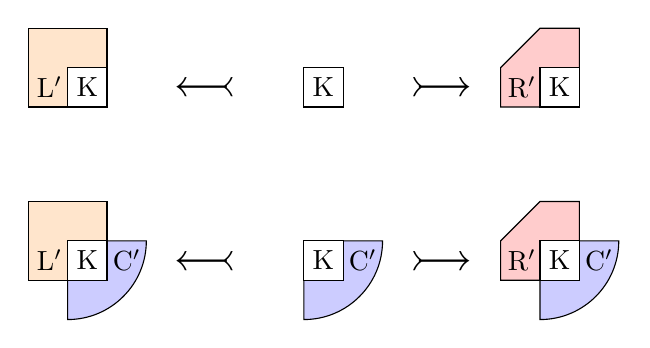
\begin{tikzpicture} 
                \coordinate (k) at (0, 0);
                \draw[fill=white] ($(k)+(0,0)$) rectangle ($(k)+(0.5,0.5)$);
                \node () at ($(k)+(0.25,0.25)$) {\( \mathrm{K} \)};
            
                \coordinate (c) at (0, -2.2);
                \draw[fill=blue!20]
                ($(c)+(0,-0.5)$)
                -- ($(c)+(0,0.5)$) 
                -- ($(c)+(1,0.5)$) 
                arc[start angle=0, end angle=-90, radius=1]
                -- cycle;
                \node () at ($(c)+(0.75,0.25)$) {\( \mathrm{C'} \)};
                \draw[fill=white] ($(c)+(0,0)$) rectangle ($(c)+(0.5,0.5)$);
                \node () at ($(c)+(0.25,0.25)$) {\( \mathrm{K} \)};
            
                \coordinate (l) at (-3, 0);
                \draw[fill=orange!20] ($(l)+(-0.5,0)$) rectangle ($(l)+(0.5,1)$);
                \node () at ($(l)+(-0.23,0.25)$) {\( \mathrm{L'} \)};
                \draw[fill=white] ($(l)+(0,0)$) rectangle ($(l)+(0.5,0.5)$);
                \node () at ($(l)+(0.25,0.25)$) {\( \mathrm{K} \)};
            
                \coordinate (g) at (-3, -2.2);
                \draw[fill=blue!20]
                ($(g)+(0,-0.5)$)
                -- ($(g)+(0,0.5)$)
                -- ($(g)+(1,0.5)$) 
                arc[start angle=0, end angle=-90, radius=1]
                -- cycle;
                \draw[fill=orange!20] ($(g)+(-0.5,0)$) rectangle ($(g)+(0.5,1)$);
                \node () at ($(g)+(0.75,0.25)$) {\( \mathrm{C'} \)};
                \node () at ($(g)+(-0.23,0.25)$) {\( \mathrm{L'} \)};
                \draw[fill=white] ($(g)+(0,0)$) rectangle ($(g)+(0.5,0.5)$);
                \node () at ($(g)+(0.25,0.25)$) {\( \mathrm{K} \)};
            
                \coordinate (r) at (3,0);
                \draw[fill=red!20] ($(r)+(-0.5,0)$)
                -- ($(r)+(-0.5,0.5)$)
                -- ($(r)+(0,1)$)
                --  ($(r)+(0.5,1)$)
                -- ($(r)+(0.5,0)$)
                -- cycle;
                \node () at ($(r)+(-0.23,0.25)$) {\( \mathrm{R'} \)};
                \draw[fill=white] ($(r)+(0,0)$) rectangle ($(r)+(0.5,0.5)$);
                \node () at ($(r)+(0.25,0.25)$) {\( \mathrm{K} \)};
            
                \coordinate (h) at (3, -2.2);
                \draw[fill=blue!20]
                ($(h)+(0,-0.5)$)
                -- ($(h)+(0,0.5)$)
                -- ($(h)+(1,0.5)$) 
                arc[start angle=0, end angle=-90, radius=1]
                -- cycle;
                \draw[fill=red!20] ($(h)+(-0.5,0)$)
                -- ($(h)+(-0.5,0.5)$)
                -- ($(h)+(0,1)$)
                --  ($(h)+(0.5,1)$)
                -- ($(h)+(0.5,0)$)
                -- cycle;
            \node () at ($(h)+(0.75,0.25)$) {\( \mathrm{C'} \)};
            \draw[fill=white] ($(h)+(0,0)$) rectangle ($(h)+(0.5,0.5)$);
            \node () at ($(h)+(0.25,0.25)$) {\( \mathrm{K} \)};
            \node () at ($(h)+(-0.23,0.25)$) {\( \mathrm{R'} \)};
            
                \node[ font=\huge] (kl) at ($(k)!0.5!(l)+(0.25,0.25)$)
            %    {\( \overset{l}{\leftarrowtail} \)}
                {\( \leftarrowtail \)}
                ; 
                \node[ font=\huge] (kr) at ($(k)!0.5!(r)+(0.25,0.25)$)
                {\( \rightarrowtail \)}
                ;  
                \node[ font=\huge] (cg) at ($(c)!0.5!(g)+(0.25,0.25)$) 
                {\( \leftarrowtail \)}
            ;  
                \node[ font=\huge] (ch) at ($(c)!0.5!(h)+(0.25,0.25)$)
                {\( \rightarrowtail \)}
            ; 
                \node[ font=\huge] (kc) at ($(k)!0.5!(c)+(0.2,0.4)$) {\( \downarrowtail \)}; 
            %   \node[ font=\LARGE] () at ($(l)!0.5!(g)+(0.5,0.4)$) {$m$}; 
                \node[ font=\huge] (lg) at ($(l)!0.5!(g)+(0.1,0.4)$) {\( \downarrowtail \)}; 
                \node[ font=\huge] (rh) at ($(r)!0.5!(h)+(0.1,0.4)$) {\( \downarrowtail \)}; 
            %   \node[ font=\LARGE] () at ($(r)!0.5!(h)+(0.55,0.4)$) {$m'$}; 
            %   \node[ font=\LARGE] () at ($(k)!0.5!(c)+(0.5,0.4)$) {$u$}; 
            \end{tikzpicture}
          }
   \end{center}

   Example
    \begin{center}
    \resizebox{0.8\textwidth}{!}{
      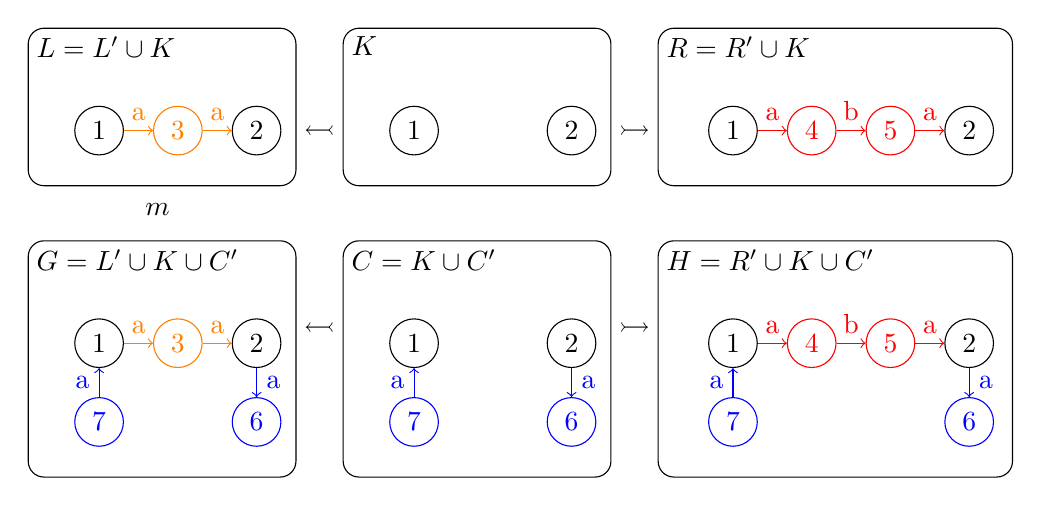
\begin{tikzpicture}
              \graphbox{\( L = L' \cup K \)}{0mm}{5mm}{34mm}{20mm}{2mm}{-5mm}{
                  \coordinate (o) at (0mm,-8mm); 
                  \node[draw,circle] (l1) at ($(o)+(-10mm,0mm)$) {1};
                  \node[draw,circle] (l2) at ($(l1)+(2,0)$) {2};
                  \node[orange,draw,circle] (l3) at ($(l1) + (1,0)$) {3};
                  \draw[orange,->] (l1) -- (l3) node[midway,above] {a};
                  \draw[orange,->] (l3) -- (l2) node[midway,above] {a};
              } 

              \graphbox{\( K \)}{40mm}{5mm}{34mm}{20mm}{2mm}{-5mm}{
                  \coordinate (o) at (0mm,-8mm); 
                  \node[draw,circle] (l1) at ($(o)+(-10mm,0mm)$) {1};
                  \node[draw,circle] (l2) at ($(l1)+(2,0)$) {2};
              }  

              \graphbox{\( R = R' \cup K \)}{80mm}{5mm}{45mm}{20mm}{2mm}{-5mm}{
                  \coordinate (o) at (-5mm,-8mm); 
                  \node[draw,circle] (l1) at ($(o)+(-10mm,0mm)$) {1};
                  \node[draw,circle] (l2) at ($(l1)+(3,0)$) {2};
                  \node[red,draw,circle] (l3) at ($(l1) + (1,0)$) {4};
                  \node[red,draw,circle] (l4) at ($(l1) + (2,0)$) {5};
                  \draw[red,->] (l1) -- (l3) node[midway,above] {a};
                  \draw[red,->] (l3) -- (l4) node[midway,above] {b};
                  \draw[red,->] (l4) -- (l2) node[midway,above] {a};
              }    

              \graphbox{\( G = L' \cup K \cup C' \)}{0mm}{-22mm}{34mm}{30mm}{2mm}{-10mm}{
                  \coordinate (o) at (0mm,-3mm); 
                  \node[draw,circle] (l1) at ($(o)+(-10mm,0mm)$) {1};
                  \node[draw,circle] (l2) at ($(l1)+(2,0)$) {2};
                  \node[draw,circle,orange] (l3) at ($(l1) + (1,0)$) {3};
                  \node[blue, draw,circle] (l4) at ($(l2) + (0,-1)$) {6};
                  \draw[orange,->] (l1) -- (l3) node[midway,above] {a};
                  \draw[orange,->] (l3) -- (l2) node[midway,above] {a};
                  \draw[blue,->] (l2) -- (l4) node[midway,right] {a};
                  \node[blue,draw,circle] (l6) at ($(l1) + (0,-1)$) {7};
                  \draw[blue,<-] (l1) -- (l6) node[midway,left] {a};
              }    

              \graphbox{\( C = K \cup C' \)}{40mm}{-22mm}{34mm}{30mm}{2mm}{-10mm}{
                  \coordinate (o) at (0mm,-3mm); 
                  \node[draw,circle] (l1) at ($(o)+(-10mm,0mm)$) {1};
                  \node[draw,circle] (l2) at ($(l1)+(2,0)$) {2};
                  \node[blue,draw,circle] (l4) at ($(l2) + (0,-1)$) {6};
                  \draw[blue,->] (l2) -- (l4) node[midway,right] {a};
                  \node[blue,draw,circle] (l6) at ($(l1) + (0,-1)$) {7};
                  \draw[blue,<-] (l1) -- (l6) node[midway,left] {a};
              }    

              \graphbox{\( H = R' \cup K \cup C' \)}{80mm}{-22mm}{45mm}{30mm}{2mm}{-10mm}{
                  \coordinate (o) at (-5mm,-3mm); 
                  \node[draw,circle] (l1) at ($(o)+(-10mm,0mm)$) {1};
                  \node[draw,circle] (l2) at ($(l1)+(3,0)$) {2};
                  \node[draw,circle,red] (l3) at ($(l1) + (1,0)$) {4};
                  \node[draw,circle,red] (l4) at ($(l1) + (2,0)$) {5};
                  \node[blue,draw,circle] (l5) at ($(l2) + (0,-1)$) {6};
                  \node[blue,draw,circle] (l6) at ($(l1) + (0,-1)$) {7};
                  \draw[blue,<-] (l1) -- (l6) node[midway,left] {a};
                  \draw[red,->] (l1) -- (l3) node[midway,above] {a};
                  \draw[red,->] (l3) -- (l4) node[midway,above] {b};
                  \draw[red,->] (l4) -- (l2) node[midway,above] {a};
                  \draw[blue,->] (l2) -- (l5) node[midway,right] {a};
              }    

              \node () at (37mm,-8mm) {\( \leftarrowtail \)}; % K -> L
              \node () at (77mm,-8mm) {\( \rightarrowtail \)}; % K -> R
              \node () at (17mm,-18mm) {\( m\ \downarrowtail \)};
              \node () at (37mm,-33mm) {\( \leftarrowtail \)};
              \node () at (52mm,-18mm) {\( \downarrowtail \)};
              \node () at (92mm,-18mm) {\( \downarrowtail \)};
              \node () at (77mm,-33mm) {\( \rightarrowtail \)}; % C -> H
      \end{tikzpicture}
      }
   \end{center}
\end{frame}


% \begin{frame}{Occurrences}
%     $X, G$ : graphs\\
%     An \textcolor{red}{$X$-occurrence} in $G$ is a \textcolor{red}{subgraph} of $G$ isomorphic to $X$.\\
% \end{frame}

% \begin{frame}{Implicit creation and deletion of subgraphs}
%     A DPO diagram witnessing a rewriting step:

%     \resizebox{0.7\textwidth}{!}{
%             \begin{tikzpicture}
%                 \coordinate (k) at (0, 0);
%                 \draw[fill=white] ($(k)+(0,0)$) rectangle ($(k)+(0.5,0.5)$);
%                 \node () at ($(k)+(0.25,0.25)$) {\( \mathrm{K} \)};
            
%                 \coordinate (c) at (0, -2.2);
%                 \draw[fill=blue!20]
%                 ($(c)+(0,-0.5)$)
%                 -- ($(c)+(0,0.5)$) 
%                 -- ($(c)+(1,0.5)$) 
%                 arc[start angle=0, end angle=-90, radius=1]
%                 -- cycle;
%                 \node () at ($(c)+(0.75,0.25)$) {\( \mathrm{C'} \)};
%                 \draw[fill=white] ($(c)+(0,0)$) rectangle ($(c)+(0.5,0.5)$);
%                 \node () at ($(c)+(0.25,0.25)$) {\( \mathrm{K} \)};
            
%                 \coordinate (l) at (-3, 0);
%                 \draw[fill=orange!20] ($(l)+(-0.5,0)$) rectangle ($(l)+(0.5,1)$);
%                 \node () at ($(l)+(-0.23,0.25)$) {\( \mathrm{L'} \)};
%                 \draw[fill=white] ($(l)+(0,0)$) rectangle ($(l)+(0.5,0.5)$);
%                 \node () at ($(l)+(0.25,0.25)$) {\( \mathrm{K} \)};
            
%                 \coordinate (g) at (-3, -2.2);
%                 \draw[fill=blue!20]
%                 ($(g)+(0,-0.5)$)
%                 -- ($(g)+(0,0.5)$)
%                 -- ($(g)+(1,0.5)$) 
%                 arc[start angle=0, end angle=-90, radius=1]
%                 -- cycle;
%                 \draw[fill=orange!20] ($(g)+(-0.5,0)$) rectangle ($(g)+(0.5,1)$);
%                 \node () at ($(g)+(0.75,0.25)$) {\( \mathrm{C'} \)};
%                 \node () at ($(g)+(-0.23,0.25)$) {\( \mathrm{L'} \)};
%                 \draw[fill=white] ($(g)+(0,0)$) rectangle ($(g)+(0.5,0.5)$);
%                 \node () at ($(g)+(0.25,0.25)$) {\( \mathrm{K} \)};
            
%                 \coordinate (r) at (3,0);
%                 \draw[fill=red!20] ($(r)+(-0.5,0)$)
%                 -- ($(r)+(-0.5,0.5)$)
%                 -- ($(r)+(0,1)$)
%                 --  ($(r)+(0.5,1)$)
%                 -- ($(r)+(0.5,0)$)
%                 -- cycle;
%                 \node () at ($(r)+(-0.23,0.25)$) {\( \mathrm{R'} \)};
%                 \draw[fill=white] ($(r)+(0,0)$) rectangle ($(r)+(0.5,0.5)$);
%                 \node () at ($(r)+(0.25,0.25)$) {\( \mathrm{K} \)};
            
%                 \coordinate (h) at (3, -2.2);
%                 \draw[fill=blue!20]
%                 ($(h)+(0,-0.5)$)
%                 -- ($(h)+(0,0.5)$)
%                 -- ($(h)+(1,0.5)$) 
%                 arc[start angle=0, end angle=-90, radius=1]
%                 -- cycle;
%                 \draw[fill=red!20] ($(h)+(-0.5,0)$)
%                 -- ($(h)+(-0.5,0.5)$)
%                 -- ($(h)+(0,1)$)
%                 --  ($(h)+(0.5,1)$)
%                 -- ($(h)+(0.5,0)$)
%                 -- cycle;
%             \node () at ($(h)+(0.75,0.25)$) {\( \mathrm{C'} \)};
%             \draw[fill=white] ($(h)+(0,0)$) rectangle ($(h)+(0.5,0.5)$);
%             \node () at ($(h)+(0.25,0.25)$) {\( \mathrm{K} \)};
%             \node () at ($(h)+(-0.23,0.25)$) {\( \mathrm{R'} \)};
            
%                 \node[ font=\huge] (kl) at ($(k)!0.5!(l)+(0.25,0.25)$)
%             %    {\( \overset{l}{\leftarrowtail} \)}
%                 {\( \leftarrowtail \)}
%                 ; 
%                 \node[ font=\huge] (kr) at ($(k)!0.5!(r)+(0.25,0.25)$)
%                 {\( \rightarrowtail \)}
%                 ;  
%                 \node[ font=\huge] (cg) at ($(c)!0.5!(g)+(0.25,0.25)$) 
%                 {\( \leftarrowtail \)}
%             ;  
%                 \node[ font=\huge] (ch) at ($(c)!0.5!(h)+(0.25,0.25)$)
%                 {\( \rightarrowtail \)}
%             ; 
%                 \node[ font=\huge] (kc) at ($(k)!0.5!(c)+(0.2,0.4)$) {\( \downarrowtail \)}; 
%             %   \node[ font=\LARGE] () at ($(l)!0.5!(g)+(0.5,0.4)$) {$m$}; 
%                 \node[ font=\huge] (lg) at ($(l)!0.5!(g)+(0.1,0.4)$) {\( \downarrowtail \)}; 
%                 \node[ font=\huge] (rh) at ($(r)!0.5!(h)+(0.1,0.4)$) {\( \downarrowtail \)}; 
%             %   \node[ font=\LARGE] () at ($(r)!0.5!(h)+(0.55,0.4)$) {$m'$}; 
%             %   \node[ font=\LARGE] () at ($(k)!0.5!(c)+(0.5,0.4)$) {$u$}; 
%             \end{tikzpicture}
%           }

%     An occurrence $x$ of a graph $X$ is 
%     \begin{itemize}
%         \item \textcolor{red}{explicitly deleted} if $x \subseteq L' \cup K$ 
%         \item \textcolor{blue}{explicitly created} if $x \subseteq R' \cup K$
%         \item \hspace{1.57cm} shared if $x \subseteq C' \cup K$
%         \item \textcolor{red}{implicitly deleted} if $x \not \subseteq L' \cup K$ and $x \not \subseteq C' \cup K$
%         \item \textcolor{blue}{implicitly created} if $x \not \subseteq R' \cup K$ and $x \not \subseteq C' \cup K$
%     \end{itemize}

% \end{frame}



% \begin{frame}{Explicit occurrences}
%     Rule : $L \overset{l}{\leftarrowtail} K \overset{r}{\rightarrowtail} R$

%     Rewriting step :

%     \resizebox{0.5\textwidth}{!}{
%         \begin{tikzpicture}
%             % [node distance=15mm]
%             \node (I) at (0,0) {K};
%             \node (L)  at (-2,0) {L};
%             \node (R)  at (2,0) {R};
%             \node (G)  at (-2,-2) {G};
%             \node (C)  at (0,-2) {C};
%             \node (H)  at (2,-2) {H};
%             \draw [>->] (I) to  node [midway,above] {l} (L);
%             \draw [>->] (I) to  node [midway,above] {r} (R);
%             \draw [>->] (L) to node [midway,left] {m} (G);
%             \draw [>->] (I) to (C);
%             \draw [>->] (R) to (H);
%             \draw [>->] (C) to (G);
%             \draw [>->] (C) to (H); 
%         \end{tikzpicture}
%     }
    
%     $X$ : graph 

%     An $X$-occurrence is 
%     \begin{itemize} 
%         \item \textcolor{red}{explicit} if it is included in $L' \cup K$ or $x \subseteq R' \cup K$ 
%         \item \textcolor{red}{implicit} if $x \not \subseteq L' \cup K$ and $x \not \subseteq C' \cup K$
%         \item \textcolor{blue}{implicitly} otherwise
%     \end{itemize}
    

% \end{frame}

\begin{frame}{Implicit, Explicit and Shared Occurrences}
  
    An \textcolor{red}{$X$-occurrence} in $G$ is a \textcolor{red}{subgraph} of $G$ isomorphic to $X$. 

    % A DPO diagram witnessing a rewriting step:
 \begin{center}
       \resizebox{0.49\textwidth}{!}{
        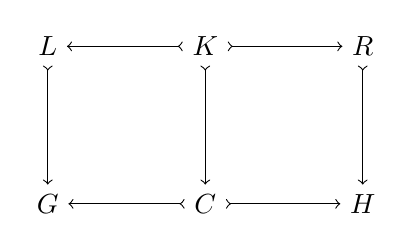
\begin{tikzpicture}
            % [node distance=15mm]
            \node (I) at (0,0) {$K$};
            \node (L)  at (-2,0) {$L$};
            \node (R)  at (2,0) {$R$};
            \node (G)  at (-2,-2) {$G$};
            \node (C)  at (0,-2) {$C$};
            \node (H)  at (2,-2) {$H$};
            \draw [>->] (I) to  node [midway,below] { } (L);
            \draw [>->] (I) to  node [midway,below] { } (R);
            \draw [>->] (L) to node [midway,right] { } (G);
            \draw [>->] (I) to  node [midway,right] 
            % {$u$}
            {} (C);
            \draw [>->] (R) to  node [midway,right] 
            {}
            (H);
            \draw [>->] (C) to node [midway,above] {} (G);
            \draw [>->] (C) to node [midway,above] 
            {}
            (H);
            % \node [at=($(I)!.5!(G)$)] {\normalfont PO};
            % \node [at=($(I)!.5!(H)$)] {\normalfont PO};
        \end{tikzpicture}
    }
    \resizebox{0.49\textwidth}{!}{
            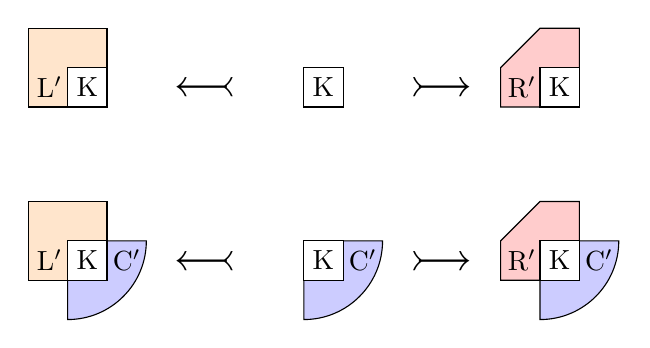
\begin{tikzpicture} 
                \coordinate (k) at (0, 0);
                \draw[fill=white] ($(k)+(0,0)$) rectangle ($(k)+(0.5,0.5)$);
                \node () at ($(k)+(0.25,0.25)$) {\( \mathrm{K} \)};
            
                \coordinate (c) at (0, -2.2);
                \draw[fill=blue!20]
                ($(c)+(0,-0.5)$)
                -- ($(c)+(0,0.5)$) 
                -- ($(c)+(1,0.5)$) 
                arc[start angle=0, end angle=-90, radius=1]
                -- cycle;
                \node () at ($(c)+(0.75,0.25)$) {\( \mathrm{C'} \)};
                \draw[fill=white] ($(c)+(0,0)$) rectangle ($(c)+(0.5,0.5)$);
                \node () at ($(c)+(0.25,0.25)$) {\( \mathrm{K} \)};
            
                \coordinate (l) at (-3, 0);
                \draw[fill=orange!20] ($(l)+(-0.5,0)$) rectangle ($(l)+(0.5,1)$);
                \node () at ($(l)+(-0.23,0.25)$) {\( \mathrm{L'} \)};
                \draw[fill=white] ($(l)+(0,0)$) rectangle ($(l)+(0.5,0.5)$);
                \node () at ($(l)+(0.25,0.25)$) {\( \mathrm{K} \)};
            
                \coordinate (g) at (-3, -2.2);
                \draw[fill=blue!20]
                ($(g)+(0,-0.5)$)
                -- ($(g)+(0,0.5)$)
                -- ($(g)+(1,0.5)$) 
                arc[start angle=0, end angle=-90, radius=1]
                -- cycle;
                \draw[fill=orange!20] ($(g)+(-0.5,0)$) rectangle ($(g)+(0.5,1)$);
                \node () at ($(g)+(0.75,0.25)$) {\( \mathrm{C'} \)};
                \node () at ($(g)+(-0.23,0.25)$) {\( \mathrm{L'} \)};
                \draw[fill=white] ($(g)+(0,0)$) rectangle ($(g)+(0.5,0.5)$);
                \node () at ($(g)+(0.25,0.25)$) {\( \mathrm{K} \)};
            
                \coordinate (r) at (3,0);
                \draw[fill=red!20] ($(r)+(-0.5,0)$)
                -- ($(r)+(-0.5,0.5)$)
                -- ($(r)+(0,1)$)
                --  ($(r)+(0.5,1)$)
                -- ($(r)+(0.5,0)$)
                -- cycle;
                \node () at ($(r)+(-0.23,0.25)$) {\( \mathrm{R'} \)};
                \draw[fill=white] ($(r)+(0,0)$) rectangle ($(r)+(0.5,0.5)$);
                \node () at ($(r)+(0.25,0.25)$) {\( \mathrm{K} \)};
            
                \coordinate (h) at (3, -2.2);
                \draw[fill=blue!20]
                ($(h)+(0,-0.5)$)
                -- ($(h)+(0,0.5)$)
                -- ($(h)+(1,0.5)$) 
                arc[start angle=0, end angle=-90, radius=1]
                -- cycle;
                \draw[fill=red!20] ($(h)+(-0.5,0)$)
                -- ($(h)+(-0.5,0.5)$)
                -- ($(h)+(0,1)$)
                --  ($(h)+(0.5,1)$)
                -- ($(h)+(0.5,0)$)
                -- cycle;
            \node () at ($(h)+(0.75,0.25)$) {\( \mathrm{C'} \)};
            \draw[fill=white] ($(h)+(0,0)$) rectangle ($(h)+(0.5,0.5)$);
            \node () at ($(h)+(0.25,0.25)$) {\( \mathrm{K} \)};
            \node () at ($(h)+(-0.23,0.25)$) {\( \mathrm{R'} \)};
            
                \node[ font=\huge] (kl) at ($(k)!0.5!(l)+(0.25,0.25)$)
            %    {\( \overset{l}{\leftarrowtail} \)}
                {\( \leftarrowtail \)}
                ; 
                \node[ font=\huge] (kr) at ($(k)!0.5!(r)+(0.25,0.25)$)
                {\( \rightarrowtail \)}
                ;  
                \node[ font=\huge] (cg) at ($(c)!0.5!(g)+(0.25,0.25)$) 
                {\( \leftarrowtail \)}
            ;  
                \node[ font=\huge] (ch) at ($(c)!0.5!(h)+(0.25,0.25)$)
                {\( \rightarrowtail \)}
            ; 
                \node[ font=\huge] (kc) at ($(k)!0.5!(c)+(0.2,0.4)$) {\( \downarrowtail \)}; 
            %   \node[ font=\LARGE] () at ($(l)!0.5!(g)+(0.5,0.4)$) {$m$}; 
                \node[ font=\huge] (lg) at ($(l)!0.5!(g)+(0.1,0.4)$) {\( \downarrowtail \)}; 
                \node[ font=\huge] (rh) at ($(r)!0.5!(h)+(0.1,0.4)$) {\( \downarrowtail \)}; 
            %   \node[ font=\LARGE] () at ($(r)!0.5!(h)+(0.55,0.4)$) {$m'$}; 
            %   \node[ font=\LARGE] () at ($(k)!0.5!(c)+(0.5,0.4)$) {$u$}; 
            \end{tikzpicture}
          }
   \end{center}

    $X$ : a subgraph of $L$

    $X$-occurrence $y$ in $G$ is 

    \parbox{0.45\textwidth}{\hspace{3mm}$\bullet$ \textcolor{red}{shared} if $y \subseteq C$}
    \parbox{0.45\textwidth}{\hspace{3mm}$\bullet$ \textcolor{red}{explicit} if $y \subseteq L$}

    \parbox{\textwidth}{\hspace{3mm}$\bullet$ \textcolor{red}{implicit} if $y \cap C' \neq \emptyset$ and \textcolor{blue}{$y \cap L' \neq  \emptyset$}}

    % \begin{itemize} 
    %     % \item \textcolor{red}{shared} if $y \subseteq C$ 
    %     % \item \textcolor{red}{explicit} if $y \subseteq L$  
    %     \item \textcolor{red}{implicit} if $y \cap C' \neq \emptyset$ and \textcolor{blue}{$y \cap L' \neq  \emptyset$}
    %     % if $y \not \subseteq L' \cup K$ and $y \not \subseteq C' \cup K$
    % \end{itemize}
    
    $X$-occurrence $y$ in $H$ is 

   \parbox{0.45\textwidth}{\hspace{3mm}$\bullet$ \textcolor{red}{shared} if $y \subseteq C$}
   \parbox{0.45\textwidth}{\hspace{3mm}$\bullet$ \textcolor{red}{explicit} if $y \subseteq R$ }

    \parbox{\textwidth}{\hspace{3mm}$\bullet$ \textcolor{red}{implicit} if $y \cap C' \neq \emptyset$ and \textcolor{blue}{$y \cap R' \neq \emptyset$}}
    % \begin{itemize} 
    %     % \item \textcolor{red}{explicit} if $y \subseteq K \cup L'$ or $y \subseteq K \cup R'$ 
    %     % \item \textcolor{red}{explicit} if $y \subseteq L$ or $y \subseteq R$ 
    %     % \item \textcolor{red}{shared} if $y \subseteq C$
    %     % \item \textcolor{red}{implicit} otherwise (i.e. $y \cap C' \neq \emptyset$, and $y \cap L' \neq  \emptyset$ or $y \cap R' \neq \emptyset$)
    %     \item \textcolor{red}{shared} if $y \subseteq C$
    %     \item \textcolor{red}{explicit} if $y \subseteq R$ 
    %     \item \textcolor{red}{implicit} if $y \cap C' \neq \emptyset$ and \textcolor{blue}{$y \cap R' \neq \emptyset$}
    %     % if $y \not \subseteq L' \cup K$ and $y \not \subseteq C' \cup K$
    % \end{itemize}
\end{frame}
 

\begin{frame}{Implicitly created and deleted occurrences: example}

   \begin{center}
    \resizebox{0.9\textwidth}{!}{
      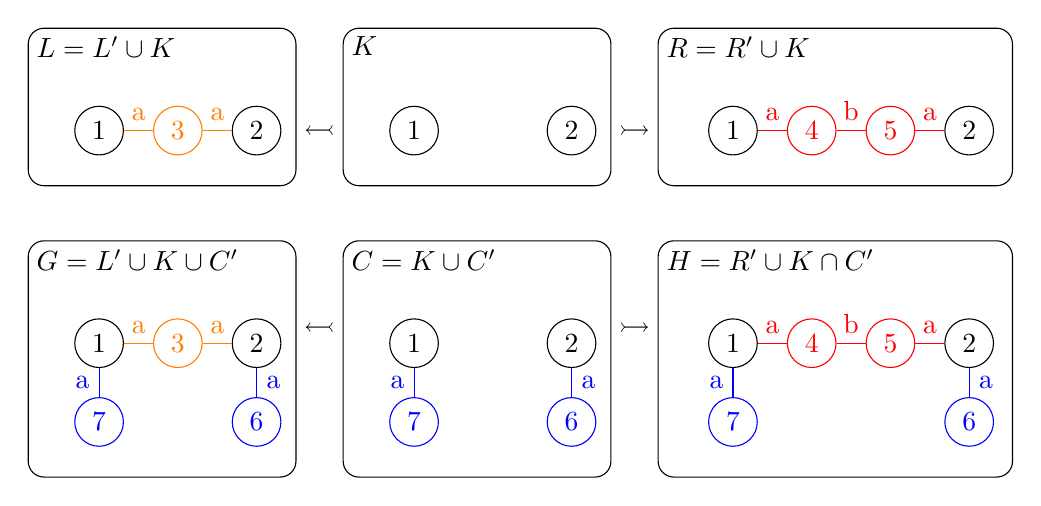
\begin{tikzpicture}
              \graphbox{\( L = L' \cup K \)}{0mm}{5mm}{34mm}{20mm}{2mm}{-5mm}{
                  \coordinate (o) at (0mm,-8mm); 
                  \node[draw,circle] (l1) at ($(o)+(-10mm,0mm)$) {1};
                  \node[draw,circle] (l2) at ($(l1)+(2,0)$) {2};
                  \node[orange,draw,circle] (l3) at ($(l1) + (1,0)$) {3};
                  \draw[orange] (l1) -- (l3) node[midway,above] {a};
                  \draw[orange] (l3) -- (l2) node[midway,above] {a};
              } 

              \graphbox{\( K \)}{40mm}{5mm}{34mm}{20mm}{2mm}{-5mm}{
                  \coordinate (o) at (0mm,-8mm); 
                  \node[draw,circle] (l1) at ($(o)+(-10mm,0mm)$) {1};
                  \node[draw,circle] (l2) at ($(l1)+(2,0)$) {2};
              }  

              \graphbox{\( R = R' \cup K \)}{80mm}{5mm}{45mm}{20mm}{2mm}{-5mm}{
                  \coordinate (o) at (-5mm,-8mm); 
                  \node[draw,circle] (l1) at ($(o)+(-10mm,0mm)$) {1};
                  \node[draw,circle] (l2) at ($(l1)+(3,0)$) {2};
                  \node[red,draw,circle] (l3) at ($(l1) + (1,0)$) {4};
                  \node[red,draw,circle] (l4) at ($(l1) + (2,0)$) {5};
                  \draw[red] (l1) -- (l3) node[midway,above] {a};
                  \draw[red] (l3) -- (l4) node[midway,above] {b};
                  \draw[red] (l4) -- (l2) node[midway,above] {a};
              }    

              \graphbox{\( G = L' \cup K \cup C' \)}{0mm}{-22mm}{34mm}{30mm}{2mm}{-10mm}{
                  \coordinate (o) at (0mm,-3mm); 
                  \node[draw,circle] (l1) at ($(o)+(-10mm,0mm)$) {1};
                  \node[draw,circle] (l2) at ($(l1)+(2,0)$) {2};
                  \node[draw,circle,orange] (l3) at ($(l1) + (1,0)$) {3};
                  \node[blue, draw,circle] (l4) at ($(l2) + (0,-1)$) {6};
                  \draw[orange] (l1) -- (l3) node[midway,above] {a};
                  \draw[orange] (l3) -- (l2) node[midway,above] {a};
                  \draw[blue] (l2) -- (l4) node[midway,right] {a};
                  \node[blue,draw,circle] (l6) at ($(l1) + (0,-1)$) {7};
                  \draw[blue] (l1) -- (l6) node[midway,left] {a};
              }    

              \graphbox{\( C = K \cup C' \)}{40mm}{-22mm}{34mm}{30mm}{2mm}{-10mm}{
                  \coordinate (o) at (0mm,-3mm); 
                  \node[draw,circle] (l1) at ($(o)+(-10mm,0mm)$) {1};
                  \node[draw,circle] (l2) at ($(l1)+(2,0)$) {2};
                  \node[blue,draw,circle] (l4) at ($(l2) + (0,-1)$) {6};
                  \draw[blue] (l2) -- (l4) node[midway,right] {a};
                  \node[blue,draw,circle] (l6) at ($(l1) + (0,-1)$) {7};
                  \draw[blue] (l1) -- (l6) node[midway,left] {a};
              }    

              \graphbox{\( H = R' \cup K \cap C' \)}{80mm}{-22mm}{45mm}{30mm}{2mm}{-10mm}{
                  \coordinate (o) at (-5mm,-3mm); 
                  \node[draw,circle] (l1) at ($(o)+(-10mm,0mm)$) {1};
                  \node[draw,circle] (l2) at ($(l1)+(3,0)$) {2};
                  \node[draw,circle,red] (l3) at ($(l1) + (1,0)$) {4};
                  \node[draw,circle,red] (l4) at ($(l1) + (2,0)$) {5};
                  \node[blue,draw,circle] (l5) at ($(l2) + (0,-1)$) {6};
                  \node[blue,draw,circle] (l6) at ($(l1) + (0,-1)$) {7};
                  \draw[blue] (l1) -- (l6) node[midway,left] {a};
                  \draw[red] (l1) -- (l3) node[midway,above] {a};
                  \draw[red] (l3) -- (l4) node[midway,above] {b};
                  \draw[red] (l4) -- (l2) node[midway,above] {a};
                  \draw[blue] (l2) -- (l5) node[midway,right] {a};
              }    

              \node () at (37mm,-8mm) {\( \leftarrowtail \)}; % K -> L
              \node () at (77mm,-8mm) {\( \rightarrowtail \)}; % K -> R
              \node () at (17mm,-18mm) {\( \downarrowtail \)};
              \node () at (37mm,-33mm) {\( \leftarrowtail \)};
              \node () at (52mm,-18mm) {\( \downarrowtail \)};
              \node () at (92mm,-18mm) {\( \downarrowtail \)};
              \node () at (77mm,-33mm) {\( \rightarrowtail \)}; % C -> H
      \end{tikzpicture}
      }
   \end{center}

   Graph \tikz[baseline=-0.5ex]{ 
        \node (x) at (0,0) {$\bullet$};  
        \node (y) at (1,0) {$\bullet$};
        \node (z) at (2,0) {$\bullet$};
        \draw[->] (x) -- node[midway,below] {a} (y) ;
        \draw[->] (y) -- node[midway,below] {a} (z) ;
    }

        No shared occurrences.

        1 explicit occurrence in $G$: 1-3-2 

        0 explicit occurrence in $H$
    
        2 implicit occurrences in $G$: 7-1-3, 3-2-6 
        
        2 implicit occurrences in $H$: 7-1-4, 5-2-6 
\end{frame}


\begin{frame}{$X$-occurrences in a graph $G$}
    Remark:

    \begin{flalign*}
     \mathop{\mid}\text{$X$-occurrences}\mathop{\mid} =
            &\mathop{\mid}\text{explicit $X$-occurrences}\mathop{\mid} \mathop{+} \\
            &\mathop{\mid}\text{shared $X$-occurrences}\mathop{\mid} \mathop{+} \\
            &\mathop{\mid}\text{implicit $X$-occurrences}\mathop{\mid}
    \end{flalign*}
\end{frame} 

\begin{frame}{Termination of a graph rewriting rule $\varphi$}
    \begin{itemize}
        \item $X$: a subgraph of $\opn{lhs}(\varphi)$
        \item $\varphi$ terminates if for all $G \Rightarrow_\varphi H$, the number of $X$-occurrences strictly decreases.
            % \begin{flalign*}
            % &\mathop{\mid}\text{$X$-occurrences in $G$}\mathop{\mid} - \mathop{\mid}\text{$X$-occurrences in $H$}\mathop{\mid} \\
            % % = &\mathop{\mid}\text{explicit $X$-occurrences in $G$}\mathop{\mid} - \mathop{\mid}\text{explicit $X$-occurrences in $H$}\mathop{\mid}  +\\
            % %         &\mathop{\mid}\text{implicit $X$-occurrences in $G$}\mathop{\mid} - \mathop{\mid}\text{implicit $X$-occurrences in $H$}\mathop{\mid} \\
            % \mathop{>} & 0
            % \end{flalign*}
            % because $\text{shared $X$-occurrences in $G$} = \text{shared $X$-occurrences in $H$}$.
        \item $\varphi$ terminates if for all $G \Rightarrow_\varphi H$,  
            \begin{flalign*}
            &\mathop{\mid}\text{explicit $X$-occurrences in $G$}\mathop{\mid} \mathop{-} \mathop{\mid}\text{explicit $X$-occurrences in $H$}\mathop{\mid}  \mathop{+}\\
                    &\mathop{\mid}\text{implicit $X$-occurrences in $G$}\mathop{\mid} \mathop{-} \mathop{\mid}\text{implicit $X$-occurrences in $H$}\mathop{\mid} \\
            &\mathop{>} 0
            \end{flalign*}
            because $G$ and $H$ shared the same shared $X$-occurrences.
        \item $\varphi$ terminates if for all $G \Rightarrow H$,
        \begin{flalign*}
            &\mathop{\mid}\text{explicit $X$-occurrences in $G$}\mathop{\mid} \mathop{>} \mathop{\mid}\text{explicit $X$-occurrences in $H$}\mathop{\mid} \\
            &\mathop{\mid}\text{implicit $X$-occurrences in $G$}\mathop{\mid} \mathop{\geq} \mathop{\mid}\text{implicit $X$-occurrences in $H$}\mathop{\mid} 
        \end{flalign*}
    \end{itemize}
    
 
    

   
\end{frame}

\begin{frame}{Termination of a graph rewriting rule}


   

    The first condition 
    $$\mathop{\mid}\text{explicit $X$-occurrences in $G$}\mathop{\mid} \mathop{>} \mathop{\mid}\text{explicit $X$-occurrences in $H$}\mathop{\mid}$$
    
    is equivalent to 
        \begin{flalign*}
        \mathop{\mid}\text{$X$-occurrences in $L$}\mathop{\mid} \mathop{>} \mathop{\mid}\text{$X$-occurrences in $R$}\mathop{\mid} 
    \end{flalign*}


    \begin{center}
    %     \resizebox{0.49\textwidth}{!}{
    %     \begin{tikzpicture}
    %         % [node distance=15mm]
    %         \node (I) at (0,0) {$K$};
    %         \node (L)  at (-2,0) {$L$};
    %         \node (R)  at (2,0) {$R$};
    %         \node (G)  at (-2,-2) {$G$};
    %         \node (C)  at (0,-2) {$C$};
    %         \node (H)  at (2,-2) {$H$};
    %         \draw [>->] (I) to  node [midway,below] { } (L);
    %         \draw [>->] (I) to  node [midway,below] { } (R);
    %         \draw [>->] (L) to node [midway,right] { } (G);
    %         \draw [>->] (I) to  node [midway,right] 
    %         % {$u$}
    %         {} (C);
    %         \draw [>->] (R) to  node [midway,right] 
    %         {$m'$}
    %         (H);
    %         \draw [>->] (C) to node [midway,above] {} (G);
    %         \draw [>->] (C) to node [midway,above] 
    %         {}
    %         (H);
    %         % \node [at=($(I)!.5!(G)$)] {\normalfont PO};
    %         % \node [at=($(I)!.5!(H)$)] {\normalfont PO};
    %     \end{tikzpicture}
    % }
    \resizebox{0.6\textwidth}{!}{
            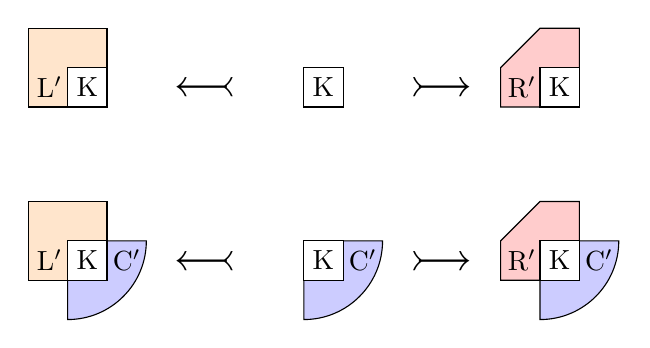
\begin{tikzpicture} 
                \coordinate (k) at (0, 0);
                \draw[fill=white] ($(k)+(0,0)$) rectangle ($(k)+(0.5,0.5)$);
                \node () at ($(k)+(0.25,0.25)$) {\( \mathrm{K} \)};
            
                \coordinate (c) at (0, -2.2);
                \draw[fill=blue!20]
                ($(c)+(0,-0.5)$)
                -- ($(c)+(0,0.5)$) 
                -- ($(c)+(1,0.5)$) 
                arc[start angle=0, end angle=-90, radius=1]
                -- cycle;
                \node () at ($(c)+(0.75,0.25)$) {\( \mathrm{C'} \)};
                \draw[fill=white] ($(c)+(0,0)$) rectangle ($(c)+(0.5,0.5)$);
                \node () at ($(c)+(0.25,0.25)$) {\( \mathrm{K} \)};
            
                \coordinate (l) at (-3, 0);
                \draw[fill=orange!20] ($(l)+(-0.5,0)$) rectangle ($(l)+(0.5,1)$);
                \node () at ($(l)+(-0.23,0.25)$) {\( \mathrm{L'} \)};
                \draw[fill=white] ($(l)+(0,0)$) rectangle ($(l)+(0.5,0.5)$);
                \node () at ($(l)+(0.25,0.25)$) {\( \mathrm{K} \)};
            
                \coordinate (g) at (-3, -2.2);
                \draw[fill=blue!20]
                ($(g)+(0,-0.5)$)
                -- ($(g)+(0,0.5)$)
                -- ($(g)+(1,0.5)$) 
                arc[start angle=0, end angle=-90, radius=1]
                -- cycle;
                \draw[fill=orange!20] ($(g)+(-0.5,0)$) rectangle ($(g)+(0.5,1)$);
                \node () at ($(g)+(0.75,0.25)$) {\( \mathrm{C'} \)};
                \node () at ($(g)+(-0.23,0.25)$) {\( \mathrm{L'} \)};
                \draw[fill=white] ($(g)+(0,0)$) rectangle ($(g)+(0.5,0.5)$);
                \node () at ($(g)+(0.25,0.25)$) {\( \mathrm{K} \)};
            
                \coordinate (r) at (3,0);
                \draw[fill=red!20] ($(r)+(-0.5,0)$)
                -- ($(r)+(-0.5,0.5)$)
                -- ($(r)+(0,1)$)
                --  ($(r)+(0.5,1)$)
                -- ($(r)+(0.5,0)$)
                -- cycle;
                \node () at ($(r)+(-0.23,0.25)$) {\( \mathrm{R'} \)};
                \draw[fill=white] ($(r)+(0,0)$) rectangle ($(r)+(0.5,0.5)$);
                \node () at ($(r)+(0.25,0.25)$) {\( \mathrm{K} \)};
            
                \coordinate (h) at (3, -2.2);
                \draw[fill=blue!20]
                ($(h)+(0,-0.5)$)
                -- ($(h)+(0,0.5)$)
                -- ($(h)+(1,0.5)$) 
                arc[start angle=0, end angle=-90, radius=1]
                -- cycle;
                \draw[fill=red!20] ($(h)+(-0.5,0)$)
                -- ($(h)+(-0.5,0.5)$)
                -- ($(h)+(0,1)$)
                --  ($(h)+(0.5,1)$)
                -- ($(h)+(0.5,0)$)
                -- cycle;
            \node () at ($(h)+(0.75,0.25)$) {\( \mathrm{C'} \)};
            \draw[fill=white] ($(h)+(0,0)$) rectangle ($(h)+(0.5,0.5)$);
            \node () at ($(h)+(0.25,0.25)$) {\( \mathrm{K} \)};
            \node () at ($(h)+(-0.23,0.25)$) {\( \mathrm{R'} \)};
            
                \node[ font=\huge] (kl) at ($(k)!0.5!(l)+(0.25,0.25)$)
            %    {\( \overset{l}{\leftarrowtail} \)}
                {\( \leftarrowtail \)}
                ; 
                \node[ font=\huge] (kr) at ($(k)!0.5!(r)+(0.25,0.25)$)
                {\( \rightarrowtail \)}
                ;  
                \node[ font=\huge] (cg) at ($(c)!0.5!(g)+(0.25,0.25)$) 
                {\( \leftarrowtail \)}
            ;  
                \node[ font=\huge] (ch) at ($(c)!0.5!(h)+(0.25,0.25)$)
                {\( \rightarrowtail \)}
            ; 
                \node[ font=\huge] (kc) at ($(k)!0.5!(c)+(0.2,0.4)$) {\( \downarrowtail \)}; 
            %   \node[ font=\LARGE] () at ($(l)!0.5!(g)+(0.5,0.4)$) {$m$}; 
                \node[ font=\huge] (lg) at ($(l)!0.5!(g)+(0.1,0.4)$) {\( \downarrowtail \)}; 
                \node[ font=\huge] (rh) at ($(r)!0.5!(h)+(0.1,0.4)$) {\( \downarrowtail \)}; 
            %   \node[ font=\LARGE] () at ($(r)!0.5!(h)+(0.55,0.4)$) {$m'$}; 
            %   \node[ font=\LARGE] () at ($(k)!0.5!(c)+(0.5,0.4)$) {$u$}; 
            \end{tikzpicture}
          }
   \end{center}
   Therefore, the key challenge is to establish 
    $$\mathop{\mid}\text{implicit $X$-occurrences in $G$}\mathop{\mid} \mathop{\geq} \mathop{\mid}\text{implicit $X$-occurrences in $H$}\mathop{\mid}$$ 
    for all rewriting steps $G \Rightarrow_\varphi H$.
\end{frame}

% \begin{frame}{Example}
%     \begin{center}
%         \resizebox{0.8\textwidth}{!}{
%             \begin{tikzpicture}
%                 \graphbox{$L$}{0mm}{0mm}{35mm}{35mm}{2mm}{-5mm}{
%                     \coordinate (delta) at (0,-18mm);
%                     \node[draw,circle] (l1) at ($(delta) + (-1,1.5)$) {1};
%                     \node[draw,circle] (l2) at ($(delta) + (1,1.5)$) {2};
%                     \node[draw,circle] (l3) at ($(delta) + (0,0)$) {3};
%                     \draw[->] (l1) -- (l3) node[midway,left] {s};
%                     \draw[->] (l2) -- (l3) node[midway,right] {s};
%                     \draw[->] (l3) edge [loop below] node {0} (l3);
%                 }
%                     \graphbox{$K$}{40mm}{0mm}{35mm}{35mm}{2mm}{-5mm}{
%                         \coordinate (delta) at (0,-18mm);
%                         \coordinate (interfaceorigin) at ($(delta) +(5,0)$);
%                         \node[draw,circle] (r1) at ($(delta) +(-1,1.5)$) {1};
%                         \node[draw,circle] (r2) at ($(delta) +(0.5,1.5)$) {2};
%                         \node[draw,circle] (r3) at ($(delta) + (0,0)$) {3};
%                         % \draw[->] (r1) -- (r3) node[midway,left] {s};
%                         % \draw[->] (r3) edge [loop below] node {0} (r3);
%                     } 
%                     \node () at (38mm,-18mm) {$\leftarrowtail$};
%                     \node () at (77mm,-18mm) {$\rightarrowtail$};
%                 \graphbox{$R$}{80mm}{0mm}{50mm}{35mm}{2mm}{-5mm}{
%                     \coordinate (delta) at (-10mm,-18mm);
%                     \node[draw,circle] (r1) at ($(delta) + (-1,1.5)$) {1};
%                     \node[draw,circle] (r2) at ($(delta) + (0.5,1.5)$) {2};
%                     \node[draw,circle] (r3) at ($(delta) + (0,0)$) {3};
%                     \node[draw,circle] (r4) at ($(delta) + (1,0)$) {};
%                     \draw[->] (r1) edge[bend right] node[midway,left] {s} (r3) ;
%                     \draw[->] (r2) -- (r4) node[midway,right] {s};
%                     \draw[->] (r4) edge [loop below] node {0} (r4);
                    
%                     \draw[->] (r3) edge [out=190,in=270,looseness=3] node[midway,left] {0} (r3);
%                     \node[draw,circle] (r5) at ($(r2) + (1.5,0)$) {};
%                     \draw[->] (r5) edge [loop below] node {0} (r5);
%                     \draw[->] (r5) edge [loop right] node {0} (r5);
%                     \draw[->] (r5) edge [loop left] node {0} (r5);
%                 }
%                 % \graphbox{$R_x$}{40mm}{40mm}{35mm}{35mm}{2mm}{-5mm}{
%                 %     \coordinate (delta) at (0,-18mm);
%                 %     \coordinate (rxorigin) at ($(interfaceorigin)+(0,6)$);
%                 %     \node[draw,circle] (r1) at ($(delta) + (-1,1.5)$) {1};
%                 %     \node[draw,circle] (r2) at ($(delta) +  (0.5,1.5)$) {2};
%                 %     \node[draw,circle] (r3) at ($(delta) +  (0,0)$) {3};
%                 %     \draw[->] (r1) -- (r3) node[midway,left] {s};
%                 %     % \draw[->] (r3) edge [loop below] node {0} (r3);
%                 % }
                
%                 % \node () at (57mm,2mm) {$\uparrowtail$};
%                 % \node () at (38mm,2mm) {$\swarrowtail$};
%                 % \node () at (79mm,2mm) {$\searrowtail$};
%             \end{tikzpicture}
%             }
%     \end{center}
    
%     $X$ : $\tikz[baseline=-0.5ex]{ 
%                 \node (x) at (0,0) {$\bullet$}; 
%                 \node (y) at (1,0) {$\bullet$};
%                 \node (z) at (2,0) {$\bullet$};
%                 \draw[->] (x) -- (y) node[midway, above] {$s$};
%                 \draw[->] (z) -- (y) node[midway, above] {$s$};
%         }$

%     $\mathop{\mid}\text{$X$-occurrences in $L$}\mathop{\mid} = 1 \mathop{>} 0 = \mathop{\mid}\text{$X$-occurrences in $R$}\mathop{\mid}$

%     \textcolor{red}{Terminating} if for all rewriting step $G \Rightarrow H$,
%         \begin{flalign*}
%             \mathop{\mid}\text{implicit $X$-occurrences in G}\mathop{\mid} \mathop{\geq} 
%             \mathop{\mid}\text{implicit $X$-occurrences in H}\mathop{\mid} 
%         \end{flalign*}
% \end{frame}

% \begin{frame}{Analysis of implicit occurrences}
%  \begin{center}
%        \resizebox{0.49\textwidth}{!}{
%         \begin{tikzpicture}
%             % [node distance=15mm]
%             \node (I) at (0,0) {$K$};
%             \node (L)  at (-2,0) {$L$};
%             \node (R)  at (2,0) {$R$};
%             \node (G)  at (-2,-2) {$G$};
%             \node (C)  at (0,-2) {$C$};
%             \node (H)  at (2,-2) {$H$};
%             \draw [>->] (I) to  node [midway,below] { } (L);
%             \draw [>->] (I) to  node [midway,below] { } (R);
%             \draw [>->] (L) to node [midway,right] { } (G);
%             \draw [>->] (I) to  node [midway,right] 
%             % {$u$}
%             {} (C);
%             \draw [>->] (R) to  node [midway,right] 
%             {$m'$}
%             (H);
%             \draw [>->] (C) to node [midway,above] {} (G);
%             \draw [>->] (C) to node [midway,above] 
%             {}
%             (H);
%             % \node [at=($(I)!.5!(G)$)] {\normalfont PO};
%             % \node [at=($(I)!.5!(H)$)] {\normalfont PO};
%         \end{tikzpicture}
%     }
%     \resizebox{0.49\textwidth}{!}{
%             \begin{tikzpicture} 
%                 \coordinate (k) at (0, 0);
%                 \draw[fill=white] ($(k)+(0,0)$) rectangle ($(k)+(0.5,0.5)$);
%                 \node () at ($(k)+(0.25,0.25)$) {\( \mathrm{K} \)};
            
%                 \coordinate (c) at (0, -2.2);
%                 \draw[fill=blue!20]
%                 ($(c)+(0,-0.5)$)
%                 -- ($(c)+(0,0.5)$) 
%                 -- ($(c)+(1,0.5)$) 
%                 arc[start angle=0, end angle=-90, radius=1]
%                 -- cycle;
%                 \node () at ($(c)+(0.75,0.25)$) {\( \mathrm{C'} \)};
%                 \draw[fill=white] ($(c)+(0,0)$) rectangle ($(c)+(0.5,0.5)$);
%                 \node () at ($(c)+(0.25,0.25)$) {\( \mathrm{K} \)};
            
%                 \coordinate (l) at (-3, 0);
%                 \draw[fill=orange!20] ($(l)+(-0.5,0)$) rectangle ($(l)+(0.5,1)$);
%                 \node () at ($(l)+(-0.23,0.25)$) {\( \mathrm{L'} \)};
%                 \draw[fill=white] ($(l)+(0,0)$) rectangle ($(l)+(0.5,0.5)$);
%                 \node () at ($(l)+(0.25,0.25)$) {\( \mathrm{K} \)};
            
%                 \coordinate (g) at (-3, -2.2);
%                 \draw[fill=blue!20]
%                 ($(g)+(0,-0.5)$)
%                 -- ($(g)+(0,0.5)$)
%                 -- ($(g)+(1,0.5)$) 
%                 arc[start angle=0, end angle=-90, radius=1]
%                 -- cycle;
%                 \draw[fill=orange!20] ($(g)+(-0.5,0)$) rectangle ($(g)+(0.5,1)$);
%                 \node () at ($(g)+(0.75,0.25)$) {\( \mathrm{C'} \)};
%                 \node () at ($(g)+(-0.23,0.25)$) {\( \mathrm{L'} \)};
%                 \draw[fill=white] ($(g)+(0,0)$) rectangle ($(g)+(0.5,0.5)$);
%                 \node () at ($(g)+(0.25,0.25)$) {\( \mathrm{K} \)};
            
%                 \coordinate (r) at (3,0);
%                 \draw[fill=red!20] ($(r)+(-0.5,0)$)
%                 -- ($(r)+(-0.5,0.5)$)
%                 -- ($(r)+(0,1)$)
%                 --  ($(r)+(0.5,1)$)
%                 -- ($(r)+(0.5,0)$)
%                 -- cycle;
%                 \node () at ($(r)+(-0.23,0.25)$) {\( \mathrm{R'} \)};
%                 \draw[fill=white] ($(r)+(0,0)$) rectangle ($(r)+(0.5,0.5)$);
%                 \node () at ($(r)+(0.25,0.25)$) {\( \mathrm{K} \)};
            
%                 \coordinate (h) at (3, -2.2);
%                 \draw[fill=blue!20]
%                 ($(h)+(0,-0.5)$)
%                 -- ($(h)+(0,0.5)$)
%                 -- ($(h)+(1,0.5)$) 
%                 arc[start angle=0, end angle=-90, radius=1]
%                 -- cycle;
%                 \draw[fill=red!20] ($(h)+(-0.5,0)$)
%                 -- ($(h)+(-0.5,0.5)$)
%                 -- ($(h)+(0,1)$)
%                 --  ($(h)+(0.5,1)$)
%                 -- ($(h)+(0.5,0)$)
%                 -- cycle;
%             \node () at ($(h)+(0.75,0.25)$) {\( \mathrm{C'} \)};
%             \draw[fill=white] ($(h)+(0,0)$) rectangle ($(h)+(0.5,0.5)$);
%             \node () at ($(h)+(0.25,0.25)$) {\( \mathrm{K} \)};
%             \node () at ($(h)+(-0.23,0.25)$) {\( \mathrm{R'} \)};
            
%                 \node[ font=\huge] (kl) at ($(k)!0.5!(l)+(0.25,0.25)$)
%             %    {\( \overset{l}{\leftarrowtail} \)}
%                 {\( \leftarrowtail \)}
%                 ; 
%                 \node[ font=\huge] (kr) at ($(k)!0.5!(r)+(0.25,0.25)$)
%                 {\( \rightarrowtail \)}
%                 ;  
%                 \node[ font=\huge] (cg) at ($(c)!0.5!(g)+(0.25,0.25)$) 
%                 {\( \leftarrowtail \)}
%             ;  
%                 \node[ font=\huge] (ch) at ($(c)!0.5!(h)+(0.25,0.25)$)
%                 {\( \rightarrowtail \)}
%             ; 
%                 \node[ font=\huge] (kc) at ($(k)!0.5!(c)+(0.2,0.4)$) {\( \downarrowtail \)}; 
%             %   \node[ font=\LARGE] () at ($(l)!0.5!(g)+(0.5,0.4)$) {$m$}; 
%                 \node[ font=\huge] (lg) at ($(l)!0.5!(g)+(0.1,0.4)$) {\( \downarrowtail \)}; 
%                 \node[ font=\huge] (rh) at ($(r)!0.5!(h)+(0.1,0.4)$) {\( \downarrowtail \)}; 
%             %   \node[ font=\LARGE] () at ($(r)!0.5!(h)+(0.55,0.4)$) {$m'$}; 
%             %   \node[ font=\LARGE] () at ($(k)!0.5!(c)+(0.5,0.4)$) {$u$}; 
%             \end{tikzpicture}
%           }
%    \end{center}

% %    Implicit $X$-occurrence $x$ in $G$ is of form $L'_x \cup K_x \cup C'_x$ 
     
%    Implicit $X$-occurrence $x$ in $H$ is of form $R_x \cup C'_x$ with $R_x \subseteq R$ and $C'_x \subseteq C'$
    
%     % It suffices to map different $R_x$ to different $L_x$ in such a way that 
%     % \begin{itemize}
%     %     \item there is an injection from implicit $X$-occurrences in $H$ to implicit $X$-occurrences in $G$ 
%     % \end{itemize}

%     If  
%     \begin{itemize}
%         \item for every implicit $X$-occurrence $R_x \cup C'_x$, there is $h_x:R_x \rightarrowtail L$
%         \item $h_x$ preserves interface elements,
%     \end{itemize}
%     then $h_x(R_x) \cup C'$ is an implicit $X$-occurrence in $G$
% \end{frame}

\begin{frame}{Observation of Implicit Occurrences}
    Rewriting step:
    
    \begin{center} 
            \resizebox{0.9\textwidth}{!}{
            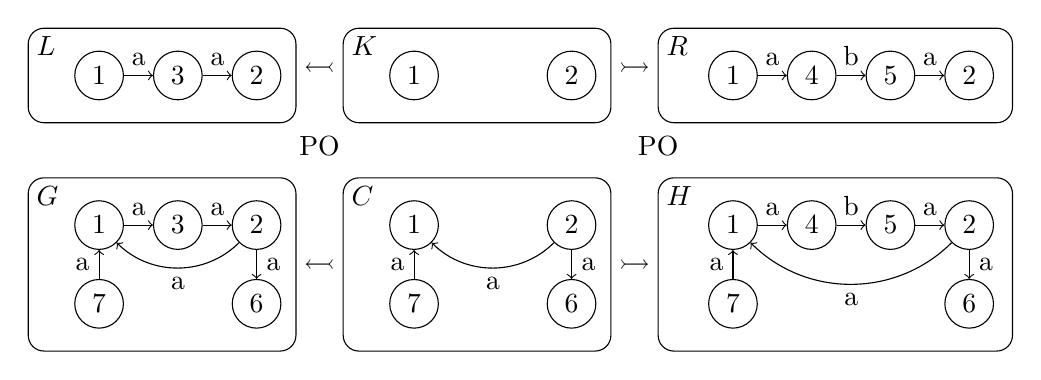
\begin{tikzpicture}
                \graphbox{\( L \)}{0mm}{-3mm}{34mm}{12mm}{2mm}{2mm}{
                    \coordinate (o) at (0mm,-8mm); 
                    \node[draw,circle] (l1) at ($(o)+(-10mm,0mm)$) {1};
                    \node[draw,circle] (l2) at ($(l1)+(2,0)$) {2};
                    \node[draw,circle] (l3) at ($(l1) + (1,0)$) {3};
                    \draw[->] (l1) -- (l3) node[midway,above] {a};
                    \draw[->] (l3) -- (l2) node[midway,above] {a};
                } 
        
                \graphbox{\( K \)}{40mm}{-3mm}{34mm}{12mm}{2mm}{2mm}{
                    \coordinate (o) at (0mm,-8mm); 
                    \node[draw,circle] (l1) at ($(o)+(-10mm,0mm)$) {1};
                    \node[draw,circle] (l2) at ($(l1)+(2,0)$) {2};
                }  
        
                \graphbox{\( R \)}{80mm}{-3mm}{45mm}{12mm}{2mm}{2mm}{
                    \coordinate (o) at (-5mm,-8mm); 
                    \node[draw,circle] (l1) at ($(o)+(-10mm,0mm)$) {1};
                    \node[draw,circle] (l2) at ($(l1)+(3,0)$) {2};
                    \node[draw,circle] (l3) at ($(l1) + (1,0)$) {4};
                    \node[draw,circle] (l4) at ($(l1) + (2,0)$) {5};
                    \draw[->] (l1) -- (l3) node[midway,above] {a};
                    \draw[->] (l3) -- (l4) node[midway,above] {b};
                    \draw[->] (l4) -- (l2) node[midway,above] {a};
                }    
        
                \graphbox{\( G \)}{0mm}{-22mm}{34mm}{22mm}{2mm}{-3mm}{
                    \coordinate (o) at (0mm,-3mm); 
                    \node[draw,circle] (l1) at ($(o)+(-10mm,0mm)$) {1};
                    \node[draw,circle] (l2) at ($(l1)+(2,0)$) {2};
                    \node[draw,circle] (l3) at ($(l1) + (1,0)$) {3};
                    \node[draw,circle] (l4) at ($(l2) + (0,-1)$) {6};
                    \draw[->] (l1) -- (l3) node[midway,above] {a};
                    \draw[->] (l3) -- (l2) node[midway,above] {a};
                    \draw[->] (l2) -- (l4) node[midway,right] {a};
                    \node[draw,circle] (l6) at ($(l1) + (0,-1)$) {7};
                    \draw[<-] (l1) -- (l6) node[midway,left] {a};
                    \draw[->] (l2) edge[out=-135,in=-45]node[midway,below] {a} (l1) ;
                }    
        
                \graphbox{\( C  \)}{40mm}{-22mm}{34mm}{22mm}{2mm}{-3mm}{
                    \coordinate (o) at (0mm,-3mm); 
                    \node[draw,circle] (l1) at ($(o)+(-10mm,0mm)$) {1};
                    \node[draw,circle] (l2) at ($(l1)+(2,0)$) {2};
                    \node[draw,circle] (l4) at ($(l2) + (0,-1)$) {6};
                    \draw[->] (l2) -- (l4) node[midway,right] {a};
                    \draw[->] (l2) edge[out=-135,in=-45]node[midway,below] {a} (l1) ;
                    \node[ draw,circle] (l6) at ($(l1) + (0,-1)$) {7};
                    \draw[<-] (l1) -- (l6) node[midway,left] {a};
                }    
        
                \graphbox{\( H \)}{80mm}{-22mm}{45mm}{22mm}{2mm}{-3mm}{
                    \coordinate (o) at (-5mm,-3mm); 
                    \node[draw,circle] (l1) at ($(o)+(-10mm,0mm)$) {1};
                    \node[draw,circle] (l2) at ($(l1)+(3,0)$) {2};
                    \node[draw,circle] (l3) at ($(l1) + (1,0)$) {4};
                    \node[draw,circle] (l4) at ($(l1) + (2,0)$) {5};
                    \node[ draw,circle] (l5) at ($(l2) + (0,-1)$) {6};
                    \node[ draw,circle] (l6) at ($(l1) + (0,-1)$) {7};
                    \draw[<-] (l1) -- (l6) node[midway,left] {a};
                    \draw[->] (l1) -- (l3) node[midway,above] {a};
                    \draw[->] (l3) -- (l4) node[midway,above] {b};
                    \draw[->] (l4) -- (l2) node[midway,above] {a};
                    \draw[->] (l2) -- (l5) node[midway,right] {a};
                    \draw[->] (l2) edge[out=-135,in=-45]node[midway,below] {a} (l1) ;
                }    
        
                \node () at (37mm,-8mm) {\( \leftarrowtail \)}; % K -> L
                \node () at (77mm,-8mm) {\( \rightarrowtail \)}; % K -> R
                \node () at (15mm,-18mm) {\(\downarrowtail \)};
                \node () at (37mm,-33mm) {\( \leftarrowtail \)};
                \node () at (37mm,-18mm) {PO};
                \node () at (58mm,-18mm) {\( \downarrowtail \)};
                \node () at (80mm,-18mm) {PO};
                \node () at (102mm,-18mm) {\( \downarrowtail \)};
                \node () at (77mm,-33mm) {\( \rightarrowtail \)}; % C -> H
            \end{tikzpicture}
            }         
        \end{center}

        An implicit occurrence of chain  \tikz[baseline=-0.5ex]{ 
        \node (x) at (0,0) {$\bullet$};  
        \node (y) at (1,0) {$\bullet$};
        \node (z) at (2,0) {$\bullet$};
        \draw[->] (x) -- node[midway,below] {a} (y) ;
        \draw[->] (y) -- node[midway,below] {a} (z) ;
        } in \(H\) and its coressponding implicit occurrence in \(G\):

         \begin{center} 
        \resizebox{0.9\textwidth}{!}{
        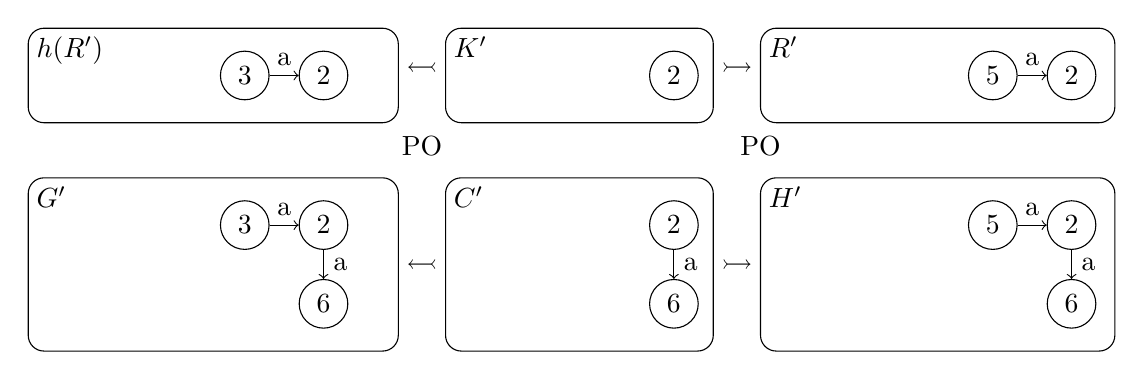
\begin{tikzpicture}
            \graphbox{\( h(R') \)}{-13mm}{-3mm}{47mm}{12mm}{2mm}{2mm}{
                \coordinate (o) at (2mm,-8mm); 
                \node[circle] (l1) at ($(o)+(-10mm,0mm)$) {};
                \node[draw,circle] (l2) at ($(l1)+(2,0)$) {2};
                \node[draw,circle] (l3) at ($(l1) + (1,0)$) {3};
                % \draw[->] (l1) -- (l3) node[midway,above] {a};
                \draw[->] (l3) -- (l2) node[midway,above] {a};
            } 
    
            \graphbox{\( R' \)}{80mm}{-3mm}{45mm}{12mm}{2mm}{2mm}{
                \coordinate (o) at (-5mm,-8mm); 
                \node[circle] (l1) at ($(o)+(-10mm,0mm)$) {};
                \node[draw,circle] (l2) at ($(l1)+(3,0)$) {2};
                % \node[draw,circle] (l3) at ($(l1) + (1,0)$) {4};
                \node[draw,circle] (l4) at ($(l1) + (2,0)$) {5};
                % \draw[->] (l1) -- (l3) node[midway,above] {a};
                % \draw[->] (l3) -- (l4) node[midway,above] {b};
                \draw[->] (l4) -- (l2) node[midway,above] {a};
            }    
    
            \graphbox{\( G'\)}{-13mm}{-22mm}{47mm}{22mm}{2mm}{-3mm}{
                \coordinate (o) at (2mm,-3mm); 
                \node[circle] (l1) at ($(o)+(-10mm,0mm)$) {};
                \node[draw,circle] (l2) at ($(l1)+(2,0)$) {2};
                \node[draw,circle] (l3) at ($(l1) + (1,0)$) {3};
                \node[draw,circle] (l4) at ($(l2) + (0,-1)$) {6};
                % \draw[->] (l1) -- (l3) node[midway,above] {a};
                \draw[->] (l3) -- (l2) node[midway,above] {a};
                \draw[->] (l2) -- (l4) node[midway,right] {a};
                % \node[draw,circle] (l6) at ($(l1) + (0,-1)$) {7};
                % \draw[<-] (l1) -- (l6) node[midway,left] {a};
                % \draw[->] (l2) edge[out=-135,in=-45]node[midway,below] {a} (l1) ;
            }    
    
            \graphbox{\( K' \)}{40mm}{-3mm}{34mm}{12mm}{2mm}{2mm}{
                \coordinate (o) at (0mm,-8mm); 
                \node[circle] (l1) at ($(o)+(-10mm,0mm)$) {};
                \node[draw,circle] (l2) at ($(l1)+(2,0)$) {2};
            } 
            \graphbox{\( C'  \)}{40mm}{-22mm}{34mm}{22mm}{2mm}{-3mm}{
                \coordinate (o) at (0mm,-3mm); 
                \node[circle] (l1) at ($(o)+(-10mm,0mm)$) {};
                \node[draw,circle] (l2) at ($(l1)+(2,0)$) {2};
                \node[draw,circle] (l4) at ($(l2) + (0,-1)$) {6};
                \draw[->] (l2) -- (l4) node[midway,right] {a};
                % \draw[->] (l2) edge[out=-135,in=-45]node[midway,below] {a} (l1) ;
                % \node[ draw,circle] (l6) at ($(l1) + (0,-1)$) {7};
                % \draw[<-] (l1) -- (l6) node[midway,left] {a};
            }  
    
            \graphbox{\( H' \)}{80mm}{-22mm}{45mm}{22mm}{2mm}{-3mm}{
                \coordinate (o) at (-5mm,-3mm); 
                \node[circle] (l1) at ($(o)+(-10mm,0mm)$) {};
                \node[draw,circle] (l2) at ($(l1)+(3,0)$) {2};
                \node[circle] (l3) at ($(l1) + (1,0)$) {};
                \node[draw,circle] (l4) at ($(l1) + (2,0)$) {5};
                \node[ draw,circle] (l5) at ($(l2) + (0,-1)$) {6};
                \node[circle] (l6) at ($(l1) + (0,-1)$) {};
                % \draw[<-] (l1) -- (l6) node[midway,left] {a};
                % \draw[->] (l1) -- (l3) node[midway,above] {a};
                % \draw[->] (l3) -- (l4) node[midway,above] {b};
                \draw[->] (l4) -- (l2) node[midway,above] {a};
                \draw[->] (l2) -- (l5) node[midway,right] {a};
                % \draw[->] (l2) edge[out=-135,in=-45]node[midway,below] {a} (l1) ;
            }    
            % \graphbox{$L$}{133mm}{-3mm}{34mm}{12mm}{2mm}{2mm}{
            %     \coordinate (o) at (0mm,-8mm); 
            %     \node[draw,circle] (l1) at ($(o)+(-10mm,0mm)$) {};
            %     \node[draw,circle] (l2) at ($(l1)+(2,0)$) {2};
            %     \node[draw,circle] (l3) at ($(l1) + (1,0)$) {5};
            %     \draw[->] (l1) -- (l3) node[midway,above] {a};
            %     \draw[->] (l3) -- (l2) node[midway,above] {a};
            % }
            % \node () at (129mm,-8mm) {\textcolor{red}{\( \rightarrowtail \)}};
            \node () at (37mm,-8mm) {\( \leftarrowtail \)}; % K -> L
            \node () at (77mm,-8mm) {\( \rightarrowtail \)}; % K -> R
            \node () at (15mm,-18mm) {\(\downarrowtail \)};
            \node () at (37mm,-33mm) {\( \leftarrowtail \)};
            \node () at (37mm,-18mm) {PO};
            \node () at (58mm,-18mm) {\( \downarrowtail \)};
            \node () at (80mm,-18mm) {PO};
            \node () at (102mm,-18mm) {\( \downarrowtail \)};
            \node () at (77mm,-33mm) {\( \rightarrowtail \)}; % C -> H
        \end{tikzpicture}
        }         
    \end{center}
\end{frame}

% \begin{frame}
%  \begin{center}
%        \resizebox{0.49\textwidth}{!}{
%         \begin{tikzpicture}
%             % [node distance=15mm]
%             \node (I) at (0,0) {$K$};
%             \node (L)  at (-2,0) {$L$};
%             \node (R)  at (2,0) {$R$};
%             \node (G)  at (-2,-2) {$G$};
%             \node (C)  at (0,-2) {$C$};
%             \node (H)  at (2,-2) {$H$};
%             \draw [>->] (I) to  node [midway,below] { } (L);
%             \draw [>->] (I) to  node [midway,below] { } (R);
%             \draw [>->] (L) to node [midway,right] { } (G);
%             \draw [>->] (I) to  node [midway,right] 
%             % {$u$}
%             {} (C);
%             \draw [>->] (R) to  node [midway,right] 
%             {$m'$}
%             (H);
%             \draw [>->] (C) to node [midway,above] {} (G);
%             \draw [>->] (C) to node [midway,above] 
%             {}
%             (H);
%             % \node [at=($(I)!.5!(G)$)] {\normalfont PO};
%             % \node [at=($(I)!.5!(H)$)] {\normalfont PO};
%         \end{tikzpicture}
%     }
%     \resizebox{0.49\textwidth}{!}{
%             \begin{tikzpicture} 
%                 \coordinate (k) at (0, 0);
%                 \draw[fill=white] ($(k)+(0,0)$) rectangle ($(k)+(0.5,0.5)$);
%                 \node () at ($(k)+(0.25,0.25)$) {\( \mathrm{K} \)};
            
%                 \coordinate (c) at (0, -2.2);
%                 \draw[fill=blue!20]
%                 ($(c)+(0,-0.5)$)
%                 -- ($(c)+(0,0.5)$) 
%                 -- ($(c)+(1,0.5)$) 
%                 arc[start angle=0, end angle=-90, radius=1]
%                 -- cycle;
%                 \node () at ($(c)+(0.75,0.25)$) {\( \mathrm{C'} \)};
%                 \draw[fill=white] ($(c)+(0,0)$) rectangle ($(c)+(0.5,0.5)$);
%                 \node () at ($(c)+(0.25,0.25)$) {\( \mathrm{K} \)};
            
%                 \coordinate (l) at (-3, 0);
%                 \draw[fill=orange!20] ($(l)+(-0.5,0)$) rectangle ($(l)+(0.5,1)$);
%                 \node () at ($(l)+(-0.23,0.25)$) {\( \mathrm{L'} \)};
%                 \draw[fill=white] ($(l)+(0,0)$) rectangle ($(l)+(0.5,0.5)$);
%                 \node () at ($(l)+(0.25,0.25)$) {\( \mathrm{K} \)};
            
%                 \coordinate (g) at (-3, -2.2);
%                 \draw[fill=blue!20]
%                 ($(g)+(0,-0.5)$)
%                 -- ($(g)+(0,0.5)$)
%                 -- ($(g)+(1,0.5)$) 
%                 arc[start angle=0, end angle=-90, radius=1]
%                 -- cycle;
%                 \draw[fill=orange!20] ($(g)+(-0.5,0)$) rectangle ($(g)+(0.5,1)$);
%                 \node () at ($(g)+(0.75,0.25)$) {\( \mathrm{C'} \)};
%                 \node () at ($(g)+(-0.23,0.25)$) {\( \mathrm{L'} \)};
%                 \draw[fill=white] ($(g)+(0,0)$) rectangle ($(g)+(0.5,0.5)$);
%                 \node () at ($(g)+(0.25,0.25)$) {\( \mathrm{K} \)};
            
%                 \coordinate (r) at (3,0);
%                 \draw[fill=red!20] ($(r)+(-0.5,0)$)
%                 -- ($(r)+(-0.5,0.5)$)
%                 -- ($(r)+(0,1)$)
%                 --  ($(r)+(0.5,1)$)
%                 -- ($(r)+(0.5,0)$)
%                 -- cycle;
%                 \node () at ($(r)+(-0.23,0.25)$) {\( \mathrm{R'} \)};
%                 \draw[fill=white] ($(r)+(0,0)$) rectangle ($(r)+(0.5,0.5)$);
%                 \node () at ($(r)+(0.25,0.25)$) {\( \mathrm{K} \)};
            
%                 \coordinate (h) at (3, -2.2);
%                 \draw[fill=blue!20]
%                 ($(h)+(0,-0.5)$)
%                 -- ($(h)+(0,0.5)$)
%                 -- ($(h)+(1,0.5)$) 
%                 arc[start angle=0, end angle=-90, radius=1]
%                 -- cycle;
%                 \draw[fill=red!20] ($(h)+(-0.5,0)$)
%                 -- ($(h)+(-0.5,0.5)$)
%                 -- ($(h)+(0,1)$)
%                 --  ($(h)+(0.5,1)$)
%                 -- ($(h)+(0.5,0)$)
%                 -- cycle;
%             \node () at ($(h)+(0.75,0.25)$) {\( \mathrm{C'} \)};
%             \draw[fill=white] ($(h)+(0,0)$) rectangle ($(h)+(0.5,0.5)$);
%             \node () at ($(h)+(0.25,0.25)$) {\( \mathrm{K} \)};
%             \node () at ($(h)+(-0.23,0.25)$) {\( \mathrm{R'} \)};
            
%                 \node[ font=\huge] (kl) at ($(k)!0.5!(l)+(0.25,0.25)$)
%             %    {\( \overset{l}{\leftarrowtail} \)}
%                 {\( \leftarrowtail \)}
%                 ; 
%                 \node[ font=\huge] (kr) at ($(k)!0.5!(r)+(0.25,0.25)$)
%                 {\( \rightarrowtail \)}
%                 ;  
%                 \node[ font=\huge] (cg) at ($(c)!0.5!(g)+(0.25,0.25)$) 
%                 {\( \leftarrowtail \)}
%             ;  
%                 \node[ font=\huge] (ch) at ($(c)!0.5!(h)+(0.25,0.25)$)
%                 {\( \rightarrowtail \)}
%             ; 
%                 \node[ font=\huge] (kc) at ($(k)!0.5!(c)+(0.2,0.4)$) {\( \downarrowtail \)}; 
%             %   \node[ font=\LARGE] () at ($(l)!0.5!(g)+(0.5,0.4)$) {$m$}; 
%                 \node[ font=\huge] (lg) at ($(l)!0.5!(g)+(0.1,0.4)$) {\( \downarrowtail \)}; 
%                 \node[ font=\huge] (rh) at ($(r)!0.5!(h)+(0.1,0.4)$) {\( \downarrowtail \)}; 
%             %   \node[ font=\LARGE] () at ($(r)!0.5!(h)+(0.55,0.4)$) {$m'$}; 
%             %   \node[ font=\LARGE] () at ($(k)!0.5!(c)+(0.5,0.4)$) {$u$}; 
%             \end{tikzpicture}
%           }
%    \end{center}

%    Implicit $X$-occurrence $x$ in $G$ is of form $L_x \cup C'_x$ 
     
%    Implicit $X$-occurrence $x$ in $G$ is of form $R_x \cup C'_x$
    
%     It suffices to map different $R_x$ to different $L_x$ in such a way that 
%     \begin{itemize}
%         \item there is an injection from implicit $X$-occurrences in $H$ to implicit $X$-occurrences in $G$ 
%     \end{itemize}
% \end{frame}


% \begin{frame}{The set $D(R,X)$ of all subgraphs of $R$ that can form an implicitly created $X$-occurrence in some rewriting step}
%     % $D(L,X)$ : set of all subgraphs of $L$ that can form an implicitly deleted $X$-occurrence in some rewriting step
%     Example:
%      \begin{center}
%         \resizebox{\textwidth}{!}{ 
%             \begin{tikzpicture}
%                 \graphbox{$L$}{0mm}{0mm}{35mm}{35mm}{2mm}{-5mm}{
%                     \coordinate (delta) at (0,-18mm);
%                     \node[draw,circle] (l1) at ($(delta) + (-1,1.5)$) {1};
%                     \node[draw,circle] (l2) at ($(delta) + (1,1.5)$) {2};
%                     \node[draw,circle] (l3) at ($(delta) + (0,0)$) {3};
%                     \draw[->] (l1) -- (l3) node[midway,left] {s};
%                     \draw[->] (l2) -- (l3) node[midway,right] {s};
%                     \draw[->] (l3) edge [loop below] node {0} (l3);
%                 }
%                     \graphbox{$K$}{40mm}{0mm}{35mm}{35mm}{2mm}{-5mm}{
%                         \coordinate (delta) at (0,-18mm);
%                         \coordinate (interfaceorigin) at ($(delta) +(5,0)$);
%                         \node[draw,circle] (r1) at ($(delta) +(-1,1.5)$) {1};
%                         \node[draw,circle] (r2) at ($(delta) +(0.5,1.5)$) {2};
%                         \node[draw,circle] (r3) at ($(delta) + (0,0)$) {3};
%                         % \draw[->] (r1) -- (r3) node[midway,left] {s};
%                         % \draw[->] (r3) edge [loop below] node {0} (r3);
%                     } 
%                     \node () at (38mm,-18mm) {$\leftarrowtail$};
%                     \node () at (77mm,-18mm) {$\rightarrowtail$};
%                 \graphbox{$R$}{80mm}{0mm}{50mm}{35mm}{2mm}{-5mm}{
%                     \coordinate (delta) at (-10mm,-18mm);
%                     \node[draw,circle] (r1) at ($(delta) + (-1,1.5)$) {1};
%                     \node[draw,circle] (r2) at ($(delta) + (0.5,1.5)$) {2};
%                     \node[draw,circle] (r3) at ($(delta) + (0,0)$) {3};
%                     \node[draw,circle] (r4) at ($(delta) + (1,0)$) {};
%                     \draw[->] (r1) -- (r3) node[midway,left] {s};
%                     \draw[->] (r2) -- (r4) node[midway,right] {s};
%                     \draw[->] (r4) edge [loop below] node {0} (r4);
%                     \draw[->] (r3) edge [loop below] node {0} (r3);
%                     \node[draw,circle] (r5) at ($(r2) + (1.5,0)$) {};
%                     \draw[->] (r5) edge [loop below] node {0} (r5);
%                     \draw[->] (r5) edge [loop right] node {0} (r5);
%                     \draw[->] (r5) edge [loop left] node {0} (r5);
%                 }
%                 % \graphbox{$R_x$}{40mm}{40mm}{35mm}{35mm}{2mm}{-5mm}{
%                 %     \coordinate (delta) at (0,-18mm);
%                 %     \coordinate (rxorigin) at ($(interfaceorigin)+(0,6)$);
%                 %     \node[draw,circle] (r1) at ($(delta) + (-1,1.5)$) {1};
%                 %     \node[draw,circle] (r2) at ($(delta) +  (0.5,1.5)$) {2};
%                 %     \node[draw,circle] (r3) at ($(delta) +  (0,0)$) {3};
%                 %     \draw[->] (r1) -- (r3) node[midway,left] {s};
%                 %     % \draw[->] (r3) edge [loop below] node {0} (r3);
%                 % }
                
%                 % \node () at (57mm,2mm) {$\uparrowtail$};
%                 % \node () at (38mm,2mm) {$\swarrowtail$};
%                 % \node () at (79mm,2mm) {$\searrowtail$};
%             \end{tikzpicture}
%             }
%     \end{center}

%     $X$ : the graph $\tikz[baseline=-0.5ex]{ 
%                 \node (x) at (0,0) {$\bullet$}; 
%                 \node (y) at (1,0) {$\bullet$};
%                 \node (z) at (2,0) {$\bullet$};
%                 \draw[->] (x) -- (y) node[midway, above] {$s$};
%                 \draw[->] (z) -- (y) node[midway, above] {$s$};
%         }$

%     % $D(L,X)$: $L'_1$:
%     %     \raisebox{2pt}{
%     %         \scalebox{0.7}{\tikz[baseline=-0.5ex]{
%     %         \node [draw,circle] (x) at (0,0) {1};
%     %         \node[draw,circle] (y) at (1,0) {3};
%     %         \draw[->] (x) -- (y) node[midway, above] {$s$};
%     %     }}}, $L'_2$:
%     %     \raisebox{2pt}{
%     %         \scalebox{0.7}{\tikz[baseline=-0.5ex]{
%     %         \node [draw,circle] (z) at (2,0) {2};
%     %         \node [draw,circle] (x) at (0,0) {1};
%     %         \node[draw,circle] (y) at (1,0) {3};
%     %         \draw[->] (x) -- (y) node[midway, above] {$s$};
%     %     }}}, 
%     %     $L'_3$:
%     %     \raisebox{2pt}{
%     %         \scalebox{0.7}{\tikz[baseline=-0.5ex]{
%     %         \node [draw,circle] (z) at (2,0) {2};
%     %         \node [draw,circle] (y) at (1,0) {3};
%     %         \draw[->] (z) -- (y) node[midway, above] {$s$};
%     %     }}},
%     %     $L'_4$:
%     %     \raisebox{2pt}{
%     %         \scalebox{0.7}{\tikz[baseline=-0.5ex]{
%     %         \node [draw,circle] (z) at (2,0) {2};
%     %         \node [draw,circle] (x) at (0,0) {1};
%     %         \node[draw,circle] (y) at (1,0) {3};
%     %         \draw[->] (z) -- (y) node[midway, above] {$s$};
%     %     }}}

%     $D(R,X)$ consists of $R_1$:
%         \raisebox{2pt}{
%             \scalebox{0.7}{\tikz[baseline=-0.5ex]{
%             \node [draw,circle] (x) at (0,0) {1};
%             \node[draw,circle] (y) at (1,0) {3};
%             \draw[->] (x) -- (y) node[midway, above] {$s$};
%         }}} and $R_2$:
%         \raisebox{2pt}{
%             \scalebox{0.7}{\tikz[baseline=-0.5ex]{
%             \node [draw,circle] (z) at (2,0) {2};
%             \node [draw,circle] (x) at (0,0) {1};
%             \node[draw,circle] (y) at (1,0) {3};
%             \draw[->] (x) -- (y) node[midway, above] {$s$};
%         }}}
% \end{frame}

\begin{frame}{Distinguished Subgraph $D(R,X)$ : subgraphs of $R$ which can form an implicit $X$-occurrence in some rewriting step}
    Running example:
     \begin{center} 
            \resizebox{\textwidth}{!}{
           \begin{tikzpicture}
                \graphbox{\( L \)}{0mm}{-3mm}{34mm}{12mm}{2mm}{2mm}{
                    \coordinate (o) at (0mm,-8mm); 
                    \node[draw,circle] (l1) at ($(o)+(-10mm,0mm)$) {1};
                    \node[draw,circle] (l2) at ($(l1)+(2,0)$) {2};
                    \node[draw,circle] (l3) at ($(l1) + (1,0)$) {};
                    \draw[->] (l1) -- (l3) node[midway,above] {a};
                    \draw[->] (l3) -- (l2) node[midway,above] {a};
                } 
        
                \graphbox{\( K \)}{40mm}{-3mm}{34mm}{12mm}{2mm}{2mm}{
                    \coordinate (o) at (0mm,-8mm); 
                    \node[draw,circle] (l1) at ($(o)+(-10mm,0mm)$) {1};
                    \node[draw,circle] (l2) at ($(l1)+(2,0)$) {2};
                }  
        
                \graphbox{\( R \)}{80mm}{-3mm}{45mm}{12mm}{2mm}{2mm}{
                    \coordinate (o) at (-5mm,-8mm); 
                    \node[draw,circle] (l1) at ($(o)+(-10mm,0mm)$) {1};
                    \node[draw,circle] (l2) at ($(l1)+(3,0)$) {2};
                    \node[draw,circle] (l3) at ($(l1) + (1,0)$) {};
                    \node[draw,circle] (l4) at ($(l1) + (2,0)$) {};
                    \draw[->] (l1) -- (l3) node[midway,above] {a};
                    \draw[->] (l3) -- (l4) node[midway,above] {b};
                    \draw[->] (l4) -- (l2) node[midway,above] {a};
                }    
                \node () at (37mm,-8mm) {\( \overset{l}{\leftarrowtail} \)}; % K -> L
                \node () at (77mm,-8mm) {\( \overset{r}{\rightarrowtail} \)}; % K -> R
            \end{tikzpicture}
            }         
        \end{center}
    $D(R,X)$ consists of :
\begin{center}
        \resizebox{0.45\textwidth}{!}{
            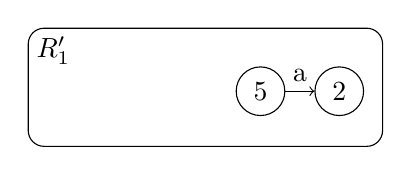
\begin{tikzpicture}
                \graphbox{$R'_1$}{70mm}{0mm}{45mm}{15mm}{2mm}{-5mm}{
                    \coordinate (o) at (-5mm,-3mm); 
                    \node[circle] (l1) at ($(o)+(-10mm,0mm)$) {};
                    \node[draw,circle] (l2) at ($(l1)+(3,0)$) {2};
                    \node[draw,circle] (l4) at ($(l1) + (2,0)$) {5};
                    \draw[->] (l4) -- (l2) node[midway,above] {a};
                }    
            \end{tikzpicture}
        }
    %     \end{center}
    % \begin{center}
        \resizebox{0.45\textwidth}{!}{
            \begin{tikzpicture}
                \graphbox{$R'_2$}{70mm}{0mm}{45mm}{15mm}{2mm}{-5mm}{
                    \coordinate (o) at (-5mm,-3mm); 
                    \node[draw,circle] (l1) at ($(o)+(-10mm,0mm)$) {1};
                    \node[draw,circle] (l2) at ($(l1)+(3,0)$) {2};
                    \node[draw,circle] (l4) at ($(l1) + (2,0)$) {5};
                    \draw[->] (l4) -- (l2) node[midway,above] {a};
                }    
            \end{tikzpicture}
        } 
        \end{center}
    \begin{center}
        \resizebox{0.45\textwidth}{!}{
            \begin{tikzpicture}
                \graphbox{$R'_3$}{70mm}{0mm}{45mm}{15mm}{2mm}{-5mm}{
                    \coordinate (o) at (-5mm,-3mm); 
                    \node[draw,circle] (l1) at ($(o)+(-10mm,0mm)$) {1};
                    \node[draw,circle] (l3) at ($(l1) + (1,0)$) {4};
                    \draw[->] (l1) -- (l3) node[midway,above] {a};
                }   
        \end{tikzpicture}
        } 
    %             \end{center}
    % \begin{center}
        \resizebox{0.45\textwidth}{!}{
            \begin{tikzpicture}
                \graphbox{$R'_4$}{70mm}{0mm}{45mm}{15mm}{2mm}{-5mm}{
                    \coordinate (o) at (-5mm,-3mm); 
                    \node[draw,circle] (l1) at ($(o)+(-10mm,0mm)$) {1};
                    \node[draw,circle] (l2) at ($(l1)+(3,0)$) {2};
                    \node[draw,circle] (l3) at ($(l1) + (1,0)$) {4};
                    \draw[->] (l1) -- (l3) node[midway,above] {a};
                }    
            \end{tikzpicture}
        }
    \end{center}
    
\end{frame}


\begin{frame}{Observation:For every $R_i \in D(R,X)$, there is a morphism \(h_i: R_i \rightarrowtail L \) which preserves the interface elements}
    
    \begin{center}  
        \resizebox{\textwidth}{!}{
        \begin{tikzpicture}    
            \graphbox{\( K'_1 \)}{40mm}{-3mm}{34mm}{12mm}{2mm}{2mm}{
                \coordinate (o) at (0mm,-8mm); 
                \node[circle] (l1) at ($(o)+(-10mm,0mm)$) {};
                \node[draw,circle] (l2) at ($(l1)+(2,0)$) {2};
            } 
            \graphbox{\( R'_1 \)}{80mm}{-3mm}{45mm}{12mm}{2mm}{2mm}{
                \coordinate (o) at (-5mm,-8mm); 
                \node[circle] (l1) at ($(o)+(-10mm,0mm)$) {};
                \node[draw,circle] (l2) at ($(l1)+(3,0)$) {2};
                \node[draw,circle] (l4) at ($(l1) + (2,0)$) {5};
                \draw[->] (l4) -- (l2) node[midway,above] {a};
            } 
            \graphbox{$L$}{133mm}{-3mm}{34mm}{12mm}{2mm}{2mm}{
                \coordinate (o) at (0mm,-8mm); 
                \node[draw,circle] (l1) at ($(o)+(-10mm,0mm)$) {};
                \node[draw,circle] (l2) at ($(l1)+(2,0)$) {2};
                \node[draw,circle] (l3) at ($(l1) + (1,0)$) {5};
                \draw[->] (l1) -- (l3) node[midway,above] {a};
                \draw[->] (l3) -- (l2) node[midway,above] {a};
            }
            \node () at (129mm,-8mm) {\(\overset{\textcolor{red}{h_1}}{\rightarrowtail}\)};
            \node () at (77mm,-8mm) {\( \rightarrowtail \)}; % K -> R
        \end{tikzpicture}
        }         
    \end{center}

    \begin{center} 
        \resizebox{\textwidth}{!}{
        \begin{tikzpicture}
            \graphbox{\( K'_2  \)}{40mm}{-3mm}{34mm}{12mm}{2mm}{2mm}{
                \coordinate (o) at (0mm,-8mm); 
                \node[draw,circle] (l1) at ($(o)+(-10mm,0mm)$) {1};
                \node[draw,circle] (l2) at ($(l1)+(2,0)$) {2};
            }  
    
            \graphbox{\( R_2' \)}{80mm}{-3mm}{45mm}{12mm}{2mm}{2mm}{
                \coordinate (o) at (-5mm,-8mm); 
                \node[draw,circle] (l1) at ($(o)+(-10mm,0mm)$) {1};
                \node[draw,circle] (l2) at ($(l1)+(3,0)$) {2};
                \node[draw,circle] (l4) at ($(l1) + (2,0)$) {5};
                \draw[->] (l4) -- (l2) node[midway,above] {a};
            }     
     
            \graphbox{$L$}{133mm}{-3mm}{34mm}{12mm}{2mm}{2mm}{
                \coordinate (o) at (0mm,-8mm); 
                \node[draw,circle] (l1) at ($(o)+(-10mm,0mm)$) {1};
                \node[draw,circle] (l2) at ($(l1)+(2,0)$) {2};
                \node[draw,circle] (l3) at ($(l1) + (1,0)$) {5};
                \draw[->] (l1) -- (l3) node[midway,above] {a};
                \draw[->] (l3) -- (l2) node[midway,above] {a};
            }
            \node () at (129mm,-8mm) {\(\overset{\textcolor{red}{h_2}}{\rightarrowtail}\)};
            \node () at (77mm,-8mm) {\( \rightarrowtail \)}; % K -> R
        \end{tikzpicture}
        }         
    \end{center}

    \begin{center} 
        \resizebox{\textwidth}{!}{
        \begin{tikzpicture}
            \graphbox{\( K'_3 \)}{40mm}{-3mm}{34mm}{12mm}{2mm}{2mm}{
                \coordinate (o) at (0mm,-8mm); 
                \node[draw,circle] (l1) at ($(o)+(-10mm,0mm)$) {1};
            }  
    
            \graphbox{\( R'_3 \)}{80mm}{-3mm}{45mm}{12mm}{2mm}{2mm}{
                \coordinate (o) at (-5mm,-8mm); 
                \node[draw,circle] (l1) at ($(o)+(-10mm,0mm)$) {1};
                \node[draw,circle] (l3) at ($(l1) + (1,0)$) {4};
                \draw[->] (l1) -- (l3) node[midway,above] {a};
            }    
            \graphbox{$L$}{133mm}{-3mm}{34mm}{12mm}{2mm}{2mm}{
                \coordinate (o) at (0mm,-8mm); 
                \node[draw,circle] (l1) at ($(o)+(-10mm,0mm)$) {1};
                \node[draw,circle] (l2) at ($(l1)+(2,0)$) {};
                \node[draw,circle] (l3) at ($(l1) + (1,0)$) {4};
                \draw[->] (l1) -- (l3) node[midway,above] {a};
                \draw[->] (l3) -- (l2) node[midway,above] {a};
            }
            \node () at (129mm,-8mm) {\(\overset{\textcolor{red}{h_3}}{\rightarrowtail}\)};
            \node () at (77mm,-8mm) {\( \rightarrowtail \)}; % K -> R
        \end{tikzpicture}
        }         
    \end{center}

       \begin{center} 
        \resizebox{\textwidth}{!}{
        \begin{tikzpicture}
            \graphbox{\( K'_4 \)}{40mm}{-3mm}{34mm}{12mm}{2mm}{2mm}{
                \coordinate (o) at (0mm,-8mm); 
                \node[draw,circle] (l1) at ($(o)+(-10mm,0mm)$) {1};
                \node[draw,circle] (l2) at ($(l1)+(2,0)$) {2};

            }  
    
            \graphbox{\( R'_4 \)}{80mm}{-3mm}{45mm}{12mm}{2mm}{2mm}{
                \coordinate (o) at (-5mm,-8mm); 
                \node[draw,circle] (l1) at ($(o)+(-10mm,0mm)$) {1};
                \node[draw,circle] (l2) at ($(l1)+(3,0)$) {2};
                \node[draw,circle] (l3) at ($(l1) + (1,0)$) {4};
                % \node[draw,circle] (l4) at ($(l1) + (2,0)$) {5};
                \draw[->] (l1) -- (l3) node[midway,above] {a};
                % \draw[->] (l3) -- (l4) node[midway,above] {b};
                % \draw[->] (l4) -- (l2) node[midway,above] {a};
            }    
            \graphbox{$L$}{133mm}{-3mm}{34mm}{12mm}{2mm}{2mm}{
                \coordinate (o) at (0mm,-8mm); 
                \node[draw,circle] (l1) at ($(o)+(-10mm,0mm)$) {1};
                \node[draw,circle] (l2) at ($(l1)+(2,0)$) {2};
                \node[draw,circle] (l3) at ($(l1) + (1,0)$) {4};
                \draw[->] (l1) -- (l3) node[midway,above] {a};
                \draw[->] (l3) -- (l2) node[midway,above] {a};
            }
            \node () at (129mm,-8mm) {\(\overset{\textcolor{red}{h_4}}{\rightarrowtail}\)};
            \node () at (77mm,-8mm) {\( \rightarrowtail \)}; % K -> R
        \end{tikzpicture}
        }         
    \end{center}
\end{frame}

\begin{frame}{$X$-non-increasing rule}
 \begin{definition}
    A rule $\varphi$ is $X$-non-increasing rule if 
    \begin{enumerate}
        \item For every $R_i \in D(R,X)$, there is a morphism \(h_i: R_i \rightarrowtail L \) which preserves the interface elements,
        % \item For all $R'_i \in D(R,X)$, morphism $h_i$ does not maps any non-interface element to an interface element,
        % \item Different edges $e_i \in R_i$ and $e_j \in R_j$ have different images $h_{R_iL}(e_i) \neq h_{R_jL}(e_j)$,
        % \item If $X$ has isolated nodes, then then for all $R',R'' \in D(R,X)$ and nodes $x \in R', y \in R''$, if $x \neq y$, then $h_{R'L}(x) \neq h_{R''L}(y)$.
        \item three more conditions on $h_i$
    \end{enumerate}  
 \end{definition}

    \begin{description}
    \item[Condition 1] guarantees every implicit $X$-occurrence in $H$ has a corresponding implicit $X$-occurrence in $G$ with the same interface elements

        \item[Other conditions] guarantee: different implicit $X$-occurrences in $H$ have different corresponding implicit $X$-occurrences in $G$
\end{description} 
\end{frame}

\begin{frame}{Main Results}
    Let $\varphi$ be a $X$-non-increasing rule.
    \begin{lemma}[More $X$-occurrences before rewriting]
        % If a rule $\varphi$ is $X$-non-increasing, then, 
        For all $G \Rightarrow_\varphi H$, there are more implicit $X$-occurrences in $G$ than in $H$.
    \end{lemma}
         
    \begin{theorem}[Sufficient Termination Condition]
        % If a rule $\varphi$ is $X$-non-increasing, then 
        $\varphi$ is terminating if there are strictly more explicit $X$-occurrences in $L$ than in $R$.
    \end{theorem}

\end{frame}


\begin{frame}{Terminating of Running Example}
     \begin{center} 
            \resizebox{\textwidth}{!}{
           \begin{tikzpicture}
                \graphbox{\( L \)}{0mm}{-3mm}{34mm}{12mm}{2mm}{2mm}{
                    \coordinate (o) at (0mm,-8mm); 
                    \node[draw,circle] (l1) at ($(o)+(-10mm,0mm)$) {1};
                    \node[draw,circle] (l2) at ($(l1)+(2,0)$) {2};
                    \node[draw,circle] (l3) at ($(l1) + (1,0)$) {};
                    \draw[->] (l1) -- (l3) node[midway,above] {a};
                    \draw[->] (l3) -- (l2) node[midway,above] {a};
                } 
        
                \graphbox{\( K \)}{40mm}{-3mm}{34mm}{12mm}{2mm}{2mm}{
                    \coordinate (o) at (0mm,-8mm); 
                    \node[draw,circle] (l1) at ($(o)+(-10mm,0mm)$) {1};
                    \node[draw,circle] (l2) at ($(l1)+(2,0)$) {2};
                }  
        
                \graphbox{\( R \)}{80mm}{-3mm}{45mm}{12mm}{2mm}{2mm}{
                    \coordinate (o) at (-5mm,-8mm); 
                    \node[draw,circle] (l1) at ($(o)+(-10mm,0mm)$) {1};
                    \node[draw,circle] (l2) at ($(l1)+(3,0)$) {2};
                    \node[draw,circle] (l3) at ($(l1) + (1,0)$) {};
                    \node[draw,circle] (l4) at ($(l1) + (2,0)$) {};
                    \draw[->] (l1) -- (l3) node[midway,above] {a};
                    \draw[->] (l3) -- (l4) node[midway,above] {b};
                    \draw[->] (l4) -- (l2) node[midway,above] {a};
                }    
                \node () at (37mm,-8mm) {\( \overset{l}{\leftarrowtail} \)}; % K -> L
                \node () at (77mm,-8mm) {\( \overset{r}{\rightarrowtail} \)}; % K -> R
            \end{tikzpicture}
            }         
    \end{center}
    \begin{itemize}
        \item X :  \tikz[baseline=-0.5ex]{ 
        \node (x) at (0,0) {$\bullet$};  
        \node (y) at (1,0) {$\bullet$};
        \node (z) at (2,0) {$\bullet$};
        \draw[->] (x) -- node[midway,below] {a} (y) ;
        \draw[->] (y) -- node[midway,below] {a} (z) ;
        }
        \item $X$-non-increasing rule
        \item Strictly more explicit $X$-occurrences in $L$ than in $R$: $1 \mathop{>} 0$.
    \end{itemize}
\end{frame}

\begin{frame}{Termination of Motivating Rule}
     \begin{center}
        \resizebox{\textwidth}{!}{ 
            \begin{tikzpicture}
                \graphbox{$L$}{0mm}{0mm}{35mm}{35mm}{2mm}{-5mm}{
                    \coordinate (delta) at (0,-18mm);
                    \node[draw,circle] (l1) at ($(delta) + (-1,1.5)$) {1};
                    \node[draw,circle] (l2) at ($(delta) + (1,1.5)$) {2};
                    \node[draw,circle] (l3) at ($(delta) + (0,0)$) {3};
                    \draw[->] (l1) -- (l3) node[midway,left] {s};
                    \draw[->] (l2) -- (l3) node[midway,right] {s};
                    \draw[->] (l3) edge [loop below] node {0} (l3);
                }
                    \graphbox{$K$}{40mm}{0mm}{35mm}{35mm}{2mm}{-5mm}{
                        \coordinate (delta) at (0,-18mm);
                        \coordinate (interfaceorigin) at ($(delta) +(5,0)$);
                        \node[draw,circle] (r1) at ($(delta) +(-1,1.5)$) {1};
                        \node[draw,circle] (r2) at ($(delta) +(0.5,1.5)$) {2};
                        \node[draw,circle] (r3) at ($(delta) + (0,0)$) {3};
                        % \draw[->] (r1) -- (r3) node[midway,left] {s};
                        % \draw[->] (r3) edge [loop below] node {0} (r3);
                    } 
                    \node () at (38mm,-18mm) {$\leftarrowtail$};
                    \node () at (77mm,-18mm) {$\rightarrowtail$};
                \graphbox{$R$}{80mm}{0mm}{50mm}{35mm}{2mm}{-5mm}{
                    \coordinate (delta) at (-10mm,-18mm);
                    \node[draw,circle] (r1) at ($(delta) + (-1,1.5)$) {1};
                    \node[draw,circle] (r2) at ($(delta) + (0.5,1.5)$) {2};
                    \node[draw,circle] (r3) at ($(delta) + (0,0)$) {3};
                    \node[draw,circle] (r4) at ($(delta) + (1,0)$) {};
                    \draw[->] (r1) edge[bend right] node[midway,left] {s} (r3) ;
                    \draw[->] (r2) -- (r4) node[midway,right] {s};
                    \draw[->] (r4) edge [loop below] node {0} (r4);
                    
                    \draw[->] (r3) edge [out=190,in=270,looseness=3] node[midway,left] {0} (r3);
                    \node[draw,circle] (r5) at ($(r2) + (1.5,0)$) {};
                    \draw[->] (r5) edge [loop below] node {0} (r5);
                    \draw[->] (r5) edge [loop right] node {0} (r5);
                    \draw[->] (r5) edge [loop left] node {0} (r5);
                }
                % \graphbox{$R_x$}{40mm}{40mm}{35mm}{35mm}{2mm}{-5mm}{
                %     \coordinate (delta) at (0,-18mm);
                %     \coordinate (rxorigin) at ($(interfaceorigin)+(0,6)$);
                %     \node[draw,circle] (r1) at ($(delta) + (-1,1.5)$) {1};
                %     \node[draw,circle] (r2) at ($(delta) +  (0.5,1.5)$) {2};
                %     \node[draw,circle] (r3) at ($(delta) +  (0,0)$) {3};
                %     \draw[->] (r1) -- (r3) node[midway,left] {s};
                %     % \draw[->] (r3) edge [loop below] node {0} (r3);
                % }
                
                % \node () at (57mm,2mm) {$\uparrowtail$};
                % \node () at (38mm,2mm) {$\swarrowtail$};
                % \node () at (79mm,2mm) {$\searrowtail$};
            \end{tikzpicture}
            }
    \end{center}

   

    % $D(L,X)$: $L'_1$:
    %     \raisebox{2pt}{
    %         \scalebox{0.7}{\tikz[baseline=-0.5ex]{
    %         \node [draw,circle] (x) at (0,0) {1};
    %         \node[draw,circle] (y) at (1,0) {3};
    %         \draw[->] (x) -- (y) node[midway, above] {$s$};
    %     }}}, $L'_2$:
    %     \raisebox{2pt}{
    %         \scalebox{0.7}{\tikz[baseline=-0.5ex]{
    %         \node [draw,circle] (z) at (2,0) {2};
    %         \node [draw,circle] (x) at (0,0) {1};
    %         \node[draw,circle] (y) at (1,0) {3};
    %         \draw[->] (x) -- (y) node[midway, above] {$s$};
    %     }}}, 
    %     $L'_3$:
    %     \raisebox{2pt}{
    %         \scalebox{0.7}{\tikz[baseline=-0.5ex]{
    %         \node [draw,circle] (z) at (2,0) {2};
    %         \node [draw,circle] (y) at (1,0) {3};
    %         \draw[->] (z) -- (y) node[midway, above] {$s$};
    %     }}},
    %     $L'_4$:
    %     \raisebox{2pt}{
    %         \scalebox{0.7}{\tikz[baseline=-0.5ex]{
    %         \node [draw,circle] (z) at (2,0) {2};
    %         \node [draw,circle] (x) at (0,0) {1};
    %         \node[draw,circle] (y) at (1,0) {3};
    %         \draw[->] (z) -- (y) node[midway, above] {$s$};
    %     }}}


    \begin{itemize}
        \item  $X$ : $\tikz[baseline=-0.5ex]{ 
                \node (x) at (0,0) {$\bullet$}; 
                \node (y) at (1,0) {$\bullet$};
                \node (z) at (2,0) {$\bullet$};
                \draw[->] (x) -- (y) node[midway, above] {$s$};
                \draw[->] (z) -- (y) node[midway, above] {$s$};
        }$
        \item $D(R,X)$ consists of $R_1$:
        \raisebox{2pt}{
            \scalebox{0.7}{\tikz[baseline=-0.5ex]{
            \node [draw,circle] (x) at (0,0) {1};
            \node[draw,circle] (y) at (1,0) {3};
            \draw[->] (x) -- (y) node[midway, above] {$s$};
        }}} and $R_2$:
        \raisebox{2pt}{
            \scalebox{0.7}{\tikz[baseline=-0.5ex]{
            \node [draw,circle] (z) at (2,0) {2};
            \node [draw,circle] (x) at (0,0) {1};
            \node[draw,circle] (y) at (1,0) {3};
            \draw[->] (x) -- (y) node[midway, above] {$s$};
        }}}
        \item $X$-non-increasing rule because inclusions from $h_1: R_1 \rightarrowtail L$ and $h_2: R_2 \rightarrowtail L$ satisfy all conditions.
        \item Strictly more explicit $X$-occurrences in $L$ than in $R$ : $1 \mathop{>} 0$
        \item Terminating
    \end{itemize}

    
        % \begin{enumerate}
        %     \item interface elements preserved
        %     \item no non-interface element is mapped to an interface element,
        %     \
        % \end{enumerate} 
\end{frame}

% \begin{frame}{$X$-non-increasing rule}
    
%     If $\varphi$ is $X$-non-increasing then for all $G \Rightarrow_\varphi H$
%     $$\mathop{\mid}\text{implicit $X$-occurrences in $G$}\mathop{\mid} \mathop{\geq} \mathop{\mid}\text{implicit $X$-occurrences in $H$}\mathop{\mid}$$ because
%     \begin{description}
%         \item[Condition 1:] every implicit $X$-occurrence in $H$ has a corresponding implicit $X$-occurrence in $G$ with the same interface elements,
%         \item[Other conditions:] different implicit $X$-occurrences in $H$ have different corresponding implicit $X$-occurrences in $G$,
%     \end{description}

%   Thus, $\varphi$ is $X$-non-increasing then it terminates if 
%     \begin{flalign*}
%         \mathop{\mid}\text{$X$-occurrences in $L$}\mathop{\mid} \mathop{>} \mathop{\mid}\text{$X$-occurrences in $R$}\mathop{\mid} 
%     \end{flalign*}
% \end{frame}


% \subsection{Main results}
% \begin{frame}{Main results}
%     $\varphi = L \leftarrowtail K \rightarrowtail R$ : a rule

%     $X \subseteq R$ : a graph
%     \begin{lemma}
%         For every rewriting step $G \Rightarrow H$ using $\varphi$, there are more implicit $X$-occurrences in $G$ than in $H$
%         if 
%         \begin{itemize}
%             \item $\varphi$ is $X$-non-increasing 
%         \end{itemize}
%     \end{lemma}
%     \begin{theorem}[A sufficient termination condition]
%         $\varphi$ terminates if
%         \begin{itemize}
%             \item $\varphi$ is $X$-non-increasing
%             \item Thre are strictly more $X$-occurrences in $L$ than in $R$
%         \end{itemize} 
%     \end{theorem}
% \end{frame}


% \begin{frame}{A sufficient termination condition: example}
%      \begin{center}
%         \resizebox{\textwidth}{!}{ 
%             \begin{tikzpicture}
%                 \graphbox{$L$}{0mm}{0mm}{35mm}{35mm}{2mm}{-5mm}{
%                     \coordinate (delta) at (0,-18mm);
%                     \node[draw,circle] (l1) at ($(delta) + (-1,1.5)$) {1};
%                     \node[draw,circle] (l2) at ($(delta) + (1,1.5)$) {2};
%                     \node[draw,circle] (l3) at ($(delta) + (0,0)$) {3};
%                     \draw[->] (l1) -- (l3) node[midway,left] {s};
%                     \draw[->] (l2) -- (l3) node[midway,right] {s};
%                     \draw[->] (l3) edge [loop below] node {0} (l3);
%                 }
%                     \graphbox{$K$}{40mm}{0mm}{35mm}{35mm}{2mm}{-5mm}{
%                         \coordinate (delta) at (0,-18mm);
%                         \coordinate (interfaceorigin) at ($(delta) +(5,0)$);
%                         \node[draw,circle] (r1) at ($(delta) +(-1,1.5)$) {1};
%                         \node[draw,circle] (r2) at ($(delta) +(0.5,1.5)$) {2};
%                         \node[draw,circle] (r3) at ($(delta) + (0,0)$) {3};
%                         % \draw[->] (r1) -- (r3) node[midway,left] {s};
%                         % \draw[->] (r3) edge [loop below] node {0} (r3);
%                     } 
%                     \node () at (38mm,-18mm) {$\leftarrowtail$};
%                     \node () at (77mm,-18mm) {$\rightarrowtail$};
%                 \graphbox{$R$}{80mm}{0mm}{50mm}{35mm}{2mm}{-5mm}{
%                     \coordinate (delta) at (-10mm,-18mm);
%                     \node[draw,circle] (r1) at ($(delta) + (-1,1.5)$) {1};
%                     \node[draw,circle] (r2) at ($(delta) + (0.5,1.5)$) {2};
%                     \node[draw,circle] (r3) at ($(delta) + (0,0)$) {3};
%                     \node[draw,circle] (r4) at ($(delta) + (1,0)$) {};
%                     \draw[->] (r1) edge[bend right] node[midway,left] {s} (r3) ;
%                     \draw[->] (r2) -- (r4) node[midway,right] {s};
%                     \draw[->] (r4) edge [loop below] node {0} (r4);
                    
%                     \draw[->] (r3) edge [out=190,in=270,looseness=3] node[midway,left] {0} (r3);
%                     \node[draw,circle] (r5) at ($(r2) + (1.5,0)$) {};
%                     \draw[->] (r5) edge [loop below] node {0} (r5);
%                     \draw[->] (r5) edge [loop right] node {0} (r5);
%                     \draw[->] (r5) edge [loop left] node {0} (r5);
%                 }
%                 % \graphbox{$R_x$}{40mm}{40mm}{35mm}{35mm}{2mm}{-5mm}{
%                 %     \coordinate (delta) at (0,-18mm);
%                 %     \coordinate (rxorigin) at ($(interfaceorigin)+(0,6)$);
%                 %     \node[draw,circle] (r1) at ($(delta) + (-1,1.5)$) {1};
%                 %     \node[draw,circle] (r2) at ($(delta) +  (0.5,1.5)$) {2};
%                 %     \node[draw,circle] (r3) at ($(delta) +  (0,0)$) {3};
%                 %     \draw[->] (r1) -- (r3) node[midway,left] {s};
%                 %     % \draw[->] (r3) edge [loop below] node {0} (r3);
%                 % }
                
%                 % \node () at (57mm,2mm) {$\uparrowtail$};
%                 % \node () at (38mm,2mm) {$\swarrowtail$};
%                 % \node () at (79mm,2mm) {$\searrowtail$};
%             \end{tikzpicture}
%             }
%     \end{center}

%     $X$ : graph $\tikz[baseline=-0.5ex]{ 
%                 \node (x) at (0,0) {$\bullet$}; 
%                 \node (y) at (1,0) {$\bullet$};
%                 \node (z) at (2,0) {$\bullet$};
%                 \draw[->] (x) -- (y) node[midway, above] {$s$};
%                 \draw[->] (z) -- (y) node[midway, above] {$s$};
%         }$

%     Terminating because 
%     \begin{itemize}
%         \item $X$-non-increasing rule
%         \item $L$ has 1 $X$-occurrences and $R$ has 0 $X$-occurrences
%     \end{itemize}
% \end{frame}


\begin{frame}{Relative work:todo}
    \begin{itemize}
    \item Proving termination of PBPO+ rewriting using weighted subgraph counting~\cite{overbeek2024termination_lmcs} 
      \begin{itemize}
        \item more general
        %  than our method
        \item cannot prove termination of the motivating rule
      \end{itemize}
        \item Proving termination of rewriting systems using weighted type graphs
        % over ordered semirings
        ~\cite{zantema2014termination,bruggink2014termination,bruggink2015proving,endrullis2024generalized_arxiv_v2,qiu2025termination_nwf_v2_acceptedgcm}
            %  \begin{itemize}
            %     \item using weighted type graphs over ordered semirings
            %     \item initialized \cite{zantema2014termination} for cycle rewriting 
            %     \item generalized \cite{bruggink2014termination} for DPO rewriting with injective matches and rules on edge-labeled directed multigraphs
            %     \item generalized \cite{bruggink2015proving} for DPO rewriting on edge-labeled directed multigraphs
            %     \item generalized \cite{endrullis2024generalized_arxiv_v2,endrullis2024generalized_arxiv_v3} for more categories and enhanced for systems with injective matches
            %     \item extended \cite{qiu2025termination_nwf_v2_acceptedgcm} to non-well-founded semirings for DPO rewriting on edge-labeled directed multigraphs
            %  \end{itemize} 
            \begin{itemize}
                % \item using weighted type graphs over ordered semirings
                \item more general than our method
                % DPO rewriting on many categories
                % \item 
                \item cannot prove termination of the motivating rule
             \end{itemize} 
        \item Forward Closure Method~\cite{plump1995ontermination}
             \begin{itemize}
                % \item for DPO hypergraph rewriting with left-injective rules and injective matches
                \item proves termination of the motivating rule
                \item difficult to apply: necessary and sufficient termination condition
             \end{itemize}
        \item Modular Termination Method~\cite{plump2018modular}
             \begin{itemize}
                \item termination of the union of two rule sets
                % \item for DPO hypergraph rewriting with left-injective rules and injective matches
                \item our method complements this method
             \end{itemize}
    \end{itemize}
\end{frame}

\section{Conclusion}
\begin{frame}{Conclusion}

    Subgraph Counting method  
    \begin{itemize}
        \item machine-checkable sufficient termination condition
        \item for injective DPO graph rewriting
        \item by counting occurrences of a subgraph $X$ of the left-hand side of a rule
        \item implemented in \textbf{LyonParallel}
    \end{itemize}

    % Injective DPO graph rewriting

    % Machine-checkable sufficient termination condition 

    % Termination of the motivating example

    % Tool available : 

\end{frame}

% \begin{frame}{Related work}
%     \begin{itemize}
%         \item Subgraph Counting method for PBPO+ by Overbeek and Endrullis
%         \item Type Graph methods for cycle rewriting and DPO graph rewriting systems by Zantema et al. Bruggink et al. Endrullis et Overbeek.
%     \end{itemize}    
% \end{frame}

% \begin{frame}{Future work}
%     Extending the method to automatically prove termination of the following rule:
%      \begin{center} 
%   \resizebox{0.7\textwidth}{!}{
%   \begin{tikzpicture}
%       \graphbox{$L$}{0mm}{0mm}{34mm}{20mm}{2mm}{-5mm}{
%           \coordinate (o) at (0mm,-3mm); 
%           \node[draw,circle] (l1) at ($(o)+(-10mm,0mm)$) {1};
%           \node[draw,circle] (l2) at ($(l1)+(2,0)$) {2};
%           \node[draw,circle] (l3) at ($(l1) + (1,0)$) {3};
%           \draw[->] (l1) -- (l3) node[midway,above] {a};
%           \draw[->] (l3) -- (l2) node[midway,above] {a};
%       }     
%       \graphbox{$K$}{40mm}{0mm}{24mm}{20mm}{2mm}{-5mm}{
%           \coordinate (o) at (5mm,-3mm); 
%           \node[draw,circle] (l1) at ($(o)+(-10mm,0mm)$) {1};
%           \node[draw,circle] (l2) at ($(l1)+(1,0)$) {2};
%           % \node[draw,circle] (l3) at ($(l1) + (1,0)$) {$\ $};
%           % \draw[->] (l1) -- (l3) node[midway,above] {a};
%           % \draw[->] (l3) -- (l2) node[midway,above] {a};
%       }    
%       \graphbox{$R$}{70mm}{0mm}{45mm}{20mm}{2mm}{-5mm}{
%         \coordinate (o) at (0mm,-3mm); 
%         \node[draw,circle] (l1) at ($(o)+(-10mm,0mm)$) {1};
%         \node[draw,circle] (l2) at ($(l1)+(2,0)$) {2};
%         \node[draw,circle] (l3) at ($(l1) + (1,0)$) {3};
%         \draw[->] (l1) -- (l3) node[midway,above] {a};
%         \draw[->] (l3) -- (l2) node[midway,above] {a};
%         \draw[->] (l3) edge [loop below] node {$c$} (l3);
%       }    

%       \node () at (37mm,-10mm) {$\leftarrowtail$};
%       \node () at (67mm,-10mm) {$\rightarrowtail$};

%       % \draw[>->] (51mm,2mm) -- (52mm,3mm);
%   \end{tikzpicture}
%   }
% \end{center}
% by counting $L$-occurrences which is not subgraph of $R$-occurrences.
% \end{frame}

\begin{frame}[allowframebreaks]{References}
    \printbibliography[heading=none]
\end{frame}

\end{document}